\documentclass[12pt,oneside]{book}
\usepackage[spanish,provide=*]{babel}
\usepackage{graphicx}
\graphicspath{{figures/}}
\usepackage{analysis_orax}   % Estilo monocromo + Latin Modern (clásico)

\usepackage{amsmath, amssymb, amsthm}
\usepackage{array}
\usepackage{tabularx}
\usepackage{booktabs}
\usepackage{enumitem}
\usepackage{setspace}
\usepackage{hyperref}
\usepackage{multirow}

% ---- Bibliografía: referencias NUMERADAS y ordenadas ALFABÉTICAMENTE
% ---- por el apellido del primer autor (style=numeric + sorting=nyt).
% ---- Requiere compilar con biber (XeLaTeX -> biber -> XeLaTeX x2).
\usepackage[
	backend=biber,
	style=numeric,     % etiquetas numéricas [1], [2], ...
	sorting=nyt,       % orden alfabético: nombre (apellido), año, título
	giveninits=true,   % nombres de pila como iniciales
	terseinits=true,
	uniquename=init
]{biblatex}
\DeclareNameAlias{default}{family-given}   % muestra "Apellido, Nombre"
\addbibresource{references.bib}

\renewcommand{\arraystretch}{1.15}
\addto\captionsspanish{\renewcommand{\tablename}{Tabla}}

% Entornos matemáticos en español (disponibles para capítulos posteriores)
\renewcommand{\proofname}{Demostraci\'on}
\newtheorem{teo}{Teorema}[chapter]
\newtheorem{cor}{Corolario}[chapter]
\newtheorem{lemma}{Lema}[chapter]
\newtheorem{prop}{Proposición}[chapter]
\newtheorem{definition}{Definición}[chapter]
\newtheorem{example}{Ejemplo}[chapter]
\newtheorem{obs}{Nota}[chapter]

\setlength{\parindent}{18pt}
\setlength{\parskip}{4pt}

% ---- Datos del trabajo (editables) ----
\newcommand{\titulotrabajo}{Modelo de nivel de poder para ligas de f\'utbol con integraci\'on de rendimiento deportivo y factores econ\'omicos y ambientales entre las temporadas 2017-18 y 2024-25}
\newcommand{\autortrabajo}{Br. Rubén Alejandro Arellano Platt}
\newcommand{\cedulaautor}{V-25.013.370}
\newcommand{\tutortrabajo}{Profa. Maira Valera-L\'opez}

\begin{document}

	%---------- Portada ----------
	\pagenumbering{roman}
	%% ============================================================
%%  Portada — formato TEG UCV (según imagen de referencia)
%%  Coloca el escudo de la UCV como "escudo-ucv.png" en esta
%%  carpeta; si no está, se deja el espacio en blanco.
%% ============================================================
\begin{titlepage}
\thispagestyle{empty}
\centering

\vspace*{0.5cm}

\IfFileExists{logo_UCV.jpg}{%
  
\includegraphics[width=3cm]{logo_UCV.jpg}%
}{%
  \vspace{3cm}% (marcador de posición para el escudo de la UCV)
}

\vspace{0.6cm}

{\normalsize\scshape
Universidad Central de Venezuela\\[2pt]
Facultad de Ciencias\\[2pt]
Escuela de Matem\'atica\\}

\vspace{2.2cm}

{\Large\bfseries
\titulotrabajo\par}

\vspace{2.2cm}

\begin{flushright}
\begin{minipage}{0.62\textwidth}
\raggedright
Trabajo Especial de Grado presentado ante la ilustre Universidad Central de Venezuela por el {\bfseries\autortrabajo} para optar al t\'itulo de Licenciado en Matem\'atica.

\vspace{0.8cm}

{\bfseries Tutora: \tutortrabajo.}
\end{minipage}
\end{flushright}

\vfill

{\small\scshape Caracas, Venezuela}

\vspace{0.5cm}
\end{titlepage}


	%---------- Veredicto del jurado ----------
	%% ============================================================
%%  Veredicto del Jurado — formato TEG UCV (según imagen)
%%  Ajusta los nombres del jurado según corresponda.
%% ============================================================
\thispagestyle{plain}
\setcounter{page}{2}   % página ii

\vspace*{0.5cm}

\noindent
Nosotros, los abajo firmantes, designados por la Universidad Central de Venezuela como integrantes del Jurado Examinador del Trabajo Especial de Grado titulado ``\titulotrabajo'', presentado por el \autortrabajo, titular de la C\'edula de Identidad \textbf{\cedulaautor}, certificamos que este trabajo cumple con los requisitos exigidos por nuestra Magna Casa de Estudios para optar al t\'itulo de \textbf{Licenciado en Matem\'atica}.

\vspace{2.2cm}

\newcommand{\firma}[2]{%
  \begin{center}
  \rule{7cm}{0.5pt}\\[4pt]
  {\bfseries #1}\\[2pt]
  #2
  \end{center}
}

\firma{\tutortrabajo}{Tutora}

\vspace{1.4cm}

\firma{Profa. Daniela Torrealba}{Jurado}

\vspace{1.4cm}

\firma{Prof. Máximo Hidalgo}{Jurado}

\clearpage


	%---------- Índice ----------
	\tableofcontents
	\clearpage

	%---------- Contenido ----------
	\pagenumbering{arabic}
	\chapter*{Introducci\'on}
\addcontentsline{toc}{chapter}{Introducci\'on}
\markboth{Introducci\'on}{}

El f\'utbol profesional ha atravesado en las \'ultimas d\'ecadas una transformaci\'on
que excede lo deportivo. La digitalizaci\'on masiva de los eventos de juego ha
generado un volumen de datos sin precedentes y ha desplazado el an\'alisis desde el
conteo simple hacia variables que estiman la calidad de las acciones, como los goles
esperados (xG), que valoran las oportunidades creadas antes que el marcador final
\cite{xG,MetricasBase,BigData}. En este entorno, predecir el resultado de un partido
deja de ser un ejercicio de intuici\'on y se vuelve un problema de inferencia
estad\'istica: aunque el desenlace individual conserva una varianza irreducible, el
rendimiento agregado de los equipos exhibe regularidades que pueden estimarse y
proyectarse.

El problema central de esa inferencia es asignar a cada enfrentamiento una
distribuci\'on de probabilidad sobre sus tres resultados posibles, victoria local,
empate o victoria visitante, a partir de una estimaci\'on de la fuerza relativa de
los contendientes. Los organismos rectores del f\'utbol mundial abordan esta tarea
mediante sistemas de clasificaci\'on institucionales, como los rankings de la FIFA
\cite{FIFARanking2024}, la UEFA \cite{UEFARanking2024}, la CONMEBOL
\cite{CONMEBOLRanking2021}, la AFC \cite{AFCRanking2024}, la CONCACAF
\cite{CONCACAFRanking2023} y la IFFHS \cite{IFFHSRanking2021}. Estos sistemas, sin
embargo, operan bajo l\'ogicas predominantemente contables o adaptaciones
pragm\'aticas del modelo Elo \cite{Elo1978}: reducen la fuerza de cada equipo a un
escalar determinista, no cuantifican la incertidumbre asociada a esa estimaci\'on,
no tratan el empate como una categor\'ia con probabilidad propia y no incorporan
informaci\'on contextual del encuentro. Cada una de estas limitaciones deja fuera un
aspecto que la evidencia deportiva sugiere relevante para el resultado.

Frente a ese vac\'io, conviene notar que el rendimiento de un equipo no depende
\'unicamente de su historia de resultados. Factores ex\'ogenos al marcador, de
naturaleza econ\'omica, como el valor de mercado de la plantilla o el balance de
transferencias, y ambiental, como la altitud del estadio o las condiciones
clim\'aticas, han sido se\~nalados por la literatura como posibles moduladores del
desempe\~no \cite{SZYMAN1,Iskandaryan2020,West1996}. Determinar si esa informaci\'on
aporta capacidad predictiva genuina, una vez controlada la fuerza intr\'inseca de los
equipos, es una pregunta abierta y constituye uno de los ejes de este trabajo. De
todo lo anterior se desprende la pregunta de investigaci\'on que orienta el estudio:
\emph{\c{}c\'omo estimar probabil\'isticamente el resultado de un partido de f\'utbol
integrando informaci\'on deportiva, econ\'omica y ambiental, de forma que el sistema
sea actualizable secuencialmente y cuantifique la incertidumbre sobre la fuerza de
cada equipo?}

Para responderla se dise\~na un sistema predictivo organizado en cascada, en el que
cada bloque cubre una limitaci\'on del anterior. Un primer bloque de conteo estima
las tasas de goles esperados mediante modelos de \emph{gradient boosting} con
funci\'on objetivo de Poisson y deriva la probabilidad de empate a trav\'es de la
distribuci\'on de Skellam. Un segundo bloque de rating din\'amico, construido sobre
una implementaci\'on propia del algoritmo Glicko-2 modificado de Shelopugin y
Sirotkin \cite{Glicko2Mod}, actualiza secuencialmente la fuerza latente de cada
equipo, incorpora el empate como categor\'ia estoc\'astica end\'ogena y cuantifica la
incertidumbre de la estimaci\'on. Un tercer bloque, un refinador neuronal basado en
un perceptr\'on multicapa, corrige las probabilidades base integrando las covariables
ex\'ogenas del enfrentamiento. El sistema no pretende sustituir a los modelos
existentes, sino articularlos en una \'unica arquitectura coherente y evaluar, con un
protocolo estad\'istico expl\'icito, qu\'e aporta cada componente al desempe\~no
global. En consecuencia, el objetivo general del trabajo es desarrollar ese sistema
en cascada para estimar probabil\'isticamente el resultado de partidos de f\'utbol a
partir de informaci\'on deportiva, econ\'omica y ambiental, garantizando la
actualizaci\'on secuencial y la cuantificaci\'on de la incertidumbre sobre la fuerza
de los equipos, as\'i como evaluar el aporte real de las covariables ex\'ogenas al
desempe\~no predictivo. Este prop\'osito se concreta en implementar el bloque de
conteo que estima las tasas de goles y deriva la probabilidad de empate, construir la
implementaci\'on propia del Glicko-2 modificado con calibraci\'on de la ventaja de
local\'ia por liga mediante m\'axima verosimilitud, dise\~nar el perceptr\'on
multicapa que refina las probabilidades base con las covariables estandarizadas, y
evaluar el sistema con un protocolo de diez corridas pareadas e inferencia
estad\'istica mediante el test $t$ pareado, analizando el aporte incremental de cada
bloque y el impacto de las variables econ\'omicas y ambientales en la calibraci\'on
global y en la detecci\'on de empates.

El estudio se realiza sobre datos de veintitr\'es competiciones de las principales
confederaciones, comprendiendo las temporadas 2017-18 a 2024-25, organizados en tres
conjuntos de datos que permiten aislar el efecto de las m\'etricas deportivas
detalladas frente al de las variables econ\'omicas y ambientales. La evaluaci\'on
privilegia la calidad de la distribuci\'on de probabilidad reportada, medida
mediante la p\'erdida logar\'itmica, sobre el mero acierto de la clase m\'as
probable, una distinci\'on que resulta central para interpretar correctamente el
desempe\~no del modelo ante la clase empate. En cuanto a su organizaci\'on, el resto
del documento se estructura en cuatro cap\'itulos. El Cap\'itulo~\ref{ch:marco}
desarrolla el marco te\'orico que fundamenta los sistemas de rating, el modelamiento
probabil\'istico del resultado, la integraci\'on de covariables y las m\'etricas de
evaluaci\'on, y precisa la brecha metodol\'ogica que motiva el estudio. El
Cap\'itulo~\ref{ch:metodologia} describe la recolecci\'on y el procesamiento de los
datos, la selecci\'on de covariables y la implementaci\'on, entrenamiento y
calibraci\'on de cada bloque del sistema. El Cap\'itulo~\ref{ch:resultados} presenta
los resultados emp\'iricos obtenidos sobre los tres conjuntos de datos y discute sus
implicaciones. Finalmente, el Cap\'itulo~\ref{ch:conclusiones} re\'une las
conclusiones, expone las limitaciones del estudio y plantea las l\'ineas de
investigaci\'on futuras.    % Introducción
	\chapter{Antecedentes}
\label{ch:antecedentes}

El f\'utbol, como varios deportes, constituye un sistema din\'amico de naturaleza estoc\'astica. A pesar de la percepci\'on de imprevisibilidad que le rodea, este deporte posee un volumen de datos hist\'oricos disponibles que le posicionan como un dominio apropiado para el modelado probabil\'istico \cite{Fonseca}.

\section{El f\'utbol como campo de estudio}

Desde una perspectiva formal, el problema central radica en estimar la fuerza relativa de los equipos para predecir la distribuci\'on de resultados de manera coherente. Aunque el desenlace individual de un partido presenta varianza residual considerable, el rendimiento agregado en ligas profesionales muestra estabilidad que puede explicarse mediante covariables de alta correlaci\'on \cite{SZYMAN1}. Como consecuencia de la digitalizaci\'on masiva y el avance de la tecnolog\'ia y pensamiento, actualmente el f\'utbol ofrece un entorno donde la inferencia multivariante puede aplicarse para optimizar la predicci\'on de resultados \cite{VanPutten2023}.

\section{Sistemas de rating y comparaci\'on probabil\'istica}
\label{sec:sistemas_rating}

El fundamento probabil\'istico de todo sistema de rating moderno radica en el modelo de comparaciones pareadas propuesto por Bradley y Terry \cite{bradley1952}. Este modelo postula que la probabilidad de que una entidad \(i\) venza a una entidad \(j\) depende de la proporci\'on de sus fuerzas latentes relativas:
\[
P(i \succ j) = \frac{\pi_i}{\pi_i + \pi_j}.
\]

Aunque este modelo captura la esencia de la comparaci\'on binaria, no incorpora la incertidumbre sobre la estimaci\'on de las fuerzas latentes ni permite la actualizaci\'on secuencial.

En consecuencia, la transici\'on hacia un esquema de implementaci\'on din\'amica se materializa en el sistema de calificaci\'on desarrollado por Elo \cite{Elo1978}. La probabilidad esperada de victoria se modela mediante una funci\'on log\'istica:
\[
P_{ij} = \frac{1}{1 + 10^{-(R_i - R_j)/400}}.
\]
Sin embargo, el sistema Elo presenta limitaciones estructurales: trata el rating como un escalar determinista, omite una medida de incertidumbre asociada a la calificaci\'on y utiliza una constante \(K\) uniforme que no distingue entre la volatilidad de un equipo en transici\'on y la estabilidad de una escuadra consolidada \cite{Glickman1995}. 

Por su parte, Glickman \cite{Glickman1995} super\'o las limitaciones del sistema Elo al modelar la fuerza de un equipo como una variable aleatoria normal:
\[
\Theta_i \sim \mathcal{N}\bigl(R_i, RD_i^2\bigr),
\]
donde \(RD_i\) es la desviaci\'on de rating que cuantifica la incertidumbre estad\'istica. El sistema Glicko-2 \cite{Glickman2022} extiende este marco introduciendo la volatilidad \(\sigma\) como tercer par\'ametro de estado, que cuantifica el grado de fluctuaci\'on esperada en el rendimiento de un equipo.

No obstante, todos estos modelos comparten una limitaci\'on com\'un: tratan al resultado como una comparaci\'on binaria, es decir, el empate no es contemplado como categor\'ia estoc\'astica.

Esta limitaci\'on motiva la adaptaci\'on que se sigue en el presente trabajo. El n\'ucleo metodol\'ogico de la presente investigaci\'on se fundamenta en la arquitectura propuesta por Shelopugin y Sirotkin \cite{Glicko2Mod}, quienes adaptan el algoritmo Glicko-2 a las restricciones estructurales del f\'utbol profesional. Las extensiones fundamentales son: 

\begin{enumerate}
	\item Un marco de comparaci\'on trinomial que incorpora el empate como categor\'ia estoc\'astica independiente con probabilidad end\'ogena.
	\item Un par\'ametro de sesgo que captura la ventaja de local\'ia documentada emp\'iricamente.
\end{enumerate}

\section{Modelamiento probabil\'istico del resultado}
\label{sec:modelo_probabilistico_ant}

La distribuci\'on de Poisson constituye el modelo can\'onico para variables de conteo en eventos raros e independientes \cite{maher1982}. En el contexto del f\'utbol, el n\'umero de goles anotados por un equipo en un partido satisface razonablemente los supuestos de homogeneidad e independencia temporal de los eventos de anotaci\'on, siempre que se controle por el nivel relativo de los equipos mediante covariables apropiadas.

La diferencia de goles \(D = G_H - G_A\) entre dos variables Poisson independientes sigue una distribuci\'on de Skellam \cite{skellam1946}. Karlis y Ntzoufras \cite{karlis2003} aplicaron esta distribuci\'on al modelado de resultados deportivos, demostrando que el valor en \(d=0\) proporciona la probabilidad de empate y captura adecuadamente la din\'amica del resultado.

La p\'erdida logar\'itmica categ\'orica, o log-loss categ\'orica, constituye la m\'etrica central de evaluaci\'on por ser una \emph{strictly proper scoring rule} \cite{gneiting2007}; es decir, incentiva al modelo a reportar la probabilidad verdadera de cada resultado sin forzar una apuesta binaria. Complementariamente, se utilizan m\'etricas de clasificaci\'on como accuracy, precisi\'on, recall y F1-score para evaluar el desempe\~no bajo una regla de decisi\'on dura.

\section{Brecha metodol\'ogica}
\label{sec:brecha}

Los sistemas de clasificaci\'on institucionales mencionados en la  Introducci\'on (FIFA \cite{FIFARanking2024}, UEFA \cite{UEFARanking2024}, CONMEBOL \cite{CONMEBOLRanking2021}, AFC 
\cite{AFCRanking2024}, CONCACAF \cite{CONCACAFRanking2023} e IFFHS  \cite{IFFHSRanking2021}) comparten una limitaci\'on estructural: tratan la fuerza de los equipos como un escalar determinista, sin 
cuantificar la incertidumbre estad\'istica asociada a la estimaci\'on. Esta carencia no es accidental, sino consecuencia de su l\'ogica de c\'alculo. El ranking FIFA adopta una variante del m\'etodo Elo con escala $600$ pero sin medida de dispersi\'on \cite{FIFARanking2024}. La UEFA y la CONMEBOL acumulan puntos sobre ventanas de varias 
temporadas sin ponderar la fuerza del oponente 
\cite{UEFARanking2024,CONMEBOLRanking2021}. La CONCACAF, pese a adoptar un esquema Elo con actualizaci\'on cero-sumatoria, codifica 
el empate como una ausencia de se\~nal ($0$) en lugar de modelarlo como categor\'ia estoc\'astica independiente \cite{CONCACAFRanking2023}. En los cuatro casos, el resultado del ranking es un n\'umero \'unico que no admite lectura probabil\'istica.

Los sistemas probabil\'isticos de rating revisados en la 
Secci\'on~\ref{sec:sistemas_rating} corrigieron parcialmente esta 
carencia. Glicko-2 \cite{Glickman2022} incorpora la incertidumbre 
mediante la desviaci\'on de rating $RD$, de modo que la fuerza 
latente de un equipo se modela como una distribuci\'on normal 
$\Theta_i \sim \mathcal{N}(R_i, RD_i^2)$ en lugar de un escalar. 
Shelopugin y Sirotkin \cite{Glicko2Mod} extienden este marco para 
contemplar el empate como categor\'ia estoc\'astica independiente 
con probabilidad end\'ogena, superando as\'i la restricci\'on 
binaria del Glicko-2 can\'onico. Sin embargo, ninguno de estos 
desarrollos integra covariables contextuales de naturaleza 
deportiva, econ\'omica o ambiental en la estimaci\'on de la 
probabilidad del resultado. El estado $(R, RD, \sigma)$ de un 
equipo resume su trayectoria hist\'orica de resultados, pero no 
incorpora el contexto espec\'ifico de cada enfrentamiento.

Por otra parte, los modelos de conteo basados en la distribuci\'on de Poisson \cite{maher1982} y en la diferencia de goles a trav\'es de la distribuci\'on de Skellam \cite{skellam1946,karlis2003}, revisados en la Secci\'on~\ref{sec:modelo_probabilistico_ant}, ofrecen una formulaci\'on adecuada para derivar la probabilidad de empate a partir de las tasas de anotaci\'on esperadas. Karlis y Ntzoufras \cite{karlis2003} demostraron que el valor en $d=0$ de la distribuci\'on de Skellam proporciona la probabilidad de empate y captura adecuadamente la din\'amica del resultado. No obstante, estos modelos operan de forma est\'atica: las tasas $\lambda_H$ y 
$\lambda_A$ se estiman a partir de covariables observadas del partido y no incorporan un estado latente que evolucione secuencialmente conforme se dispone de nuevos resultados. Esta 
ausencia de actualizaci\'on din\'amica limita su capacidad para reflejar cambios en la forma competitiva de los equipos a lo largo de una temporada.

La brecha que motiva el presente trabajo no es, entonces, la ausencia individual de cada componente, sino la falta de integraci\'on entre ellos. Los trabajos revisados abordan, a lo sumo, uno o dos de los siguientes elementos:

\begin{itemize}
	\item Un modelo de conteo que estime tasas de goles y derive probabilidades por resultado.
	\item Un sistema de rating din\'amico que actualice la fuerza latente y su incertidumbre de forma secuencial.
	\item Un mecanismo que incorpore covariables ex\'ogenas sobre las probabilidades base.
\end{itemize}

Ninguno los articula como un pipeline coherente donde cada bloque cubra las limitaciones del anterior. En particular, la 
combinaci\'on no es trivial: el rating produce una fuerza latente en una escala arbitraria, el modelo de conteo produce tasas en goles por partido, y el refinador neuronal necesita un vector de entrada homog\'eneo. La traducci\'on entre estos espacios es parte del aporte del presente trabajo.

El sistema propuesto no busca sustituir a los modelos revisados: los articula en una arquitectura en cascada donde el modelo de 
conteo aporta la estimaci\'on base, el sistema de rating introduce la din\'amica temporal y un refinador neuronal incorpora el contexto ex\'ogeno. El Cap\'itulo~\ref{ch:marco} desarrolla el aparato formal que sustenta cada bloque; el Cap\'itulo~\ref{ch:metodologia} describe la implementaci\'on y la evaluaci\'on emp\'irica; y el Cap\'itulo~\ref{ch:resultados} 
presenta los resultados obtenidos sobre los tres conjuntos de datos considerados.    % Antecedentes
	\chapter{Marco Te\'orico}
\label{ch:marco}

El objetivo de este cap\'itulo es construir el aparato formal que permite abordar la pregunta de investigaci\'on planteada al final de la secci\'on anterior. El desarrollo se organiza en tres bloques conceptuales. En primer lugar, se delimita el dominio de aplicaci\'on y se justifica la relevancia de las variables deportivas, econ\'omicas y ambientales que alimentar\'an el modelo. En segundo lugar, se presentan los sistemas de rating din\'amico que constituyen el n\'ucleo inferencial para la estimaci\'on de la fuerza latente de los equipos, transitando desde los modelos est\'aticos de comparaci\'on probabil\'istica hasta los esquemas bayesianos de actualizaci\'on secuencial. En tercer lugar, se desarrolla el modelamiento probabil\'istico del resultado como proceso de conteo, se integran las covariables ex\'ogenas al sistema predictivo y se cierra con el fundamento matem\'atico de las m\'etricas de evaluaci\'on. Cada herramienta se introduce en su contexto hist\'orico y formal, de modo que el lector pueda reconstruir la l\'ogica que vincula la teor\'ia de la probabilidad con la predicci\'on de resultados deportivos.

\section{Contexto y motivaci\'on}
\label{sec:contexto}

Antes de introducir la matem\'atica del modelo, es necesario establecer por qu\'e el f\'utbol constituye un dominio v\'alido para la inferencia probabil\'istica, y qu\'e variables, tanto intr\'insecas al juego como ex\'ogenas al terreno de juego, justifican una extensi\'on m\'as all\'a de los sistemas de rating can\'onicos. Esta secci\'on sintetiza el contexto deportivo, econ\'omico y ambiental del estudio, comprimiendo la informaci\'on necesaria para motivar la arquitectura predictiva que se desarrollar\'a en las secciones posteriores. Se cierra con la formulaci\'on expl\'icita de la pregunta de investigaci\'on que orienta el resto del trabajo.

\subsection{El f\'utbol como dominio de estudio}

El f\'utbol constituye un sistema din\'amico cuya naturaleza estoc\'astica y el volumen de datos hist\'oricos disponibles lo posicionan como un dominio apropiado para el modelado probabil\'istico \cite{Fonseca}. 

Desde una perspectiva formal, el problema central radica en estimar la fuerza relativa de los equipos para predecir la distribuci\'on de resultados de manera coherente. Aunque el 
desenlace individual de un partido presenta varianza residual considerable, el rendimiento agregado en ligas profesionales 
muestra estabilidad que puede explicarse mediante covariables de 
alta correlaci\'on \cite{SZYMAN1}. La digitalizaci\'on 
masiva de eventos ha permitido la transici\'on de m\'etricas de 
conteo simple hacia variables probabil\'isticas como los goles 
esperados (xG), que eval\'uan la calidad de las oportunidades 
creadas en lugar de los resultados brutos 
\cite{xG,MetricasBase}. En consecuencia, el f\'utbol 
ofrece un entorno donde la inferencia multivariante puede 
aplicarse para optimizar la predicci\'on de resultados 
\cite{VanPutten2023}.

\subsection{M\'etricas deportivas}

La cuantificaci\'on del rendimiento en el f\'utbol ha evolucionado 
hacia la construcci\'on de vectores de caracter\'isticas que 
alimentan modelos probabil\'isticos. En este estudio, las 
m\'etricas deportivas primarias se consideran covariables que 
operan dentro de una ecuaci\'on de goles esperados (xG), 
parametrizando la probabilidad de transici\'on de eventos 
t\'acticos hacia resultados terminales \cite{MetricasBase}. El 
proceso de modelado no utiliza estas variables de conteo de 
manera aislada, sino que las agrega en bloques funcionales y, 
posteriormente, en \'indices compuestos de autor\'ia que resumen 
la capacidad ofensiva, creativa y defensiva de cada equipo.

\subsubsection{M\'etricas de producci\'on ofensiva} 
El indicador directo 
de capacidad de generaci\'on de peligro radica en las acciones 
de finalizaci\'on. Los goles anotados (Gls) constituyen la 
variable dependiente de \'exito por excelencia, mientras que los 
remates totales (Sh) y los remates a puerta (SoT) aproximan el 
potencial de anotaci\'on independientemente de la efectividad 
individual del portero rival \cite{xG}. A este n\'ucleo se suman 
las asistencias (Ast), que capturan la calidad del \'ultimo pase 
previo a la anotaci\'on; los penaltis intentados (PKatt) y 
convertidos (PK), que representan situaciones de alta 
probabilidad de gol derivadas de faltas dentro del \'area; y las 
faltas recibidas (Fld), que operan como proxy indirecto de la 
peligrosidad ofensiva al forzar infracciones del adversario. Los 
centros (Crs) y las posiciones adelantadas (Off) completan este 
bloque al describir la amplitud y profundidad del ataque.

\subsubsection{M\'etricas de recuperaci\'on y disciplina} 

La eficiencia 
defensiva se mide a trav\'es de acciones que interrumpen la 
progresi\'on rival. Las entradas ganadas (TklW) y las 
intercepciones (Int) cuantifican la recuperaci\'on de posesi\'on 
en zonas medias y avanzadas, mientras que las faltas cometidas 
(Fls) reflejan la intensidad defensiva, aunque con un costo 
asociado en t\'erminos de tarjetas. Las tarjetas amarillas (CrdY) 
y rojas (CrdR) alteran la distribuci\'on de probabilidades del 
resultado al modificar la simetr\'ia num\'erica del encuentro y 
restringir las opciones t\'acticas del equipo sancionado 
\cite{Iskandaryan2020}. Los goles en propia puerta (OG) y los 
penaltis concedidos (PKcon), aunque eventos raros, se incorporan 
como indicadores de error defensivo y desconcentraci\'on 
situacional.

\subsubsection{Variables de contexto y normalizaci\'on} 

Para que las 
m\'etricas de conteo sean comparables entre equipos con 
diferentes cargas calendario o profundidad de plantilla, es 
necesario introducir variables de contexto. Los minutos jugados 
(Min) permiten normalizar las estad\'isticas acumuladas en tasas 
por unidad de tiempo, mientras que la edad del jugador (Age) y 
la posici\'on t\'actica (Pos) , diferenciada entre 
porteros (GK), defensas (DF), mediocampistas (MF) y delanteros 
(FW), proporcionan el marco estructural sobre el cual se 
agregan las estad\'isticas individuales al nivel de equipo.

\subsubsection{De m\'etricas primarias a \'indices compuestos} 

El conjunto de variables anteriores, extra\'ido de registros 
estad\'isticos estandarizados de competici\'on, se procesa en 
un pipeline de ingenier\'ia de caracter\'isticas que genera, 
por un lado, promedios m\'oviles de forma (m\'etricas 
\textit{rolling} sobre 5, 10, 20 y 30 partidos) y, por otro, 
\'indices compuestos de autor\'ia. En particular, el \'indice 
de goles esperados te\'oricos (xG\_teo), el \'indice de 
asistencias esperadas te\'oricas (xA\_teo) y el \'indice de 
eficiencia defensiva (DDI) se construyen como combinaciones 
lineales ponderadas de m\'etricas primarias, donde los coeficientes de ponderaci\'on son de autor\'ia propia, calibrados emp\'iricamente sobre el conjunto de datos. 

La 
formulaci\'on exacta de estos \'indices y el protocolo de 
selecci\'on de variables se detallan en el cap\'itulo de 
metodolog\'ia.

\subsection{Factores externos: econ\'omicos y ambientales}

El rendimiento deportivo no depende \'unicamente de variables 
intr\'insecas al juego. Desde un enfoque de modelado, los 
factores ex\'ogenos act\'uan como reguladores de la varianza 
residual, permitiendo que el sistema de rating transite de una 
agregaci\'on hist\'orica a una estimaci\'on multivariante 
\cite{Iskandaryan2020}.

\subsubsection{Factores ambientales}

El rendimiento deportivo no opera en un vac\'io f\'isico. Las 
condiciones meteorol\'ogicas y geogr\'aficas del estadio act\'uan 
como covariables ex\'ogenas que imponen restricciones 
fisiol\'ogicas sobre los jugadores, alterando la din\'amica del 
juego de manera predecible y cuantificable. En el presente 
trabajo, estas variables se incorporan no como ruido ambiental, 
sino como descriptores estructurales del contexto de competencia 
que modulan la tasa de goles esperados y, en consecuencia, la 
probabilidad de resultado.

\paragraph{Variables meteorol\'ogicas instant\'aneas.} La 
temperatura ambiente exhibe una correlaci\'on positiva 
documentada con el volumen de anotaci\'on: incrementos de 
$10^{\circ}\mathrm{C}$ sobre el promedio de la jornada se 
asocian con un aumento aproximado de $0{,}48$ goles por 
partido, efecto atribuible a la mayor fluidez muscular y 
velocidad de circulaci\'on del bal\'on en superficies secas 
\cite{TemperaturaGoles}. La humedad relativa, por su parte, 
interact\'ua con la temperatura para definir el estr\'es 
t\'ermico percibido; en conjunto, ambas variables operan como 
descriptores del ecoclima del estadio en el momento del 
encuentro \cite{Iskandaryan2020}. Estas magnitudes se 
operacionalizan en el modelo como diferencias entre las 
condiciones clim\'aticas de la sede del equipo local y las del 
equipo visitante, capturando la asimetr\'ia ambiental a la que 
se enfrenta el conjunto viajero.

\paragraph{Variables geogr\'aficas y fisiol\'ogicas.} Un 
componente cr\'itico de car\'acter estructural es la altitud 
($h$) del estadio sobre el nivel del mar. Su relevancia radica 
en la variaci\'on de la presi\'on parcial de ox\'igeno 
($\mathrm{P}_{\mathrm{O}_2}$), la cual decrece 
exponencialmente con la elevaci\'on seg\'un la ecuaci\'on 
barom\'etrica (v\'ease Proposici\'on \ref{prop:barometrica}). 
La disminuci\'on de la disponibilidad de ox\'igeno reduce la 
capacidad aer\'obica m\'axima ($\dot{V}_{\mathrm{O}_2\max}$) y 
acelera el umbral de fatiga, otorgando una ventaja adaptativa 
sustancial a las escuadras locales aclimatadas frente a 
visitantes no habituados \cite{West1996}. En el modelo, esta 
asimetr\'ia se cuantifica mediante la diferencia de 
$\mathrm{P}_{\mathrm{O}_2}$ entre la sede del local y la del 
visitante ($\mathit{diff\_PiO_2}$).

\paragraph{Ventaja de local\'ia.} M\'as all\'a de las 
variables f\'isicas, la local\'ia constituye un sesgo 
sistem\'atico documentado en la literatura deportiva. Factores 
como el tiempo de viaje, el desfase horario, la presi\'on 
ejercida por la afici\'on y la familiaridad con las 
dimensiones del terreno de juego distorsionan la probabilidad 
a priori de victoria en favor del equipo anfitri\'on 
\cite{Iskandaryan2020}. En el marco de este trabajo, la ventaja 
de local\'ia se modela inicialmente como un par\'ametro 
estructural $h_\ell$ espec\'ifico por liga, calibrado 
conjuntamente con los dem\'as hiperpar\'ametros del sistema de 
rating.

\subsubsection{Factores econ\'omicos}

El rendimiento deportivo no puede desvincularse del entorno 
econ\'omico en el que opera el club. Desde una perspectiva de 
modelado, los factores financieros act\'uan como proxies de la 
profundidad de plantilla, la estabilidad institucional y el 
volumen de recursos disponibles para la competencia. En el 
presente trabajo, estas variables se organizan en tres bloques 
anal\'iticos: indicadores microecon\'omicos de mercado, 
m\'etricas de composici\'on de plantilla e indicadores 
macroecon\'omicos del pa\'is de origen.

\paragraph{Indicadores microecon\'omicos de mercado} 
Las 
decisiones financieras de un club definen la calidad relativa 
de su plantilla. El valor total de mercado del conjunto de 
jugadores constituye un predictor robusto del \'exito 
deportivo en ligas de largo plazo, alcanzando coeficientes de 
determinaci\'on ($R^2$) cercanos a $0{,}90$ en estudios 
longitudinales sobre las grandes ligas europeas 
\cite{SZYMAN1}. Paralelamente, la din\'amica de transferencias, capturada a trav\'es de ingresos por ventas de jugadores, 
gastos en adquisiciones y el \textit{net spending} (balance 
neto de la operaci\'on), parametriza la ambici\'on 
institucional y la capacidad de reposici\'on de talento a 
corto plazo \cite{SZYMAN2}. 

\paragraph{M\'etricas de composici\'on de plantilla} 

M\'as 
all\'a del valor agregado, la estructura interna del roster 
ofrece informaci\'on sobre la diversidad y profundidad del 
plantilla. La proporci\'on de jugadores extranjeros, la 
cantidad total de efectivos registrados y la distribuci\'on de 
minutos jugados sirven como proxies de diversidad t\'actica y 
rotaci\'on. En particular, la cantidad de extranjeros se vincula con la exposici\'on a 
diferentes estilos de juego y condiciones clim\'aticas, 
mientras que variables como asistencia al estadio del equipo local 
($\mathit{home\_Assist}$) y ratio de ocupaci\'on 
($\mathit{home\_OccRat}$) reflejan la regularidad de la plantilla.

\paragraph{Indicadores macroecon\'omicos} 

En el contexto 
macroecon\'omico, el pa\'is de origen de cada liga define un 
marco de recursos institucionales y de bienestar general que 
condiciona indirectamente la competitividad de sus clubes. Se 
consideraron inicialmente variables tales como el Producto 
Interno Bruto (PIB) nominal, la tasa de inflaci\'on anual, la 
Inversi\'on Extranjera Directa (IED), el coeficiente de Gini, 
el gasto p\'ublico como proporci\'on del PIB, la deuda 
soberana y la poblaci\'on total. Estos indicadores, extra\'idos 
de bases de datos econ\'omicos consolidados, reflejan el 
volumen de recursos disponibles en el ecosistema futbol\'istico 
nacional \cite{SZYMAN1}. Su incorporaci\'on al modelo buscaba 
capturar efectos de escala y estabilidad institucional que 
trascienden la administraci\'on individual de cada club.

Todos los factores econ\'omicos descritos se evaluaron como 
covariables potenciales en la ecuaci\'on de goles esperados, 
tanto de forma aislada como en interacci\'on con los bloques 
deportivo y ambiental. El proceso de selecci\'on final y la 
justificaci\'on del descarte de variables macroecon\'omicas se 
detallan en el cap\'itulo correspondiente a la metodolog\'ia 
emp\'irica.

\subsection{Rankings institucionales y la medici\'on del poder}

Los sistemas de clasificaci\'on institucionales constituyen el marco 
de referencia mediante el cual los organismos rectores del f\'utbol 
global asignan posiciones, conforman bombos y distribuyen recursos. 
No obstante, sus l\'ogicas de c\'alculo exhiben limitaciones 
estructurales que justifican el desarrollo de modelos 
probabil\'isticos alternativos. A continuaci\'on se sistematizan los 
esquemas dominantes y sus restricciones metodol\'ogicas.

\subsubsection{Ranking FIFA} 

El sistema de la FIFA, denominado 
\textit{SUM}, adopta una variante del m\'etodo Elo con escala 
$600$ en lugar de la escala can\'onica $400$ 
\cite{FIFARanking2024}. La f\'ormula de actualizaci\'on es 
$P = P_{\text{before}} + I \cdot (W - W_e)$, donde $I$ es un 
factor de peso por competici\'on y $W_e = 1/(10^{-dr/600}+1)$. 
Aunque incorpora el empate con $W=0{,}5$, el sistema carece de 
una medida de dispersi\'on asociada a la calificaci\'on (rating 
deviation) y no integra covariables contextuales. Adem\'as, incluye 
condiciones ad hoc como la protecci\'on de puntos en eliminatorias 
(si $W-W_e<0$, entonces $P=P_{\text{before}}$), lo que rompe la 
consistencia probabil\'istica del actualizador.

\subsubsection{UEFA, CONMEBOL y AFC: l\'ogicas contables} 
La UEFA calcula su coeficiente de clubes como la suma acumulada de puntos 
sobre cinco temporadas (2 por victoria, 1 por empate, bonificaciones 
por ronda alcanzada), con un piso del 20\% del coeficiente de 
federaci\'on \cite{UEFARanking2024}. La CONMEBOL opera de manera 
an\'aloga: sumatoria de performance sobre diez a\~nos, coeficiente 
hist\'orico y puntos por campeonato local \cite{CONMEBOLRanking2021}. 
La AFC pondera 10\% el ranking FIFA de selecciones nacionales y 
90\% el rendimiento de clubes en competiciones continentales, con 
escalas diferenciadas entre la Champions League asi\'atica y la 
AFC Cup \cite{AFCRanking2024}. En los tres casos, la l\'ogica es 
predominantemente contable: acumulan puntos sin modelar la fuerza 
latente del oponente de manera din\'amica ni cuantificar la 
incertidumbre estad\'istica de la estimaci\'on.

\subsubsection{CONCACAF: Elo pragm\'atico} El ranking de clubes de la 
CONCACAF s\'i adopta un esquema Elo con actualizaci\'on zero-sum, 
incorporando ventaja de local\'ia y factor de peso por competici\'on 
\cite{CONCACAFRanking2023}. No obstante, codifica el resultado como 
$+1$ (victoria), $0$ (empate) y $-1$ (derrota), lo que reduce el 
empate a una ausencia de se\~nal en lugar de modelarlo como 
categor\'ia estoc\'astica independiente. Tampoco dispone de 
medida de volatilidad ni integra factores ex\'ogenos.

\subsubsection{IFFHS: arbitrariedad de factores multiplicativos} El 
ranking hist\'orico de la Federaci\'on Internacional de Historia y 
Estad\'istica del F\'utbol asigna puntos mediante factores 
multiplicativos por pa\'is ($M$) y competici\'on ($N$), donde 
$M=5$ para Italia, $M=4$ para Francia, etc., con cambios 
discrecionales a lo largo del tiempo \cite{IFFHSRanking2021}. El 
propio compilador del m\'etodo se\~nala que el algoritmo no es 
``particularmente brillante''. La ausencia de fundamentaci\'on 
probabil\'istica lo descalifica como sistema de inferencia de 
fuerza latente.

\subsubsection{S\'intesis de la brecha metodol\'ogica} Ninguno de los esquemas revisados modela simult\'aneamente:
\begin{itemize}
	\item El empate como categor\'ia estoc\'astica independiente con probabilidad 	end\'ogena.
	\item La incertidumbre sobre la fuerza de cada equipo.
	\item La influencia de covariables 	deportivas, econ\'omicas y ambientales en la probabilidad del resultado.
\end{itemize}
Esta triple ausencia constituye la motivaci\'on central del presente trabajo.

\subsection*{Pregunta de investigaci\'on}

Los sistemas de clasificaci\'on institucionales operan bajo 
l\'ogicas predominantemente contables o adaptaciones pragm\'aticas 
del modelo Elo que no cuantifican la incertidumbre estad\'istica 
ni integran covariables contextuales. El ranking FIFA emplea una 
variante de Elo con escala 600 pero sin medida de dispersi\'on; 
la UEFA y la CONMEBOL acumulan puntos sin ponderar la fuerza del 
oponente. Ninguno de estos esquemas modela el empate como 
categor\'ia estoc\'astica independiente ni incorpora factores 
econ\'omicos o ambientales.

En consecuencia, este trabajo aborda la siguiente pregunta: 
¿C\'omo estimar probabil\'isticamente el resultado de un partido 
integrando informaci\'on deportiva, econ\'omica y ambiental, de 
forma que el sistema sea actualizable secuencialmente y cuantifique 
la incertidumbre sobre la fuerza de cada equipo?

\section{Sistemas de rating y comparaci\'on probabil\'istica}
\label{sec:sistemas_rating}

Con el objetivo de resolver la interrogante planteada en la secci\'on anterior, este bloque sistematiza el aparato formal necesario para la inferencia de la fuerza relativa de los equipos, transitando desde los modelos est\'aticos de comparaci\'on probabil\'istica hasta los sistemas de actualizaci\'on din\'amica de estados.

\subsection{Comparaciones pareadas: el modelo de Bradley-Terry}

El fundamento probabil\'istico de todo sistema de rating moderno radica en el modelo de comparaciones pareadas. Bradley y Terry \cite{bradley1952} postularon que la probabilidad de que una entidad $i$ venza a una entidad $j$ depende de la proporci\'on de sus fuerzas latentes relativas.

\begin{definition}[Modelo de Bradley-Terry]
	Sean $n$ equipos con fuerzas latentes $\pi_1, \pi_2, \dots, \pi_n > 0$. La probabilidad de que el equipo $i$ venza al equipo $j$ es:
	\begin{equation}
		P(i \succ j) = \frac{\pi_i}{\pi_i + \pi_j}.
	\end{equation}
\end{definition}

Thurstone \cite{thurstone1927} propuso un enfoque an\'alogo bajo el supuesto de que las fuerzas latentes se perturban con ruido gaussiano, lo que conduce a una funci\'on de distribuci\'on acumulada normal para la probabilidad de victoria. En la pr\'actica moderna, la formulaci\'on log\'istica de Bradley-Terry se prefiere por su tratabilidad anal\'itica y la forma cerrada de sus derivadas \cite{Glickman1999}.

\subsection{El sistema Elo y la funci\'on log\'istica de comparaci\'on}

La transici\'on hacia un esquema de implementaci\'on din\'amica se materializa en el sistema de calificaci\'on desarrollado por Elo \cite{Elo1978}. El n\'ucleo anal\'itico reside en la adopci\'on de una funci\'on log\'istica para mapear la diferencia de fuerzas latentes entre dos competidores en una probabilidad de victoria.

\begin{definition}[Funci\'on de rendimiento esperado Elo]\label{eq:rendimiento_esperado_elo}
	Sean $R_i, R_j \in \mathbb{R}$ las calificaciones de dos equipos. La probabilidad esperada de victoria del equipo $i$ frente al equipo $j$ es:
	\begin{equation}
		P_{ij} = \frac{1}{1 + 10^{-(R_i - R_j)/400}}.
	\end{equation}
\end{definition}

El par\'ametro $400$ define la sensibilidad del sistema ante las discrepancias de rating. Una diferencia de $400$ puntos implica una probabilidad de victoria aproximada de $0{,}909$ para el equipo favorecido \cite{EloModelConvergenceFinal}.

\begin{prop}[Complementariedad estoc\'astica]
	Para cualesquiera $R_i, R_j \in \mathbb{R}$, se cumple $P_{ij} + P_{ji} = 1$.
\end{prop}
\begin{proof}
La demostraci\'on se obtiene directamente de sustituir la ecuaci\'on \ref{eq:rendimiento_esperado_elo} y simplificar la expresi\'on resultante como sigue:
\begin{equation}
	P_{ij} + P_{ji} = \frac{1}{1 + 10^{-(R_i-R_j)/400}} + \frac{1}{1 + 10^{(R_i-R_j)/400}} = 1.
\end{equation}

\end{proof}

\begin{definition}[Operador de actualizaci\'on Elo]
	Tras observar un resultado real $S_{ij} \in \{1, 0{.}5, 0\}$, la calificaci\'on se actualiza mediante:
	\begin{equation}
		R_i^{(nuevo)} = R_i^{(viejo)} + K\bigl(S_{ij} - P_{ij}\bigr),
	\end{equation}
	donde $K > 0$ es el coeficiente de desarrollo que controla la volatilidad del sistema \cite{EloModelConvergenceFinal}.
\end{definition}

El sistema Elo can\'onico presenta limitaciones estructurales: trata el rating como un escalar determinista, omite una medida de incertidumbre asociada a la calificaci\'on y utiliza una constante $K$ uniforme que no distingue entre la volatilidad de un equipo en transici\'on y la estabilidad de una escuadra consolidada \cite{Glickman1995}.

\subsection{Modelos Glicko y Glicko-2: fuerza como variable aleatoria}

La superaci\'on de las limitaciones del sistema Elo requiere un cambio de paradigma hacia un modelado de estado latente bayesiano. Glickman \cite{Glickman1995} postul\'o que la fuerza de un equipo no es un escalar fijo, sino una variable aleatoria.

\begin{definition}[Sistema Glicko]
	La fuerza latente del equipo $i$ se modela como una distribuci\'on normal:
	\begin{equation}
		\Theta_i \sim \mathcal{N}\bigl(R_i, RD_i^2\bigr),
	\end{equation}
	donde $R_i \in \mathbb{R}$ es la calificaci\'on media y $RD_i \in \mathbb{R}^+$ es la desviaci\'on de calificaci\'on, (Rating Deviation), que cuantifica la incertidumbre estad\'istica \cite{Glickman1995}.
\end{definition}

Un $RD_i$ reducido indica alta certeza sobre el nivel de poder, mientras que un $RD_i$ elevado refleja falta de observaciones recientes. Para la inicializaci\'on, los valores convencionales son $R_0 = 1500$ y $RD_0 = 350$ \cite{Glickman1995}.

Durante per\'iodos de inactividad, la incertidumbre se incrementa mediante un proceso de difusi\'on temporal:
\begin{equation}
	RD_{\text{post}} = \min\Bigl(\sqrt{RD_{\text{ante}}^2 + c^2 t},\; 350\Bigr),
\end{equation}
donde $c > 0$ es una constante de escalamiento temporal y $t$ es el tiempo transcurrido \cite{Glickman1995}.

La funci\'on de rendimiento esperado se aten\'ua por la varianza del oponente mediante el factor:
\begin{equation}
	g(RD_j) = \frac{1}{\sqrt{1 + \dfrac{3q^2 RD_j^2}{\pi^2}}}, \qquad q = \frac{\ln 10}{400} \approx 0{,}005756.
\end{equation}

La actualizaci\'on por bloques competitivos se estructura a trav\'es de la varianza condicional $d^2$, definida como el rec\'iproco de la informaci\'on de Fisher esperada \cite{Glickman1999}:
\begin{equation}
	d^2 = \left[q^2 \sum_{k=1}^{m} g(RD_k)^2 E_k (1 - E_k)\right]^{-1},
\end{equation}

donde $E_k=E\left(s_k|R_i,R_j,RD_j^2\right)$, y $s_k$ es el resultado del $k$-\'esimo encuentro entre el equipo $i$ y el equipo $j$, siendo $s_k=0$ si equipo $j$ resulta vencedor, $s_k=0.5$ si ocurre un empate entre los equipos $i$ y $j$ y $s_k=1$ si el equipo $i$ resulta vencedor.

Y los nuevos estados se calculan como:
\begin{align}
	RD^{(1)} &= \sqrt{\left(\frac{1}{RD^2} + \frac{1}{d^2}\right)^{-1}}, \\
	R^{(1)} &= R + q \cdot (RD^{(1)})^2 \sum_{k=1}^{m} g(RD_k)\bigl(s_k - E_k\bigr).
\end{align}

\subsubsection{El sistema Glicko-2}

El modelo Glicko-2 \cite{Glickman2022} extiende el marco bayesiano del 
sistema Glicko introduciendo la volatilidad $\sigma$ como tercer 
par\'ametro de estado. Este par\'ametro cuantifica el grado de 
fluctuaci\'on esperada en el rendimiento de un equipo: valores altos 
indican trayectorias err\'aticas, mientras que valores bajos reflejan 
consistencia. Como en el sistema original, la incertidumbre sobre la 
fuerza relativa puede resumirse mediante un intervalo de confianza del 
$95\%$, definido por $[R-2\cdot RD,\; R+2\cdot RD]$.

El algoritmo opera sobre \emph{per\'iodos de rating}, dentro de los 
cuales todos los partidos se consideran simult\'aneos. El 
administrador del sistema fija, adem\'as, la constante $\tau>0$, que 
restringe la magnitud del cambio de volatilidad entre per\'iodos; 
valores razonables se ubican en $[0{.}3,\,1{.}2]$; para conjuntos de 
resultados altamente improbables se recomienda $\tau=0{,}2$ 
\cite{Glickman2022}.

\begin{definition}[Sistema Glicko-2]
	Sea un equipo con estado $(R,RD,\sigma)$ al inicio de un per\'iodo de 
	rating. La actualizaci\'on bayesiana del estado tras observar $m$ 
	resultados contra oponentes con estados $(R_j,RD_j)$, $j=1,\dots,m$, 
	se realiza mediante los siguientes ocho pasos:
	
	\paragraph*{Paso 1: Inicializaci\'on} Si el equipo es nuevo, se asigna 
	$R_0=1500$, $RD_0=350$ y $\sigma_0=0{,}06$. De lo contrario, se toman 
	los valores del per\'iodo anterior.
	
	\paragraph*{Paso 2: Cambio de escala} Se transforman el rating y la 
	desviaci\'on al espacio Glicko-2 mediante
	\begin{equation}\label{eq:glicko2_scale}
		\mu=\frac{R-1500}{173{,}7178},\qquad 
		\phi=\frac{RD}{173{,}7178},
	\end{equation}
	donde $173{,}7178\approx 400/\ln 10$. La volatilidad $\sigma$ no se 
	transforma.
	
	\paragraph*{Paso 3: Varianza del sistema} Sean $\mu_1,\dots,\mu_m$ y 
	$\phi_1,\dots,\phi_m$ los par\'ametros transformados de los 
	oponentes, y $s_j\in\{0,0{.}5,1\}$ el resultado observado contra el 
	oponente $j$ (derrota, empate, victoria). Se define la funci\'on de 
	escala
	\begin{equation}\label{eq:glicko2_g}
		g(\phi_j)=\frac{1}{\sqrt{1+\dfrac{3\phi_j^{2}}{\pi^{2}}}},
	\end{equation}
	y la expectativa de resultado
	\begin{equation}\label{eq:glicko2_E}
		E(\mu,\mu_j,\phi_j)=\frac{1}{1+\exp\!\bigl(-g(\phi_j)(\mu-\mu_j)\bigr)}.
	\end{equation}
	La varianza del sistema, que mide la precisi\'on de la informaci\'on 
	aportada por los resultados del per\'iodo, es
	\begin{equation}\label{eq:glicko2_v}
		v=\left[\sum_{j=1}^{m}g(\phi_j)^{2}\,
		E(\mu,\mu_j,\phi_j)\bigl(1-E(\mu,\mu_j,\phi_j)\bigr)\right]^{-1}.
	\end{equation}
	
	\paragraph*{Paso 4: Cambio ponderado} La estimaci\'on de la mejora en 
	el rating, comparando el rendimiento observado con el esperado, es
	\begin{equation}\label{eq:glicko2_delta}
		\Delta=v\sum_{j=1}^{m}g(\phi_j)\bigl(s_j-E(\mu,\mu_j,\phi_j)\bigr).
	\end{equation}
	
	\paragraph*{Paso 5: Optimizaci\'on de la volatilidad.} Se determina 
	$\sigma'$ resolviendo num\'ericamente el punto estacionario de la 
	funci\'on
	\begin{equation}\label{eq:glicko2_f}
		f(x)=\frac{e^{x}\bigl(\Delta^{2}-\phi^{2}-v-e^{x}\bigr)}
		{2\bigl(\phi^{2}+v+e^{x}\bigr)^{2}}-\frac{x-a}{\tau^{2}},
		\qquad a=\ln(\sigma^{2}),
	\end{equation}
	mediante el \emph{m\'etodo de Illinois} (variante estable de la 
	regula falsi). El procedimiento itera hasta que $|B-A|\leq\varepsilon$ 
	(con $\varepsilon=10^{-6}$) y devuelve
	\begin{equation}\label{eq:glicko2_sigma_prime}
		\sigma'=\exp(A/2).
	\end{equation}
	
	\paragraph*{Paso 6: Difusi\'on temporal de la incertidumbre} Antes de 
	incorporar los nuevos resultados, se actualiza la desviaci\'on 
	efectiva del per\'iodo como
	\begin{equation}\label{eq:glicko2_phi_star}
		\phi^{*}=\sqrt{\phi^{2}+\sigma'^{2}}.
	\end{equation}
	Si el equipo no compite durante el per\'iodo, \'unicamente se aplica 
	este paso con $\phi^{*}=\sqrt{\phi^{2}+\sigma^{2}}$, manteniendo 
	$\mu$ y $\sigma$ inalterados.
	
	\paragraph*{Paso 7: Actualizaci\'on del estado} Los nuevos par\'ametros 
	en escala Glicko-2 son
	\begin{align}
		\phi' &=\frac{1}{\sqrt{\dfrac{1}{\phi^{*2}}+\dfrac{1}{v}}},
		\label{eq:glicko2_phi_prime}\\[6pt]
		\mu' &=\mu+\phi'^{2}\sum_{j=1}^{m}g(\phi_j)
		\bigl(s_j-E(\mu,\mu_j,\phi_j)\bigr).
		\label{eq:glicko2_mu_prime}
	\end{align}
	
	\paragraph*{Paso 8: Reversi\'on de escala} Finalmente, se transforman 
	los par\'ametros actualizados a la escala nominal original:
	\begin{equation}\label{eq:glicko2_revert}
		R'=173{.}7178\,\mu'+1500,\qquad RD'=173{.}7178\,\phi'.
	\end{equation}
\end{definition}

\begin{obs}
	La estructura de actualizaci\'on \eqref{eq:glicko2_phi_prime}--%
	\eqref{eq:glicko2_mu_prime} evidencia el car\'acter bayesiano del 
	algoritmo: $\phi'$ es la desviaci\'on a posteriori resultante de 
	combinar el prior difundido $\phi^{*}$ con la verosimilitud del 
	per\'iodo (cuantificada por $v$), mientras que $\mu'$ desplaza el 
	rating prior en proporci\'on al error de predicci\'on 
	$(s_j-E)$ ponderado por la precisi\'on relativa de cada oponente.
\end{obs}

\subsection{El modelo modificado de Shelopugin y Sirotkin: extensi\'on a tres resultados y ventaja de local\'ia}
\label{subsec:shelopugin}

El n\'ucleo metodol\'ogico de la presente investigaci\'on se fundamenta en la arquitectura propuesta por Shelopugin y Sirotkin \cite{Glicko2Mod}, quienes adaptan el algoritmo Glicko-2 a las restricciones estructurales del f\'utbol asociaci\'on. El Glicko-2 can\'onico est\'a dise\~nado para resultados binarios (victoria/derrota), por lo que su aplicaci\'on directa al f\'utbol requiere dos extensiones fundamentales: (i) un marco de comparaci\'on trinomial que incorpore el empate como categor\'ia estoc\'astica independiente con probabilidad end\'ogena, y (ii) un par\'ametro de sesgo que capture la ventaja de local\'ia documentada emp\'iricamente.

\begin{definition}[Funci\'on de expectativa modificada]
	\label{def:expectativa_mod}
	Sean $\mu, \mu_j \in \mathbb{R}$ los ratings transformados (escala Glicko-2) del equipo local y del visitante, respectivamente; $\phi_j \in \mathbb{R}^+$ la desviaci\'on de rating del visitante; $h \in \mathbb{R}^+$ el par\'ametro de ventaja de local\'ia; $d \in \mathbb{R}$ un hiperpar\'ametro de calibraci\'on del empate, y $s \in (0,1)$ la probabilidad de empate derivada de un modelo predictivo auxiliar de goles. Se define el \emph{rating efectivo} del equipo local como
	\begin{equation}
		\label{eq:rating_efectivo}
		\tilde{\mu} = \mu + h.
	\end{equation}
	La probabilidad esperada de victoria del equipo local frente al visitante es
	\begin{equation}
		\label{eq:prob_victoria_local}
		P_H = E(\tilde{\mu}, \mu_j, \phi_j, d, s) = \frac{\exp\bigl(g(\phi_j)(\tilde{\mu} - \mu_j)\bigr)}{1 + \exp\bigl(g(\phi_j)(\tilde{\mu} - \mu_j)\bigr) + \exp(d+s)}
	\end{equation}
\end{definition}

\begin{definition}[Probabilidades del resultado]
	\label{def:prob_resultado}
	Bajo los mismos par\'ametros de la Definici\'on \ref{def:expectativa_mod}, las probabilidades de empate y de victoria visitante se definen, respectivamente, como
	\begin{align}
		\label{eq:prob_empate}
		P_D &= \frac{\exp(d+s)}{1 + \exp\bigl(g(\phi_j)(\tilde{\mu} - \mu_j)\bigr) + \exp(d+s)}, \\
		\label{eq:prob_victoria_visitante}
		P_A &= \frac{1}{1 + \exp\bigl(g(\phi_j)(\tilde{\mu} - \mu_j)\bigr) + \exp(d+s)}
	\end{align}
\end{definition}

\begin{prop}[Suma unitaria]
	\label{prop:suma_unitaria_shelopugin}
	El vector $(P_H, P_D, P_A)$ definido por \eqref{eq:prob_victoria_local}--\eqref{eq:prob_victoria_visitante} constituye una distribuci\'on de probabilidad v\'alida sobre el espacio de resultados $\{H, D, A\}$.
\end{prop}

\begin{proof}
	
Note que:

\begin{itemize}
	\item $\exp(g(\phi_j)(\tilde{\mu}-\mu_j))>0$
	\item $\exp(d+s)>0$
	\item $1>0$
\end{itemize}

En consecuencia $P_H\text{, }P_D\text{, }P_A$ son definidas positivas.

Para la suma unitaria, basta notar que

\begin{align*}
	P_H + P_D + P_A &= \frac{\exp\bigl(g(\phi_j)(\tilde{\mu} - \mu_j)\bigr)}{1 + \exp\bigl(g(\phi_j)(\tilde{\mu} - \mu_j)\bigr) + \exp(d+s)} + \frac{\exp(d+s)}{1 + \exp\bigl(g(\phi_j)(\tilde{\mu} - \mu_j)\bigr) + \exp(d+s)} \\
	&+ \frac{1}{1 + \exp\bigl(g(\phi_j)(\tilde{\mu} - \mu_j)\bigr) + \exp(d+s)}\\
	&= \frac{1+\exp\bigl(g(\phi_j)(\tilde{\mu}-\mu_j)\bigr)+\exp(d+s)}{1 + \exp\bigl(g(\phi_j)(\tilde{\mu} - \mu_j)\bigr) + \exp(d+s)} = 1
\end{align*}
\end{proof}

\begin{obs}[Reparametrizaci\'on logit en la implementaci\'on propia]
	\label{obs:logit_reparam}
	En la implementaci\'on computacional del presente trabajo (m\'odulo \texttt{G2Av1513.py}), el par\'ametro $s\in(0,1)$ de la Definici\'on \ref{def:expectativa_mod} se reparametriza mediante la transformaci\'on logit
	\begin{equation}
		s_{\text{logit}} = \ln\!\left(\frac{s}{1-s}\right) \in \mathbb{R},
	\end{equation}
	de modo que el t\'ermino de empate en las Ecuaciones \eqref{eq:prob_victoria_local}--\eqref{eq:prob_victoria_visitante} se expresa como $\exp(d + s_{\text{logit}})$. Esta reparametrizaci\'on es un cambio de variable biyectivo sobre $(0,1)$ que preserva la estructura probabil\'istica del modelo trinomial (Proposici\'on \ref{prop:suma_unitaria_shelopugin}) mientras mejora la estabilidad num\'erica del optimizador L-BFGS-B al operar sobre el espacio no restringido $\mathbb{R}$ en lugar de $(0,1)$.
\end{obs}

\begin{obs}
	La estructura trinomial \eqref{eq:prob_victoria_local}--\eqref{eq:prob_victoria_visitante} recobra una justificaci\'on probabil\'istica desde el modelo de goles de la Secci\'on \ref{subsec:prob_tres_resultados}, donde $P_D$ emerge de la distribuci\'on de Skellam evaluada en $k=0$. No obstante, la condici\'on de suma unitaria es puramente algebraica y no depende de los supuestos de conteo de goles.
\end{obs}

\begin{definition}[Operador de actualizaci\'on del equipo local]
	\label{def:update_local}
	Tras observar un resultado real $s_j \in \{1, 0{.}5, 0\}$ (victoria, empate, derrota), el estado del equipo local se actualiza mediante
	\begin{equation}
		\label{eq:update_localia}
		\mu' = \mu + \phi'^2 g(\phi_j)\bigl(s_j - E(\mu+h, \mu_j, \phi_j, d, s)\bigr),
	\end{equation}
	donde $\phi'$ es la desviaci\'on a posteriori del local calculada seg\'un el Paso 7 del algoritmo Glicko-2 (ecuaciones \eqref{eq:glicko2_phi_prime}--\eqref{eq:glicko2_mu_prime}) y $E(\mu+h, \mu_j, \phi_j, d, s) \equiv P_H$.
\end{definition}

La actualización del equipo visitante es análoga, utilizando su resultado $s_j(A)=1-s_j(H)$.  Para los extremos $\{0,1\}$ y $0.5$  en caso de empate, junto con la probabilidad de victoria visitante $P_A$ definida en \eqref{eq:prob_victoria_visitante}.

\begin{obs}
	El par\'ametro $h$ se introduce de forma aditiva sobre el rating del local, distorsionando su percepci\'on de fuerza latente sin alterar el par\'ametro base $\mu$. Esto permite que la inferencia de la fuerza intr\'inseca del equipo se realice de forma aislada al sesgo sistem\'atico del terreno de juego \cite{Glicko2Mod}.
\end{obs}

\begin{obs}
	\label{obs:lightgbm_vs_loglineal}
	El modelo original de Shelopugin y Sirotkin emplea una arquitectura de Gradient Boosting (LightGBM) con funci\'on objetivo Poisson para estimar las medias de anotaci\'on $\lambda_H$ y $\lambda_A$, asumiendo goles independientes. Esta asunci\'on permite el uso de la distribuci\'on de Skellam para modelar la diferencia de goles, donde el valor en $k=0$ proporciona la probabilidad de empate $s$ requerida por el actualizador Glicko-2 modificado \cite{Glicko2Mod}. El par\'ametro $d$ se introduce adicionalmente para compensar la tendencia del modelo Poisson a subestimar la frecuencia de partidos de baja anotaci\'on, sesgo frecuentemente observado en datos deportivos reales.

\end{obs}

% ============================================================
% SECCION 2.3 -- Modelamiento probabilistico del resultado
% ============================================================

\section{Modelamiento probabil\'istico del resultado}
\label{sec:modelo_probabilistico}

El n\'ucleo probabil\'istico del trabajo consiste en modelar el n\'umero de goles anotados por cada equipo como un proceso de conteo, para derivar posteriormente las probabilidades de los tres resultados posibles: victoria local, empate y victoria visitante. La elecci\'on de un modelo de conteo param\'etrico no es arbitraria: permite trasladar las covariables deportivas, econ\'omicas y ambientales del Cap\'itulo~\ref{sec:contexto} a una tasa de ocurrencia esperada $\lambda$, y desde all\'i construir una distribuci\'on de probabilidad sobre el espacio muestral $\{H,D,A\}$ que alimente tanto al sistema de rating din\'amico como al clasificador complementario.

En este cap\'itulo se desarrolla el aparato formal que justifica dicha construcci\'on. Se comienza con la distribuci\'on de Poisson como modelo can\'onico de conteo, se presenta la distribuci\'on de Skellam para la diferencia de goles y se obtienen las probabilidades de resultado mediante particiones del espacio muestral. Se cierra con un an\'alisis de buena definici\'on, estabilidad num\'erica y propiedades estructurales que garantizan la consistencia del modelo y la viabilidad de su estimaci\'on por m\'axima verosimilitud.

\subsection{Distribuci\'on de Poisson para el n\'umero de goles}
\label{subsec:poisson}

La distribuci\'on de Poisson constituye el modelo can\'onico para variables de conteo en eventos raros e independientes. En el contexto del f\'utbol, el n\'umero de goles anotados por un equipo en un partido satisface razonablemente los supuestos de homogeneidad e independencia temporal de los eventos de anotaci\'on, siempre que se controle por el nivel relativo de los equipos mediante covariables apropiadas \cite{maher1982}.

\begin{definition}[Distribuci\'on de Poisson]
	Una variable aleatoria $X$ sigue una distribuci\'on de Poisson con par\'ametro $\lambda > 0$, denotado $X \sim \operatorname{Poisson}(\lambda)$, si su funci\'on de masa de probabilidad es:
	\begin{equation}\label{eq:poisson_pmf}
		P(X = k) = \frac{e^{-\lambda} \lambda^{k}}{k!}, \qquad k = 0, 1, 2, \dots
	\end{equation}
\end{definition}

Desde el punto de vista deportivo, $\lambda$ representa la potencia ofensiva esperada de un equipo en un partido dado. Para los rangos t\'ipicos del f\'utbol profesional ($\lambda \in [0{.}5,\,3{.}0]$), la moda de la distribuci\'on es $0$ o $1$ goles, lo cual refleja la escasez intr\'inseca del evento de anotaci\'on.

La familia Poisson posee propiedades anal\'iticas que la hacen especialmente atractiva para el modelado deportivo. A continuaci\'on se recogen las indispensables para el desarrollo posterior.

\begin{prop}[Funci\'on generadora de momentos]\label{prop:fgm_poisson}
	Sea $X \sim \operatorname{Poisson}(\lambda)$. Su funci\'on generadora de momentos est\'a dada por
	\begin{equation}\label{eq:fgm_poisson}
		M_X(t) = \mathbb{E}\bigl[e^{tX}\bigr] = \exp\!\bigl(\lambda(e^{t}-1)\bigr), \qquad t \in \mathbb{R}.
	\end{equation}
\end{prop}

\begin{proof}
	A partir de la definici\'on de valor esperado y de \eqref{eq:poisson_pmf}:
	\[
	M_X(t) = \sum_{k=0}^{\infty} e^{tk} \frac{e^{-\lambda}\lambda^{k}}{k!}
	= e^{-\lambda} \sum_{k=0}^{\infty} \frac{(\lambda e^{t})^{k}}{k!}
	= e^{-\lambda} e^{\lambda e^{t}}
	= \exp\!\bigl(\lambda(e^{t}-1)\bigr). \qedhere
	\]
\end{proof}

\begin{prop}[Aditividad]\label{prop:aditividad_poisson}
	Sean $X_1 \sim \operatorname{Poisson}(\lambda_1)$ y $X_2 \sim \operatorname{Poisson}(\lambda_2)$ independientes. Entonces
	\begin{equation}\label{eq:aditividad_poisson}
		X_1 + X_2 \sim \operatorname{Poisson}(\lambda_1 + \lambda_2).
	\end{equation}
\end{prop}

\begin{proof}
	La funci\'on generadora de momentos de la suma es el producto de las generadoras individuales:
	\[
	M_{X_1+X_2}(t) = M_{X_1}(t)\,M_{X_2}(t) = \exp\!\bigl(\lambda_1(e^t-1)\bigr)\exp\!\bigl(\lambda_2(e^t-1)\bigr) = \exp\!\bigl((\lambda_1+\lambda_2)(e^t-1)\bigr),
	\]
	esto corresponde a la funci\'on generadora de una $\operatorname{Poisson}(\lambda_1+\lambda_2)$. Por el teorema de unicidad de funciones generadoras de momentos, se sigue el resultado.
\end{proof}

La propiedad de aditividad resulta relevante desde el punto de vista interpretativo: si un equipo disputa dos competiciones simult\'aneas (o si se consideran dos mitades de un partido como procesos independientes), los goles esperados se suman de manera natural. No obstante, el supuesto de independencia temporal entre goles debe tomarse con cautela. En la pr\'actica deportiva, la ocurrencia de un gol modifica transitoriamente la din\'amica t\'actica del encuentro, lo que introduce una correlaci\'on local d\'ebil. Como se\~nala Maher \cite{maher1982}, esta dependencia de corto alcance se amortigua r\'apidamente en el agregado de una temporada completa, por lo que el modelo Poisson sigue siendo una primera aproximaci\'on razonable. Cuando se requiere modelar expl\'icitamente la correlaci\'on entre los goles del local y del visitante, una extensi\'on natural es el modelo bivariante de Poisson \cite{karlis2003}; en el presente trabajo, dicha correlaci\'on se captura indirectamente a trav\'es del vector de covariables compartidas $\mathbf{x}_{ij}$ que modula simult\'aneamente $\lambda_H$ y $\lambda_A$.

\subsection{Distribuci\'on de Skellam para la diferencia de goles}
\label{subsec:skellam}

Sean $G_H \sim \operatorname{Poisson}(\lambda_H)$ y $G_A \sim \operatorname{Poisson}(\lambda_A)$ los goles del equipo local y del visitante, respectivamente, mutuamente independientes. La diferencia de goles $D = G_H - G_A$ gobierna el signo del resultado del partido. La distribuci\'on de esta diferencia fue estudiada por Skellam \cite{skellam1946} y posteriormente aplicada al modelado de resultados deportivos por Karlis y Ntzoufras \cite{karlis2003}.

La deducci\'on de la funci\'on de masa de $D$ a partir de la convoluci\'on de las dos distribuciones de Poisson conduce, tras manipulaci\'on algebraica, a una expresi\'on que involucra la funci\'on de Bessel modificada de primera especie. Dado que esta derivaci\'on es un resultado cl\'asico de la literatura probabil\'istica, se presenta aqu\'i la forma cerrada sin reproducir la serie completa; el lector interesado puede consultar la demostraci\'on original en Skellam \cite{skellam1946} o la exposici\'on aplicada en Karlis y Ntzoufras \cite{karlis2003}.

\begin{definition}[Funci\'on de Bessel modificada de primera especie]
	Para $r \in \mathbb{Z}$ y $x \in \mathbb{R}$, la funci\'on de Bessel modificada de primera especie de orden $r$ se define mediante la serie absolutamente convergente:
	\begin{equation}\label{eq:bessel_series}
		I_r(x) = \left(\frac{x}{2}\right)^{r} \sum_{k=0}^{\infty} \frac{(x^2/4)^{k}}{k!\,\Gamma(r + k + 1)}.
	\end{equation}
\end{definition}

La convergencia absoluta de la serie \eqref{eq:bessel_series} para todo $x \in \mathbb{R}$ garantiza que $I_r(x)$ es una funci\'on entera de argumento real. Una propiedad \'util para la manipulaci\'on algebraica de la distribuci\'on de Skellam es la simetr\'ia de orden $I_{-r}(x) = I_r(x)$, v\'alida para todo $r \in \mathbb{Z}$.

\begin{definition}[Distribuci\'on de Skellam]\label{def:skellam}
	La diferencia $D = G_H - G_A$ de dos variables Poisson independientes con par\'ametros $\lambda_H, \lambda_A > 0$ sigue una distribuci\'on de Skellam, cuya funci\'on de masa es:
	\begin{equation}\label{eq:skellam_pmf}
		P(D=d) = e^{-(\lambda_H + \lambda_A)} \left(\frac{\lambda_H}{\lambda_A}\right)^{d/2} I_{|d|}\!\left(2\sqrt{\lambda_H \lambda_A}\right), \qquad d \in \mathbb{Z}.
	\end{equation}
\end{definition}

La aparici\'on de la funci\'on de Bessel en \eqref{eq:skellam_pmf} no es circunstancial: refleja la estructura de convoluci\'on de dos procesos de conteo independientes. Para los rangos t\'ipicos de $\lambda$ en el f\'utbol profesional ($\lambda \in [0{.}5,\,3{.}0]$), el argumento $x = 2\sqrt{\lambda_H\lambda_A}$ satisface $x \in [1{.}0,\,6{.}0]$, por lo que $I_{|d|}(x)$ crece exponencialmente pero de manera controlada, y la serie \eqref{eq:bessel_series} converge r\'apidamente para $|d|$ peque\~no.

\begin{prop}[Momentos de la distribuci\'on de Skellam]\label{prop:momentos_skellam}
	Sea $D \sim \operatorname{Skellam}(\lambda_H,\lambda_A)$. Entonces
	\begin{align}
		\mathbb{E}[D] &= \lambda_H - \lambda_A, \label{eq:media_skellam} \\
		\operatorname{Var}(D) &= \lambda_H + \lambda_A. \label{eq:varianza_skellam}
	\end{align}
\end{prop}

\begin{proof}
	Por linealidad del valor esperado y usando los momentos de la Poisson:
	\[
	\mathbb{E}[D] = \mathbb{E}[G_H] - \mathbb{E}[G_A] = \lambda_H - \lambda_A.
	\]
	Por independencia de $G_H$ y $G_A$, las varianzas se suman:
	\[
	\operatorname{Var}(D) = \operatorname{Var}(G_H) + \operatorname{Var}(G_A) = \lambda_H + \lambda_A. \qedhere
	\]
\end{proof}

La media de la Skellam tiene una interpretaci\'on deportiva directa: si $\lambda_H > \lambda_A$, el modelo predice una diferencia de goles esperada positiva, es decir, una ventaja estructural del equipo local. La varianza, por su parte, cuantifica la incertidumbre agregada del marcador; n\'otese que es sim\'etrica en ambas tasas, lo que implica que la volatilidad del resultado crece tanto por la ofensiva del local como por la del visitante. Cuando $\lambda_H = \lambda_A$, la media es cero y la distribuci\'on es sim\'etrica alrededor del empate, reflejando la equidad estructural del enfrentamiento.

\subsection{Derivaci\'on de las probabilidades de los tres resultados}
\label{subsec:prob_tres_resultados}

A partir de las distribuciones anteriores, las probabilidades de los tres resultados mutuamente excluyentes se obtienen por suma de probabilidades sobre regiones disjuntas del espacio muestral. La conexi\'on con el modelo de rating de la Secci\'on~\ref{subsec:shelopugin} se establece a trav\'es de la probabilidad de empate $s = P_D$, que alimenta el par\'ametro end\'ogeno del actualizador trinomial.

\subsubsection{Formulaci\'on general}

\begin{prop}[Probabilidades de resultado]\label{prop:prob_resultados}
	Sean $G_H \sim \operatorname{Poisson}(\lambda_H)$ y $G_A \sim \operatorname{Poisson}(\lambda_A)$ independientes. Las probabilidades de victoria local ($P_H$), empate ($P_D$) y victoria visitante ($P_A$) son:
	\begin{align}
		P_H &= P(G_H > G_A) = \sum_{k=1}^{\infty} \sum_{j=0}^{k-1} \frac{e^{-\lambda_H} \lambda_H^{k}}{k!} \cdot \frac{e^{-\lambda_A} \lambda_A^{j}}{j!}, \label{eq:prob_H} \\
		P_D &= P(G_H = G_A) = \sum_{k=0}^{\infty} \frac{e^{-(\lambda_H + \lambda_A)} (\lambda_H \lambda_A)^{k}}{(k!)^{2}}, \label{eq:prob_D} \\
		P_A &= P(G_H < G_A) = 1 - P_H - P_D. \label{eq:prob_A}
	\end{align}
	Equivalentemente, la probabilidad de empate admite la expresi\'on compacta
	\begin{equation}\label{eq:prob_D_bessel}
		P_D = e^{-(\lambda_H + \lambda_A)} I_0\!\left(2\sqrt{\lambda_H \lambda_A}\right).
	\end{equation}
\end{prop}

\begin{proof}
	Para la victoria local, se suman las probabilidades conjuntas sobre todos los pares $(k,j)$ tales que $k > j$:
	\[
	P_H = \sum_{k=1}^{\infty} \sum_{j=0}^{k-1} P(G_H = k)\,P(G_A = j)
	= \sum_{k=1}^{\infty} \sum_{j=0}^{k-1} \frac{e^{-\lambda_H} \lambda_H^{k}}{k!} \cdot \frac{e^{-\lambda_A} \lambda_A^{j}}{j!}.
	\]
	Para el empate, los goles coinciden:
	\[
	P_D = \sum_{k=0}^{\infty} P(G_H = k)\,P(G_A = k)
	= \sum_{k=0}^{\infty} \frac{e^{-\lambda_H}\lambda_H^k}{k!}\cdot\frac{e^{-\lambda_A}\lambda_A^k}{k!}
	= \sum_{k=0}^{\infty} \frac{e^{-(\lambda_H + \lambda_A)} (\lambda_H \lambda_A)^{k}}{(k!)^{2}}.
	\]
	La expresi\'on \eqref{eq:prob_D_bessel} se obtiene identificando la serie anterior con la funci\'on de Bessel $I_0$ evaluada en $2\sqrt{\lambda_H\lambda_A}$, seg\'un la Definici\'on~\ref{eq:bessel_series} con $r=0$ y $\Gamma(k+1)=k!$. La probabilidad de victoria visitante se obtiene por complemento, pues los tres eventos forman una partici\'on del espacio muestral.
\end{proof}

La equivalencia entre \eqref{eq:prob_D} y \eqref{eq:prob_D_bessel} no es meramente est\'etica: desde el punto de vista computacional, la evaluaci\'on de $I_0(x)$ mediante rutinas num\'ericas especializadas es considerablemente m\'as eficiente que la suma doble de \eqref{eq:prob_D}, especialmente cuando $\lambda_H\lambda_A$ es grande.

\subsubsection{Conexi\'on con el modelo trinomial de Shelopugin-Sirotkin}

\begin{obs}\label{obs:conexion_shelopugin}
	La estructura trinomial del modelo modificado de Shelopugin y Sirotkin, definida por las ecuaciones \eqref{eq:prob_victoria_local}--\eqref{eq:prob_victoria_visitante} de la Secci\'on~\ref{subsec:shelopugin}, recobra una justificaci\'on probabil\'istica desde el presente formalismo: el par\'ametro $s$ de probabilidad de empate, necesario para el algoritmo de actualizacion del Glicko-2 modificado no es un hiperpar\'ametro ex\'ogeno, sino que emerge end\'ogenamente de la distribuci\'on de Skellam evaluada en $d=0$ \eqref{eq:prob_D_bessel}. El par\'ametro adicional $d \in \mathbb{R}$ introducido en la Definici\'on~\ref{def:expectativa_mod} act\'ua entonces como un t\'ermino de calibraci\'on que compensa posibles desviaciones sistem\'aticas del modelo Poisson puro (por ejemplo, la tendencia a subestimar la frecuencia de partidos de baja anotaci\'on documentada en la literatura deportiva), sin romper la coherencia probabil\'istica del marco.
\end{obs}

La conexi\'on formal se establece as\'i: una vez estimadas las tasas $\lambda_H$ y $\lambda_A$ las probabilidades $(P_H, P_D, P_A)$ se inyectan en el sistema de rating como el vector de expectativas trinomiales. De este modo, el bloque deportivo, el bloque de conteo y el bloque de rating din\'amico quedan acoplados en un \'unico grafo de inferencia.

\subsubsection{Simetr\'ia y comportamiento l\'imite}

\begin{prop}[Simetr\'ia del modelo]\label{prop:simetria}
	Sea $\mathcal{P}(\lambda_H,\lambda_A) = (P_H,P_D,P_A)$ el vector de probabilidades definido por \eqref{eq:prob_H}--\eqref{eq:prob_A}. Entonces:
	\begin{enumerate}
		\item[(i)] $P_D(\lambda_H,\lambda_A) = P_D(\lambda_A,\lambda_H)$;
		\item[(ii)] $P_H(\lambda_H,\lambda_A) = P_A(\lambda_A,\lambda_H)$.
	\end{enumerate}
\end{prop}

\begin{proof}
	\textit{(i)} La expresi\'on \eqref{eq:prob_D_bessel} es sim\'etrica en $\lambda_H$ y $\lambda_A$ pues $I_0$ depende del producto $\lambda_H\lambda_A$.
	
	\textit{(ii)} Intercambiando los roles de local y visitante, la condici\'on $G_H > G_A$ se transforma en $G_A > G_H$, que define la victoria visitante bajo la permutaci\'on de tasas. Formalmente,
	\[
	P_H(\lambda_A,\lambda_H) = \sum_{k=1}^{\infty}\sum_{j=0}^{k-1} \frac{e^{-\lambda_A}\lambda_A^k}{k!}\cdot\frac{e^{-\lambda_H}\lambda_H^j}{j!} = P(G_A > G_H \mid \lambda_H,\lambda_A) = P_A(\lambda_H,\lambda_A). \qedhere
	\]
\end{proof}

\begin{prop}[Comportamiento l\'imite]\label{prop:limites}
	El vector de probabilidades $\mathcal{P}(\lambda_H,\lambda_A)$ satisface los siguientes l\'imites:
	\begin{enumerate}
		\item[(i)] Si $\lambda_H \to \infty$ con $\lambda_A$ fijo, entonces $P_H \to 1$, $P_D \to 0$ y $P_A \to 0$;
		\item[(ii)] Si $\lambda_H = \lambda_A = \lambda \to \infty$, entonces $P_H \to \tfrac{1}{2}$, $P_A \to \tfrac{1}{2}$ y $P_D \to 0$;
		\item[(iii)] Si $\lambda_H,\lambda_A \to 0$, entonces $P_D \to 1$.
	\end{enumerate}
\end{prop}

\begin{proof}
	\textit{(i)} Cuando $\lambda_H \to \infty$, la diferencia de goles esperada $\mathbb{E}[D] = \lambda_H - \lambda_A$ diverge, mientras que su varianza $\lambda_H+\lambda_A$ crece a una tasa menor. Por la desigualdad de Chebyshev,
	\[
	P(D \leq 0) \leq P\bigl(|D-\mathbb{E}[D]| \geq \mathbb{E}[D]\bigr) \leq \frac{\lambda_H+\lambda_A}{(\lambda_H-\lambda_A)^2} \xrightarrow[\lambda_H\to\infty]{} 0,
	\]
	de donde $P_H = 1 - P(D \leq 0) \to 1$.
	
	\textit{(ii)} Si $\lambda_H=\lambda_A=\lambda$, la Proposici\'on~\ref{prop:simetria} garantiza $P_H=P_A$. Para establecer que $P_D \to 0$, se usa la aproximaci\'on normal de la distribuci\'on de Poisson: para $\lambda$ grande, $G_H \approx \mathcal{N}(\lambda,\lambda)$ y $G_A \approx \mathcal{N}(\lambda,\lambda)$ independientes, de modo que $D \approx \mathcal{N}(0,2\lambda)$. Por tanto,
	\[
	P_D = P(D=0) \approx P\!\left(|Z| < \frac{1}{2\sqrt{2\lambda}}\right) \xrightarrow[\lambda\to\infty]{} 0, \qquad Z \sim \mathcal{N}(0,1),
	\]
	y la masa restante se distribuye sim\'etricamente entre $P_H$ y $P_A$.
	
	\textit{(iii)} Si ambas tasas tienden a cero, $P(G_H=0,G_A=0) = e^{-\lambda_H}e^{-\lambda_A} \to 1$, luego $P_D \to 1$.
\end{proof}

El l\'imite \textit{(iii)} tiene una interpretaci\'on deportiva inmediata: cuando dos equipos de muy bajo poder ofensivo se enfrentan, el modelo predice dominancia abrumadora del empate a cero, fen\'omeno frecuente en ligas defensivas o en enfrentamientos de eliminatoria directa.

A modo de ilustraci\'on num\'erica, consid\'erese un enfrentamiento t\'ipico de liga profesional con tasas esperadas $\lambda_H = 1{,}8$ y $\lambda_A = 1{,}2$. Estos valores corresponden a un equipo local ligeramente favorito, situaci\'on frecuente en competiciones de media tabla. Evaluando las f\'ormulas anteriores se obtiene $P_H \approx 0{,}514$, $P_D \approx 0{,}231$ y $P_A \approx 0{,}254$, con una diferencia de goles esperada de $0{,}6$ y una desviaci\'on t\'ipica de $\sqrt{3{,}0} \approx 1{,}73$ goles. La probabilidad de empate es sustancialmente mayor que la que asignar\'ia un modelo de dos resultados (victoria/derrota), lo que justifica la inclusi\'on expl\'icita del empate como categor\'ia estoc\'astica independiente en el sistema de rating.

\subsection{Buena definici\'on y estabilidad num\'erica}
\label{subsec:buena_definicion}

Es necesario verificar que las probabilidades asignadas por el modelo de conteo constituyen efectivamente una distribuci\'on de probabilidad v\'alida sobre el espacio de resultados $\{H, D, A\}$. Esta verificaci\'on no es tautol\'ogica: en implementaciones num\'ericas con aritm\'etica de punto flotante, la truncaci\'on de las sumas infinitas puede violar levemente la condici\'on de suma unitaria, por lo que resulta indispensable establecer las condiciones bajo las cuales el modelo est\'a bien definido en sentido estricto.

\subsubsection{No negatividad y suma unitaria}

\begin{prop}[Buena definici\'on]\label{prop:buena_definicion}
	Las probabilidades $(P_H, P_D, P_A)$ definidas en la Proposici\'on~\ref{prop:prob_resultados} satisfacen:
	\begin{enumerate}
		\item[(i)] No negatividad: $P_H \geq 0$, $P_D \geq 0$, $P_A \geq 0$;
		\item[(ii)] Suma unitaria: $P_H + P_D + P_A = 1$.
	\end{enumerate}
\end{prop}

\begin{proof}
	\textit{(i) No negatividad.} Cada t\'ermino en las sumas que definen $P_H$ y $P_D$ es producto de probabilidades de Poisson, las cuales son no negativas por definici\'on. Por tanto, $P_H \geq 0$ y $P_D \geq 0$. Como $P_A = 1 - P_H - P_D$, basta verificar que $P_H + P_D \leq 1$, lo cual se deduce inmediatamente de \textit{(ii)}.
	
	\textit{(ii) Suma unitaria.} Los eventos $\{G_H > G_A\}$, $\{G_H = G_A\}$ y $\{G_H < G_A\}$ son disjuntos dos a dos y su uni\'on es el espacio muestral completo $\Omega$. Por el axioma de probabilidad para eventos mutuamente excluyentes:
	\[
	P(G_H > G_A) + P(G_H = G_A) + P(G_H < G_A) = P(\Omega) = 1,
	\]
	es decir, $P_H + P_D + P_A = 1$.
\end{proof}

\begin{obs}[Dominio de los par\'ametros]
	La buena definici\'on exige \'unicamente que $\lambda_H, \lambda_A > 0$. Si alguna tasa fuera nula, el modelo degenera (por ejemplo, si $\lambda_H = 0$, entonces $P(G_H=0)=1$ y $P_H=0$), pero la distribuci\'on sobre $\{H,D,A\}$ sigue siendo v\'alida. 
\end{obs}

\subsubsection{Estabilidad num\'erica y truncamiento}

En una implementaci\'on computacional, las sumas infinitas de las ecuaciones \eqref{eq:prob_H}--\eqref{eq:prob_D} deben truncarse a un entero $K$ suficientemente grande. Es necesario disponer de cotas deterministas para el error de truncamiento que permitan seleccionar $K$ de forma rigurosa.

\begin{obs}[Cotas de error de truncamiento]\label{obs:truncamiento}
	Sea $K \in \mathbb{N}$ el truncamiento de las sumas infinitas. Para la cola de una distribuci\'on de Poisson, la \emph{cota de Chernoff} \cite{casella2002} garantiza que si $k > \lambda$:
	\begin{equation}\label{eq:chernoff_poisson}
		P(X \geq k) \leq \exp\!\left(k - \lambda - k\ln\frac{k}{\lambda}\right) = \left(\frac{e\lambda}{k}\right)^k e^{-\lambda}.
	\end{equation}
	Dado que las tasas t\'ipicas del f\'utbol profesional se encuentran en el rango $\lambda \in [0{.}5,\,3{.}0]$, la elecci\'on $K = 16$ garantiza \eqref{eq:chernoff_poisson}, que el error de truncamiento en cada cola es inferior a $10^{-6}$. En efecto, para $\lambda = 3$ (el peor caso),
	\[
	P(G \geq 17) \leq \left(\frac{3e}{17}\right)^{17} e^{-3} \approx 3{,}8 \times 10^{-7} < 10^{-6}.
	\]
	Alternativamente, el uso de la representaci\'on \eqref{eq:prob_D_bessel} para el empate elimina por completo la suma infinita en $P_D$, reduciendo el problema a la evaluaci\'on de una \'unica funci\'on especial. Para $P_H$ y $P_A$, la reescritura como sumas univariadas sobre la distribuci\'on de Skellam permite aprovechar las rutinas optimizadas de evaluaci\'on de la CDF disponibles en bibliotecas num\'ericas est\'andar.
\end{obs}

Si bien la Proposici\'on~\ref{prop:buena_definicion} garantiza la suma unitaria en sentido anal\'itico, la evaluaci\'on num\'erica de las sumas truncadas en aritm\'etica de punto flotante puede introducir errores de redondeo que desv\'ien ligeramente el vector de probabilidades de la condici\'on $P_H+P_D+P_A=1$. En la implementaci\'on computacional se compensa esta desviaci\'on mediante normalizaci\'on expl\'icita del vector, asegurando as\'i la coherencia probabil\'istica del modelo en ejecuci\'on.

\subsection{Propiedades estructurales}
\label{subsec:propiedades_estructurales}

Adem\'as de la buena definici\'on b\'asica, el modelo trinomial derivado de la Skellam satisface propiedades estructurales que reflejan intuiciones deportivas y que resultan \'utiles para la calibraci\'on.

\begin{obs}[Monotonicidad cruzada]
	Para $\lambda_H, \lambda_A > 0$, la probabilidad $P_H$ es estrictamente creciente en $\lambda_H$ y estrictamente decreciente en $\lambda_A$; an\'alogamente, $P_A$ es estrictamente decreciente en $\lambda_H$ y estrictamente creciente en $\lambda_A$. La probabilidad de empate $P_D$ no es mon\'otona en general: crece cuando $\lambda_H$ y $\lambda_A$ se aproximan entre s\'i (equipos equilibrados), y decrece cuando una tasa domina a la otra. Esta \'ultima propiedad tiene una interpretaci\'on t\'actica relevante: el empate es m\'as probable cuando los equipos tienen poder\'io ofensivo equilibrado, incluso si ese poder\'io es alto; por el contrario, un desequilibrio estructural (medido por $|\lambda_H - \lambda_A|$) reduce la probabilidad de empate a favor del equipo m\'as fuerte.
\end{obs}

\begin{obs}[Aproximaci\'on normal para tasas elevadas]
	Cuando ambas tasas son moderadamente grandes ($\lambda_H, \lambda_A \gtrsim 5$), la evaluaci\'on directa de las sumas \eqref{eq:prob_H}--\eqref{eq:prob_D} resulta computacionalmente costosa. En tal caso, la distribuci\'on de Skellam admite la aproximaci\'on $D \;\dot{\sim}\; \mathcal{N}(\lambda_H - \lambda_A,\; \lambda_H + \lambda_A)$, de donde se obtienen estimaciones r\'apidas de $P_H$ y $P_D$ mediante la funci\'on de distribuci\'on acumulada normal con correcci\'on de continuidad. En el f\'utbol profesional, donde las tasas raramente exceden $3.0$, esta aproximaci\'on se usa como validaci\'on te\'orica m\'as que como rutina computacional.
\end{obs}

La buena definici\'on del modelo, junto con la estabilidad num\'erica verificada en la Observaci\'on~\ref{obs:truncamiento} y las propiedades estructurales anteriores, garantiza que el aparato probabil\'istico descrito en esta secci\'on puede integrarse de manera robusta con el sistema de rating din\'amico de la Secci\'on~\ref{sec:sistemas_rating} y con el procedimiento de estimaci\'on por m\'axima verosimilitud que se desarrolla en el cap\'itulo de metodolog\'ia emp\'irica.

% ============================================================
% SECCION 2.4 -- Integracion de covariables y estimacion de parametros
% ============================================================

\section{Integraci\'on de covariables y estimaci\'on de par\'ametros}
\label{sec:regresion}

El sistema de rating din\'amico desarrollado en la Secci\'on~\ref{subsec:shelopugin} proporciona una estimaci\'on secuencial de la fuerza latente de los equipos mediante el algoritmo Glicko-2 modificado, complementado con la probabilidad de empate derivada del modelo de conteo de la Secci\'on~\ref{sec:modelo_probabilistico}. No obstante, el estado $(R,RD,\sigma)$ de un equipo resume \'unicamente su trayectoria hist\'orica de resultados; no incorpora de manera expl\'icita el contexto espec\'ifico de cada enfrentamiento. 

En esta secci\'on se formaliza el mecanismo mediante el cual las covariables deportivas, econ\'omicas y ambientales, descritas cualitativamente en la Secci\'on~\ref{sec:contexto}, se integran al sistema predictivo. Dado que la relaci\'on entre dichas variables y el resultado no es estrictamente lineal ni aditiva, la versi\'on final del modelo delega la correcci\'on no param\'etrica a un perceptr\'on multicapa (MLP) que opera sobre el vector de probabilidades base generado por el rating. El desarrollo formal de la arquitectura de la red neuronal se reserva para la Secci\'on~\ref{sec:mlp}, donde se presenta junto con el modelo exploratorio basado en redes recurrentes.

\subsection{Integraci\'on de covariables ex\'ogenas en el sistema predictivo}
\label{subsec:covariables}

El modelo de Shelopugin y Sirotkin \cite{Glicko2Mod} introduce la ventaja de local\'ia como un par\'ametro estructural $h$ que se suma al rating transformado del equipo anfitri\'on (ecuaci\'on \eqref{eq:rating_efectivo}). En el marco original, la probabilidad de empate $s$ se obtiene de un modelo LightGBM con funci\'on objetivo Poisson, y el par\'ametro $d$ se calibra para compensar el sesgo de subestimaci\'on del empate. Esta arquitectura captura la din\'amica competitiva pura, pero no modela expl\'icitamente la asimetr\'ia econ\'omica, fisiol\'ogica o ambiental entre los contendientes.

En el presente trabajo, el vector de probabilidades base $(P_H, P_D, P_A)$, definido por las ecuaciones \eqref{eq:prob_victoria_local}--\eqref{eq:prob_victoria_visitante}, se enriquece con un conjunto de covariables ex\'ogenas que operan como descriptores del contexto del partido. Formalmente, sea $\mathbf{x}_{ij} \in \mathbb{R}^p$ el vector de covariables asociado al enfrentamiento entre el equipo local $i$ y el visitante $j$. Las componentes de $\mathbf{x}_{ij}$ se organizan en tres bloques:

\paragraph{Bloque econ\'omico.} Describe las asimetr\'ias financieras entre el equipo local y el visitante en:
\begin{itemize}
	\item Valor total de mercado del plantel: $\mathit{diff\_MarketValue}$.
	\item Balance neto de transferencias (\textit{net spending}): $\mathit{diff\_NetSpending}$.
	\item N\'umero de jugadores extranjeros: $\mathit{diff\_Foreign}$.
	\item Asistencia al estadio del equipo local: $\mathit{home\_Assist}$.
\end{itemize}
Estas variables act\'uan como proxies de la profundidad de plantilla, la estabilidad institucional y la exposici\'on a estilos de juego variados \cite{SZYMAN1,SZYMAN2}.

\paragraph{Bloque ambiental.} Captura las asimetr\'ias fisiol\'ogicas y clim\'aticas:
\begin{itemize}
	\item Diferencia de temperatura ambiente entre la sede del local y la del visitante.
	\item Diferencia de presi\'on parcial de ox\'igeno: $\mathit{diff\_PiO_2}$, derivada de la altitud de los estadios (v\'ease Secci\'on~\ref{subsec:barometrica}).
\end{itemize}

\paragraph{Bloque deportivo.} Comprende los \'indices compuestos de autor\'ia en ventana \textit{rolling}:
\begin{itemize}
	\item \'Indice de goles esperados te\'oricos: $\mathit{xG\_teo}$.
	\item \'Indice de asistencias esperadas te\'oricas: $\mathit{xA\_teo}$.
	\item \'Indice de eficiencia defensiva: $\mathit{DDI}$.
\end{itemize}

El input completo del modelo de refinamiento se define como la concatenaci\'on del vector de probabilidades base y el vector de covariables ex\'ogenas:
\begin{equation}\label{eq:input_mlp}
	\mathbf{z}_{ij} = \bigl(P_{H,ij},\, P_{D,ij},\, P_{A,ij},\, \mathbf{x}_{ij}\bigr) \in \mathbb{R}^{3+p}.
\end{equation}

La funci\'on de refinamiento no lineal se denota $f_{\boldsymbol{\theta}}: \mathbb{R}^{3+p} \to \mathbb{R}^3$, donde $\boldsymbol{\theta}$ representa el conjunto de pesos y sesgos del perceptr\'on multicapa. La salida refinada se obtiene mediante una capa \emph{softmax} que garantiza la coherencia probabil\'istica:
\begin{equation}\label{eq:mlp_refinamiento}
	(\tilde{P}_H, \tilde{P}_D, \tilde{P}_A) = \operatorname{softmax}\bigl(f_{\boldsymbol{\theta}}(\mathbf{z}_{ij})\bigr),
\end{equation}
de modo que $\tilde{P}_H + \tilde{P}_D + \tilde{P}_A = 1$ y $\tilde{P}_c \geq 0$ para todo $c \in \{H,D,A\}$.

\begin{obs}
	En una versi\'on preliminar del modelo se explor\'o una extensi\'on param\'etrica log-lineal de la ventaja de local\'ia, donde las covariables ingresaban directamente en la tasa de goles esperados $\lambda$ mediante una regresi\'on Poisson. Dicha formulaci\'on fue descartada en favor de la arquitectura actual, dado que la MLP ofrece mayor capacidad de aproximaci\'on funcional sin imponer una forma aditiva restrictiva, reduciendo simult\'aneamente los riesgos de sobreajuste y subajuste observados en la calibraci\'on preliminar.
\end{obs}

\subsection{La f\'ormula barom\'etrica y la presi\'on parcial de ox\'igeno}
\label{subsec:barometrica}

Una de las covariables ambientales de mayor relevancia fisiol\'ogica es la presi\'on parcial de ox\'igeno $\mathrm{P}_{\mathrm{O}_2}$ en la sede del partido, la cual decrece con la altitud y condiciona la capacidad aer\'obica de los jugadores no aclimatados \cite{West1996}. A continuaci\'on se deriva rigurosamente la ley barom\'etrica que fundamenta su c\'alculo.

Consid\'erese una columna de aire en equilibrio hidrost\'atico. La presi\'on atmosf\'erica $P$ var\'ia con la altitud $h$ seg\'un la ecuaci\'on diferencial
\begin{equation}\label{eq:hidrostatica}
	\frac{\mathrm{d}P}{\mathrm{d}h} = -\rho(h)\,g,
\end{equation}
donde $\rho(h)$ es la densidad del aire a altitud $h$ y $g \approx 9{,}80665\,\mathrm{m/s^2}$ es la aceleraci\'on gravitacional. Bajo el supuesto de gas ideal, la densidad satisface
\begin{equation}\label{eq:gas_ideal}
	\rho(h) = \frac{M\,P(h)}{R\,T},
\end{equation}
donde $M \approx 0{,}0289644\,\mathrm{kg/mol}$ es la masa molar del aire seco, $R = 8{,}31446\,\mathrm{J/(mol\cdot K)}$ es la constante universal de los gases y $T$ es la temperatura absoluta (en kelvin), aqu\'i aproximada como constante para la capa atmosf\'erica relevante.

\begin{prop}[Ley barom\'etrica]\label{prop:barometrica}
	La soluci\'on de la ecuaci\'on diferencial \eqref{eq:hidrostatica} con condici\'on inicial $P(0)=P_0$ (presi\'on al nivel del mar) est\'a dada por
	\begin{equation}\label{eq:barometrica}
		P(h) = P_0\,\exp\!\left(-\frac{Mgh}{RT}\right).
	\end{equation}
\end{prop}

\begin{proof}
	Sustituyendo \eqref{eq:gas_ideal} en \eqref{eq:hidrostatica} se obtiene una ecuaci\'on diferencial ordinaria lineal de primer orden con variables separables:
	\[
	\frac{\mathrm{d}P}{\mathrm{d}h} = -\frac{Mg}{RT}\,P(h).
	\]
	Separamos variables e integramos desde el nivel del mar ($h=0$, $P=P_0$) hasta una altitud arbitraria $h$:
	\[
	\int_{P_0}^{P(h)} \frac{\mathrm{d}P'}{P'} = -\frac{Mg}{RT}\int_{0}^{h}\mathrm{d}h'.
	\]
	Evaluando las integrales resulta
	\[
	\ln\!\frac{P(h)}{P_0} = -\frac{Mgh}{RT},
	\]
	y exponenciando ambos miembros se llega a \eqref{eq:barometrica}.
\end{proof}

La fracci\'on molar del ox\'igeno en el aire seco es aproximadamente constante, $x_{\mathrm{O}_2} \approx 0{,}2095$. Por tanto, la presi\'on parcial de ox\'igeno a altitud $h$ es
\begin{equation}\label{eq:pio2}
	P_{\mathrm{O}_2}(h) = x_{\mathrm{O}_2}\,P(h) = x_{\mathrm{O}_2}\,P_0\,\exp\!\left(-\frac{Mgh}{RT}\right).
\end{equation}

En el contexto del modelo predictivo, la asimetr\'ia fisiol\'ogica entre el equipo local (aclimatado a altitud $h_{\ell}$) y el visitante (habituado a altitud $h_{v}$) se cuantifica mediante la covariable
\begin{equation}\label{eq:diff_pio2}
	\mathit{diff\_PiO_2} = P_{\mathrm{O}_2}(h_{\ell}) - P_{\mathrm{O}_2}(h_{v}),
\end{equation}
la cual ingresa al vector $\mathbf{x}_{ij}$ definido en la secci\'on anterior. Un valor positivo de esta diferencia indica una ventaja fisiol\'ogica estructural para el equipo local, consistente con la evidencia documentada sobre el rendimiento en altura \cite{West1996}.

\subsection{Estimaci\'on por m\'axima verosimilitud: la verosimilitud del modelo multinomial}
\label{subsec:verosimilitud}

El modelo predictivo completo, comprendiendo el sistema de rating Glicko-2 modificado, la distribuci\'on de Skellam y el refinamiento por MLP, define para cada partido $i$ una distribuci\'on de probabilidad sobre el espacio muestral $\{H,D,A\}$. Formalmente, sea $Y_i$ la variable aleatoria que denota el resultado del $i$-\'esimo partido, y sea $\mathbf{y}=(y_1,\dots,y_N)$ la muestra observada de $N$ enfrentamientos independientes.

Para un partido dado, el modelo asigna probabilidades $(P_{H,i}, P_{D,i}, P_{A,i})$. Si el resultado observado es $y_i \in \{H,D,A\}$, la funci\'on de masa de probabilidad multinomial para ese partido es
\begin{equation}\label{eq:multinomial_partido}
	f(y_i \mid \mathbf{P}_i) = P_{H,i}^{\mathbb{I}(y_i=H)}\,P_{D,i}^{\mathbb{I}(y_i=D)}\,P_{A,i}^{\mathbb{I}(y_i=A)},
\end{equation}
donde $\mathbb{I}(\cdot)$ denota la funci\'on indicadora y $\mathbf{P}_i=(P_{H,i},P_{D,i},P_{A,i})$.

Bajo el supuesto de independencia condicional entre partidos, la funci\'on de verosimilitud conjunta es el producto de las verosimilitudes individuales:
\begin{equation}\label{eq:verosimilitud_conjunta}
	\mathcal{L}(\boldsymbol{\theta} \mid \mathbf{y}) = \prod_{i=1}^{N} \prod_{c\in\{H,D,A\}} P_{c,i}(\boldsymbol{\theta})^{\mathbb{I}(y_i=c)},
\end{equation}
donde $\boldsymbol{\theta}$ representa el vector de todos los par\'ametros del modelo: los estados del Glicko-2, los hiperpar\'ametros $(h,d,\tau)$ y los pesos de la MLP.

Es matem\'aticamente conveniente trabajar con la log-verosimilitud, definida como el logaritmo natural de \eqref{eq:verosimilitud_conjunta}:
\begin{equation}\label{eq:log_verosimilitud}
	\ell(\boldsymbol{\theta} \mid \mathbf{y}) = \sum_{i=1}^{N}\sum_{c\in\{H,D,A\}} \mathbb{I}(y_i=c)\,\log P_{c,i}(\boldsymbol{\theta}).
\end{equation}

El principio de m\'axima verosimilitud consiste en estimar $\boldsymbol{\theta}$ como el valor que maximiza \eqref{eq:log_verosimilitud}, o equivalentemente, que maximiza \eqref{eq:verosimilitud_conjunta}:
\begin{equation}\label{eq:mle}
	\hat{\boldsymbol{\theta}}_{\mathrm{MV}} = \arg\max_{\boldsymbol{\theta}}\,\ell(\boldsymbol{\theta} \mid \mathbf{y}).
\end{equation}

\begin{obs}
	En la implementaci\'on computacional del presente trabajo, la maximizaci\'on de \eqref{eq:log_verosimilitud} no se resuelve de forma cerrada mediante un sistema de ecuaciones de verosimilitud. En su lugar, los par\'ametros de la MLP se ajustan mediante optimizaci\'on num\'erica (descenso de gradiente estoc\'astico) minimizando la log-loss, la cual es, salvo una constante de escala, la log-verosimilitud negativa promedio. La equivalencia formal entre ambos criterios se establece en la Secci\'on~\ref{subsec:logloss}.
\end{obs}

\subsection{Equivalencia entre minimizaci\'on de log-loss y maximizaci\'on de verosimilitud}
\label{subsec:logloss}

En el contexto de aprendizaje autom\'atico, la funci\'on de p\'erdida est\'andar para clasificaci\'on multiclase es la \emph{log-loss} categ\'orica, tambi\'en denominada entrop\'ia cruzada. Para el modelo trinomial, se define como
\begin{equation}\label{eq:logloss}
	\mathcal{L}_{\mathrm{log}}(\boldsymbol{\theta}) = -\frac{1}{N}\sum_{i=1}^{N}\sum_{c\in\{H,D,A\}} \mathbb{I}(y_i=c)\,\log P_{c,i}(\boldsymbol{\theta}).
\end{equation}

\begin{prop}[Equivalencia log-loss y m\'axima verosimilitud]\label{prop:equivalencia}
	Minimizar la log-loss $\mathcal{L}_{\mathrm{log}}(\boldsymbol{\theta})$ respecto a $\boldsymbol{\theta}$ es equivalente a maximizar la log-verosimilitud $\ell(\boldsymbol{\theta} \mid \mathbf{y})$.
\end{prop}

\begin{proof}
	Comparando las expresiones \eqref{eq:log_verosimilitud} y \eqref{eq:logloss}, se observa que
	\[
	\mathcal{L}_{\mathrm{log}}(\boldsymbol{\theta}) = -\frac{1}{N}\,\ell(\boldsymbol{\theta} \mid \mathbf{y}).
	\]
	El factor $-1/N$ es una constante negativa que no depende de $\boldsymbol{\theta}$. Por tanto,
	\[
	\arg\min_{\boldsymbol{\theta}} \mathcal{L}_{\mathrm{log}}(\boldsymbol{\theta}) = \arg\min_{\boldsymbol{\theta}} \bigl[-\ell(\boldsymbol{\theta} \mid \mathbf{y})\bigr] = \arg\max_{\boldsymbol{\theta}} \ell(\boldsymbol{\theta} \mid \mathbf{y}) = \hat{\boldsymbol{\theta}}_{\mathrm{MV}}.
	\]
	As\'i, el estimador que minimiza la log-loss coincide exactamente con el estimador de m\'axima verosimilitud.
\end{proof}

La Proposici\'on~\ref{prop:equivalencia} establece que, aunque el procedimiento de entrenamiento utilice un optimizador de primer orden (Adam) sobre mini-lotes en lugar de un m\'etodo de segundo orden sobre la muestra completa, la funci\'on objetivo que se minimiza es, en esencia, la verosimilitud negativa del modelo multinomial. Esto vincula la implementaci\'on computacional con la inferencia estad\'istica cl\'asica.

\paragraph{Log-loss binaria versus log-loss categ\'orica.} En algunos contextos predictivos se emplea una log-loss binaria \emph{one-vs-rest}, donde cada resultado se trata como un problema de clasificaci\'on binaria independiente. Sin embargo, dado que los eventos $\{H,D,A\}$ son mutuamente excluyentes y exhaustivos, la formulaci\'on categ\'orica \eqref{eq:logloss} es estrictamente apropiada: impone la restricci\'on de suma unitaria sobre las probabilidades predichas (garantizada por la capa softmax) y utiliza una \'unica funci\'on de p\'erdida que respeta la estructura probabil\'istica conjunta del resultado.

\subsection{Optimizaci\'on num\'erica}
\label{subsec:optimizacion}

La calibraci\'on del modelo se divide en dos escalas temporales y dos espacios de par\'ametros distintos, lo cual justifica el uso de dos algoritmos de optimizaci\'on diferentes.

\subsubsection{Calibraci\'on de hiperpar\'ametros del sistema de rating: L-BFGS-B}

Los par\'ametros estructurales del Glicko-2 modificado,la ventaja de local\'ia $h$, el t\'ermino de calibraci\'on del empate $d$, la constante de difusi\'on temporal $\tau$ y los par\'ametros del modelo LightGBM que estima las tasas $\lambda_H$ y $\lambda_A$, se ajustan en una fase previa de calibraci\'on offline. Para ello se utiliza el algoritmo L-BFGS-B \cite{casella2002}, una variante cuasi-Newton de memoria limitada que permite restricciones de caja (\emph{box constraints}).

La elecci\'on de L-BFGS-B se justifica por tres razones:
\begin{enumerate}
	\item[(i)] \emph{Dimensionalidad moderada:} el espacio de hiperpar\'ametros es de baja dimensi\'on (menos de diez par\'ametros), por lo que el Hessiano aproximado por diferencias finitas es manejable computacionalmente.
	\item[(ii)] \emph{Restricciones naturales:} par\'ametros como $\tau>0$ o $h\geq 0$ requieren cotas inferiores que el algoritmo respeta expl\'icitamente.
	\item[(iii)] \emph{Convergencia robusta:} al aproximar la matriz Hessiana mediante el m\'etodo de Broyden-Fletcher-Goldfarb-Shanno (BFGS) con memoria limitada, el algoritmo exhibe convergencia superlineal en entorno de los \'optimos locales sin requerir el c\'alculo expl\'icito de segundas derivadas.
\end{enumerate}

\subsubsection{Entrenamiento del perceptr\'on multicapa: Adam}

Los pesos y sesgos $\boldsymbol{\theta}$ de la MLP se entrenan mediante el algoritmo Adam \cite{cover2006}, un m\'etodo de descenso de gradiente estoc\'astico con tasas de aprendizaje adaptativas por par\'ametro.

Adam mantiene estimaciones del primer momento (media) y segundo momento no centrado (varianza) del gradiente, denotados $\mathbf{m}_t$ y $\mathbf{v}_t$ respectivamente, actualizados en cada iteraci\'on $t$ como
\begin{align}
	\mathbf{m}_t &= \beta_1\mathbf{m}_{t-1} + (1-\beta_1)\mathbf{g}_t,\\
	\mathbf{v}_t &= \beta_2\mathbf{v}_{t-1} + (1-\beta_2)\mathbf{g}_t^2,
\end{align}
donde $\mathbf{g}_t$ es el gradiente estoc\'astico de la log-loss respecto a $\boldsymbol{\theta}$ en la iteraci\'on $t$, y $\beta_1,\beta_2 \in [0,1)$ son hiperpar\'ametros de decaimiento exponencial. Las estimaciones corregidas por sesgo son
\begin{equation}
	\hat{\mathbf{m}}_t = \frac{\mathbf{m}_t}{1-\beta_1^t}, \qquad \hat{\mathbf{v}}_t = \frac{\mathbf{v}_t}{1-\beta_2^t},
\end{equation}
y la regla de actualizaci\'on de los par\'ametros es
\begin{equation}
	\boldsymbol{\theta}_{t+1} = \boldsymbol{\theta}_t - \eta\,\frac{\hat{\mathbf{m}}_t}{\sqrt{\hat{\mathbf{v}}_t}+\varepsilon},
\end{equation}
con $\eta$ la tasa de aprendizaje global y $\varepsilon>0$ una constante de estabilidad num\'erica.

La separaci\'on entre L-BFGS-B y Adam refleja la distinta naturaleza de los dos problemas de optimizaci\'on: el primero es un problema de calibraci\'on de mediana escala con restricciones, mientras que el segundo es un problema de alta dimensionalidad (potencialmente miles de pesos) sobre una superficie de p\'erdida no convexa, donde el c\'alculo exacto del Hessiano es prohibitivo y el descenso estoc\'astico por mini-lotes resulta computacionalmente eficiente.

\begin{obs}
	La ventaja de local\'ia $h$, una vez calibrada mediante L-BFGS-B en la fase de entrenamiento del sistema de rating, se mantiene fija durante el entrenamiento de la MLP. Esto garantiza que la se\~nal del Glicko-2 modificado sea estable mientras la red neuronal aprende a corregir las desviaciones sistem\'aticas no capturadas por el rating ni por el modelo de conteo.
\end{obs}

% ============================================================
% SECCION 2.5 -- Modelo predictivo complementario (MLP)
% ============================================================

\section{Modelo predictivo complementario (MLP)}
\label{sec:mlp}

El sistema de rating Glicko-2 modificado, junto con el modelo de conteo de goles y la integraci\'on de covariables ex\'ogenas descritas en las secciones anteriores, proporciona un vector de probabilidades base $(P_H, P_D, P_A)$ que respeta la estructura probabil\'istica del enfrentamiento. No obstante, la relaci\'on entre las covariables deportivas, econ\'omicas y ambientales y el resultado final no es, en general, una funci\'on lineal ni aditiva. La hip\'otesis central de esta secci\'on es que existen interacciones no lineales y efectos de orden superior entre las covariables que no son capturables mediante una correcci\'on param\'etrica simple sobre las tasas de goles.

En consecuencia, se introduce un perceptr\'on multicapa (MLP, \emph{Multilayer Perceptron}) como refinador no param\'etrico del vector de probabilidades base. La red opera sobre el vector concatenado $\mathbf{z}_{ij}$ definido en \eqref{eq:input_mlp} y produce una distribuci\'on de probabilidad refinada $(\tilde{P}_H, \tilde{P}_D, \tilde{P}_A)$ que mantiene la coherencia probabil\'istica (no negatividad y suma unitaria) pero corrige las desviaciones sistem\'aticas no explicadas por el bloque param\'etrico previo.

\subsection{De las probabilidades base al refinamiento no param\'etrico}
\label{subsec:mlp_justificacion}

Desde el punto de vista del an\'alisis de aproximaci\'on, la elecci\'on de una red feedforward se fundamenta en el Teorema de Aproximaci\'on Universal \cite{Cybenko1989} \cite{Hornik1989}. Este resultado cl\'asico de la teor\'ia de aproximaci\'on establece que una red neuronal feedforward con al menos una capa oculta con activaci\'on no lineal y un n\'umero suficiente de neuronas puede aproximar funciones continuas definidas sobre compactos de $\mathbb{R}^n$ con precisi\'on arbitraria. En el contexto del presente trabajo, si la funci\'on de correcci\'on \'optima
\[
C: \mathbb{R}^{3+p} \longrightarrow \mathbb{R}^3,
\qquad
\mathbf{z}_{ij} \longmapsto (\tilde{P}_{H,ij}, \tilde{P}_{D,ij}, \tilde{P}_{A,ij}),
\]
que mapea el vector de probabilidades base m\'as covariables ex\'ogenas hacia las probabilidades refinadas verdaderas, es continua, lo cual es razonable dado que peque\~nas perturbaciones en las covariables no deber\'ian producir saltos discontinuos en la predicci\'on, entonces existe una arquitectura MLP capaz de aproximar $C$ con error uniforme tan peque\~no como se desee.

Esta propiedad justifica el uso del MLP no como una caja negra ad-hoc, sino como un aproximador funcional leg\'itimo dentro del marco de inferencia estad\'istica del trabajo: la red aprende la correcci\'on no lineal que el modelo param\'etrico (Glicko-2 + Skellam) no puede capturar por construcci\'on.

\subsection{Arquitectura del perceptr\'on multicapa}
\label{subsec:mlp_arquitectura}

Sea $L$ el n\'umero total de capas de la red, indexadas por $\ell = 1, \dots, L$, donde $\ell = 1$ corresponde a la capa de entrada y $\ell = L$ a la capa de salida. Denotemos por $n_\ell$ el n\'umero de neuronas de la capa $\ell$. El vector de activaciones de la capa $\ell$ se denota $\mathbf{a}^{(\ell)} \in \mathbb{R}^{n_\ell}$, con $\mathbf{a}^{(0)} \equiv \mathbf{z}_{ij} \in \mathbb{R}^{3+p}$.

\begin{definition}[Capa densa af\'in]
	La pre-activaci\'on de la capa $\ell$ se define como la transformaci\'on af\'in
	\begin{equation}\label{eq:mlp_preact}
		\mathbf{z}^{(\ell)} = \boldsymbol{W}^{(\ell)} \mathbf{a}^{(\ell-1)} + \mathbf{b}^{(\ell)},
	\end{equation}
	donde $\boldsymbol{W}^{(\ell)} \in \mathbb{R}^{n_\ell \times n_{\ell-1}}$ es la matriz de pesos sin\'apticos y $\mathbf{b}^{(\ell)} \in \mathbb{R}^{n_\ell}$ es el vector de sesgos de la capa $\ell$.
\end{definition}

La activaci\'on de la capa oculta $\ell$ se obtiene aplicando una funci\'on no lineal $\sigma: \mathbb{R} \to \mathbb{R}$ coordenada a coordenada:
\begin{equation}\label{eq:mlp_activation}
	\mathbf{a}^{(\ell)} = \sigma\bigl(\mathbf{z}^{(\ell)}\bigr),
	\qquad
	a_j^{(\ell)} = \sigma\bigl(z_j^{(\ell)}\bigr), \quad j = 1, \dots, n_\ell.
\end{equation}

En la implementaci\'on del presente trabajo, la funci\'on de activaci\'on de las capas ocultas es la unidad lineal rectificada (ReLU), definida por
\begin{equation}\label{eq:relu}
	\sigma_{\mathrm{ReLU}}(x) = \max\{0, x\}.
\end{equation}
La elecci\'on de ReLU se justifica porque mitiga el problema del gradiente desvaneciente en capas profundas respecto a activaciones sigmoidales, al proporcionar una derivada constante (1) para valores positivos, lo que acelera la convergencia del entrenamiento.

Para regularizar el modelo y prevenir el sobreajuste, entre las capas ocultas se inserta una capa de \emph{dropout}, que durante el entrenamiento desactiva aleatoriamente una fracci\'on $p_{\mathrm{drop}}$ de las neuronas, forzando a la red a aprender representaciones redundantes y robustas. La arquitectura espec\'ifica implementada es la siguiente:

\paragraph*{Capa de entrada.} Recibe el vector $\mathbf{z}_{ij} \in \mathbb{R}^{3+p}$ definido en \eqref{eq:input_mlp}, que concatena las tres probabilidades base $(P_H, P_D, P_A)$ con el vector de covariables ex\'ogenas $\mathbf{x}_{ij} \in \mathbb{R}^p$ previamente estandarizadas (media cero, varianza unitaria) mediante un escalador est\'andar sobre el conjunto de entrenamiento.

\paragraph*{Primera capa oculta.} Densa con $n_1 = 64$ neuronas, activaci\'on ReLU \eqref{eq:relu}, seguida de dropout con tasa $p_{\mathrm{drop}} = 0{,}3$.

\paragraph*{Segunda capa oculta.} Densa con $n_2 = 64$ neuronas, activaci\'on ReLU, seguida de dropout con tasa $p_{\mathrm{drop}} = 0{,}3$.

\paragraph*{Capa de salida.} Densa con $n_L = 3$ neuronas (una por clase de resultado: $H$, $D$, $A$), sin activaci\'on no lineal intermedia. La salida cruda $\mathbf{z}^{(L)} \in \mathbb{R}^3$ se transforma mediante la funci\'on \emph{softmax} para garantizar que el output constituya una distribuci\'on de probabilidad v\'alida.

\begin{definition}[Capa softmax]
	Sea $\mathbf{z}^{(L)} = (z_1, z_2, z_3)^\top$ el vector de pre-activaciones de la capa de salida. La funci\'on softmax $\mathcal{S}: \mathbb{R}^3 \to \Delta^2$ se define como
	\begin{equation}\label{eq:softmax}
		\mathcal{S}(\mathbf{z}^{(L)})_j = \frac{\exp(z_j)}{\sum_{k=1}^{3} \exp(z_k)},
		\qquad j = 1, 2, 3,
	\end{equation}
	donde $\Delta^2 = \{(p_1,p_2,p_3) \in \mathbb{R}^3 : p_j \geq 0,\; \sum_j p_j = 1\}$ es el simplex de probabilidad de dimensi\'on 2.
\end{definition}

La salida refinada del modelo se denota
\begin{equation}\label{eq:mlp_output}
	\tilde{\mathbf{P}}_{ij} = \bigl(\tilde{P}_{H,ij}, \tilde{P}_{D,ij}, \tilde{P}_{A,ij}\bigr)^\top
	= \mathcal{S}\bigl(\mathbf{z}^{(L)}\bigr).
\end{equation}

\begin{prop}[Coherencia probabil\'istica de la salida]
	El vector $\tilde{\mathbf{P}}_{ij}$ definido por \eqref{eq:mlp_output} satisface $\tilde{P}_{c,ij} \geq 0$ para todo $c \in \{H,D,A\}$ y $\tilde{P}_{H,ij} + \tilde{P}_{D,ij} + \tilde{P}_{A,ij} = 1$.
\end{prop}
\begin{proof}
	La no negatividad es inmediata de \eqref{eq:softmax} pues la exponencial es estrictamente positiva. Para la suma unitaria:
	\[
	\sum_{j=1}^{3} \mathcal{S}(\mathbf{z}^{(L)})_j
	= \sum_{j=1}^{3} \frac{\exp(z_j)}{\sum_{k=1}^{3} \exp(z_k)}
	= \frac{\sum_{j=1}^{3} \exp(z_j)}{\sum_{k=1}^{3} \exp(z_k)} = 1. \qedhere
	\]
\end{proof}

\begin{obs}
	La arquitectura descrita constituye una red \emph{feedforward} densa: la informaci\'on fluye \'unicamente en direcci\'on entrada-salida, sin ciclos ni conexiones laterales. Esta simplicidad estructural es deliberada: dado que el vector de entrada $\mathbf{z}_{ij}$ ya condensa informaci\'on temporal mediante los promedios m\'oviles \textit{rolling} y el estado del Glicko-2, no es necesario modelar dependencias secuenciales expl\'icitas dentro de la red de refinamiento.
\end{obs}

\subsection{Entrenamiento: retropropagaci\'on y descenso de gradiente}
\label{subsec:mlp_entrenamiento}

El entrenamiento del MLP consiste en ajustar los par\'ametros $\boldsymbol{\theta} = \{\boldsymbol{W}^{(\ell)}, \mathbf{b}^{(\ell)}\}_{\ell=1}^{L}$ para minimizar una funci\'on de p\'erdida sobre el conjunto de entrenamiento. Desde el punto de vista matem\'atico, la red es una composici\'on de funciones diferenciables
\[
\tilde{\mathbf{P}}_{ij} = \bigl(\mathcal{S} \circ f^{(L)} \circ \sigma \circ f^{(L-1)} \circ \cdots \circ \sigma \circ f^{(1)}\bigr)(\mathbf{z}_{ij}),
\]
donde $f^{(\ell)}(\mathbf{a}) = \boldsymbol{W}^{(\ell)}\mathbf{a} + \mathbf{b}^{(\ell)}$ es la transformaci\'on af\'in de la capa $\ell$. La diferenciabilidad de cada componente permite el c\'alculo sistem\'atico del gradiente de la p\'erdida respecto a todos los pesos mediante la \emph{regla de la cadena}.

\paragraph{Retropropagaci\'on para una capa densa.} Sea $\mathcal{L}$ la funci\'on de p\'erdida (definida en la siguiente subsecci\'on). Para una capa oculta $\ell$, definimos el vector de errores localizados $\boldsymbol{\delta}^{(\ell)} \in \mathbb{R}^{n_\ell}$ como la derivada de la p\'erdida respecto a la pre-activaci\'on:
\begin{equation}\label{eq:backprop_delta}
	\delta_j^{(\ell)} = \frac{\partial \mathcal{L}}{\partial z_j^{(\ell)}}.
\end{equation}
Aplicando la regla de la cadena a la composici\'on \eqref{eq:mlp_preact}--\eqref{eq:mlp_activation}, los gradientes de los par\'ametros de la capa $\ell$ son
\begin{align}
	\frac{\partial \mathcal{L}}{\partial w_{jk}^{(\ell)}} &= \delta_j^{(\ell)} \cdot a_k^{(\ell-1)}, \label{eq:grad_W}\\
	\frac{\partial \mathcal{L}}{\partial b_j^{(\ell)}} &= \delta_j^{(\ell)}. \label{eq:grad_b}
\end{align}
El vector $\boldsymbol{\delta}^{(\ell)}$ se propaga hacia la capa anterior mediante
\begin{equation}\label{eq:backprop_recursion}
	\boldsymbol{\delta}^{(\ell-1)} = \bigl(\boldsymbol{W}^{(\ell)\top} \boldsymbol{\delta}^{(\ell)}\bigr) \odot \sigma'\bigl(\mathbf{z}^{(\ell-1)}\bigr),
\end{equation}
donde $\odot$ denota el producto de Hadamard (elemento a elemento) y $\sigma'$ es la derivada de la funci\'on de activaci\'on. Para ReLU, $\sigma'(x) = \mathbb{I}(x > 0)$.

Las ecuaciones \eqref{eq:grad_W}--\eqref{eq:backprop_recursion} constituyen el algoritmo de retropropagaci\'on (\emph{backpropagation}): primero se eval\'ua la red hacia adelante (\emph{forward pass}) para obtener todas las activaciones, y luego se propagan los errores $\boldsymbol{\delta}^{(\ell)}$ hacia atr\'as desde la capa de salida hasta la entrada, calculando los gradientes de todos los par\'ametros en el camino.

\paragraph{Optimizador Adam.} Los pesos se actualizan mediante el algoritmo Adam, un m\'etodo de descenso de gradiente estoc\'astico con tasas de aprendizaje adaptativas por par\'ametro. Adam mantiene estimaciones del primer momento (media) $\mathbf{m}_t$ y del segundo momento no centrado (varianza) $\mathbf{v}_t$ del gradiente estoc\'astico $\mathbf{g}_t$ en cada iteraci\'on $t$:
\begin{align}
	\mathbf{m}_t &= \beta_1 \mathbf{m}_{t-1} + (1-\beta_1)\mathbf{g}_t,\\
	\mathbf{v}_t &= \beta_2 \mathbf{v}_{t-1} + (1-\beta_2)\mathbf{g}_t^2,
\end{align}
con $\beta_1, \beta_2 \in [0,1)$ hiperpar\'ametros de decaimiento exponencial. Las estimaciones corregidas por sesgo son
\begin{equation}
	\hat{\mathbf{m}}_t = \frac{\mathbf{m}_t}{1-\beta_1^t},
	\qquad
	\hat{\mathbf{v}}_t = \frac{\mathbf{v}_t}{1-\beta_2^t},
\end{equation}
y la regla de actualizaci\'on de los par\'ametros resulta
\begin{equation}\label{eq:adam_update}
	\boldsymbol{\theta}_{t+1} = \boldsymbol{\theta}_t - \eta \frac{\hat{\mathbf{m}}_t}{\sqrt{\hat{\mathbf{v}}_t} + \varepsilon},
\end{equation}
donde $\eta > 0$ es la tasa de aprendizaje global y $\varepsilon > 0$ es una constante de estabilidad num\'erica que evita la divisi\'on por cero.

En el contexto del MLP, Adam resulta particularmente efectivo porque las magnitudes de los gradientes pueden variar dr\'asticamente entre las capas iniciales (cercanas al input de alta dimensionalidad) y las capas finales (cercanas al output de dimensi\'on 3). La adaptaci\'on por momento de segundo momento normaliza estas escalas autom\'aticamente, acelerando la convergencia.

Adicionalmente, se emplea un planificador de la tasa de aprendizaje adaptativo que reduce la tasa de aprendizaje $\eta$ por un factor de $0{.}5$ cuando la p\'erdida de validaci\'on no decrece durante 3 \'epocas consecutivas (\emph{ReduceLROnPlateau}). Este mecanismo permite refinamientos finos de los pesos una vez que el entrenamiento alcanza una entorno de convergencia cercano al m\'inimo de la funci\'on de p\'erdida.

\subsection{Funci\'on de p\'erdida y coherencia probabil\'istica}
\label{subsec:mlp_perdida}

La funci\'on objetivo que gu\'ia el entrenamiento del MLP es la \emph{log-loss} categ\'orica, tambi\'en denominada entrop\'ia cruzada entre la distribuci\'on emp\'irica (codificada como one-hot) y la distribuci\'on predicha por la red.

\begin{definition}[Log-loss categ\'orica]
	Sea $\mathbf{y}_i \in \{0,1\}^3$ el vector indicador one-hot del resultado observado del partido $i$, donde $y_{i,c} = 1$ si el resultado es $c \in \{H,D,A\}$ y $0$ en caso contrario. Sea $\tilde{\mathbf{P}}_i = (\tilde{P}_{H,i}, \tilde{P}_{D,i}, \tilde{P}_{A,i})^\top$ la salida softmax del modelo para dicho partido. La log-loss categ\'orica sobre una muestra de $N$ partidos es
	\begin{equation}\label{eq:mlp_logloss}
		\mathcal{L}_{\mathrm{log}}(\boldsymbol{\theta}) = -\frac{1}{N}\sum_{i=1}^{N} \sum_{c\in\{H,D,A\}} y_{i,c} \log \tilde{P}_{c,i}(\boldsymbol{\theta}).
	\end{equation}
\end{definition}

\begin{obs}
	La expresi\'on \eqref{eq:mlp_logloss} coincide, salvo una constante de escala $-1/N$, con la log-verosimilitud del modelo multinomial definida en \eqref{eq:log_verosimilitud}. En consecuencia, minimizar la log-loss durante el entrenamiento del MLP es estad\'isticamente equivalente a maximizar la verosimilitud del modelo, como se demostr\'o formalmente en la Proposici\'on~\ref{prop:equivalencia}. Esta conexi\'on es fundamental: aunque el MLP es un aproximador no param\'etrico, su criterio de optimizaci\'on permanece anclado en el principio de inferencia por m\'axima verosimilitud.
\end{obs}

La combinaci\'on de la capa softmax \eqref{eq:softmax} con la log-loss \eqref{eq:mlp_logloss} posee una propiedad estructural deseable: el gradiente de la p\'erdida respecto a la pre-activaci\'on de salida $z_c^{(L)}$ adopta una forma particularmente simple:
\[
\frac{\partial \mathcal{L}_{\mathrm{log}}}{\partial z_c^{(L)}} = \tilde{P}_{c} - y_c,
\]
es decir, el error propagado hacia atr\'as desde la \'ultima capa es simplemente la diferencia entre la probabilidad predicha y la etiqueta verdadera. Esta forma elegante del gradiente facilita el aprendizaje, pues la magnitud de la correcci\'on es directamente proporcional al error de predicci\'on.

\begin{obs}[Estandarizaci\'on de covariables]
	Las componentes del vector de covariables ex\'ogenas $\mathbf{x}_{ij}$ poseen escalas heterog\'eneas (por ejemplo, el valor de mercado se mide en millones de euros mientras que la diferencia de temperatura se mide en grados Celsius). Para evitar que las magnitudes de los pesos asociados a cada variable est\'en dominadas por su escala natural, las covariables se estandarizan previo al entrenamiento: se resta la media muestral y se divide por la desviaci\'on est\'andar muestral, obteniendo variables de media nula y varianza unitaria. Las probabilidades base $(P_H, P_D, P_A)$ no se estandarizan, pues ya son adimensionales y comparten el rango $[0,1]$.
\end{obs}

% ============================================================
% SECCION 2.6 -- Metricas de evaluacion
% ============================================================

\section{M\'etricas de evaluaci\'on}
\label{sec:metricas}

Este cap\'itulo cierra el marco te\'orico dotando de fundamento matem\'atico a la forma en que se mide el desempe\~no del sistema predictivo. Se mantiene la notaci\'on de las secciones anteriores: $\tilde{\mathbf{P}}_i=(\tilde{P}_{H,i},\tilde{P}_{D,i},\tilde{P}_{A,i})^\top$ denota el vector de probabilidades refinadas para el partido $i$, e $\mathbf{y}_i\in\{0,1\}^3$ es su etiqueta \emph{one-hot}. La presente secci\'on est\'a construida sobre los resultados experimentales de los cuatro m\'odulos del sistema: el modelo de conteo Skellam/LGBM, el sistema de rating Glicko-2 modificado, el perceptr\'on multicapa (MLP).

\subsection{La log-loss explicada matem\'aticamente: verosimilitud negativa y entrop\'ia cruzada}
\label{subsec:logloss_metricas}

Como se demostr\'o en la Proposici\'on \ref{prop:equivalencia}, minimizar la funci\'on de p\'erdida del modelo equivale a maximizar la log-verosimilitud del modelo multinomial. Desde la teor\'ia de la informaci\'on, esa misma funci\'on recibe una interpretaci\'on adicional que resulta fundamental para comprender qu\'e se est\'a optimizando.

\begin{definition}[Entrop\'ia cruzada]
	Sean $\mathbf{p},\mathbf{q}\in\Delta^2$ dos distribuciones de probabilidad sobre el espacio muestral $\{H,D,A\}$. La \emph{entrop\'ia cruzada} de $\mathbf{q}$ respecto a $\mathbf{p}$ se define como
	\begin{equation}\label{eq:entropia_cruzada}
		H(\mathbf{p},\mathbf{q}) = -\sum_{c\in\{H,D,A\}} p_c\,\log q_c.
	\end{equation}
\end{definition}

Si $\mathbf{p}$ es la distribuci\'on emp\'irica (la etiqueta one-hot $\mathbf{y}_i$) y $\mathbf{q}$ es la distribuci\'on predicha $\tilde{\mathbf{P}}_i$, la entrop\'ia cruzada $H(\mathbf{y}_i,\tilde{\mathbf{P}}_i)$ coincide exactamente con el t\'ermino de la sumatoria en la log-loss categ\'orica definida en \eqref{eq:mlp_logloss}. En consecuencia, la log-loss promedio no es sino la entrop\'ia cruzada promedio entre la distribuci\'on real y la predicha:
\begin{equation}\label{eq:logloss_entropia}
	\mathcal{L}_{\mathrm{log}}(\boldsymbol{\theta}) = \frac{1}{N}\sum_{i=1}^{N} H(\mathbf{y}_i,\tilde{\mathbf{P}}_i).
\end{equation}

Esta interpretaci\'on pone de relieve que el entrenamiento del MLP no busca \'unicamente acertar la clase m\'as probable, sino ajustar toda la masa de probabilidad asignada a cada resultado.

\paragraph{Log-loss binaria versus categ\'orica.} Dado que el modelo predice tres clases mutuamente excluyentes, la formulaci\'on categ\'orica \eqref{eq:logloss_entropia} respeta la estructura probabil\'istica conjunta del resultado e impone la restricci\'on de suma unitaria mediante la capa \emph{softmax} \eqref{eq:softmax}. No obstante, para mantener comparabilidad directa con el trabajo base de Shelopugin y Sirotkin \cite{Glicko2Mod}, quienes reportan log-loss binaria, definida sobre la partici\'on $\{H, \neg H\}$ (victoria local \emph{versus} no victoria local):
\begin{equation}\label{eq:logloss_binaria}
	\mathcal{L}_{\mathrm{log}}^{\mathrm{bin}}(\boldsymbol{\theta}) = -\frac{1}{N}\sum_{i=1}^{N}\Bigl[ y_{i,H}\log \tilde{P}_{H,i} + (1-y_{i,H})\log(1-\tilde{P}_{H,i})\Bigr].
\end{equation}
La m\'etrica principal de evaluaci\'on probabil\'istica permanece siendo la categ\'orica \eqref{eq:logloss_entropia}; la binaria \eqref{eq:logloss_binaria} se usa como referencia cruzada entre arquitecturas.

\paragraph{M\'etricas del bloque de conteo.} El m\'odulo Skellam/LGBM, que estima las tasas de goles $(\lambda_H, \lambda_A)$, se eval\'ua mediante el \emph{error absoluto medio} (MAE) sobre los goles observados, adem\'as de la log-loss de la probabilidad de empate $P_D$ derivada de la distribuci\'on de Skellam. El MAE cuantifica la calibraci\'on del predictor de conteo en la escala original de los datos, mientras que la log-loss de $P_D$ verifica la coherencia probabil\'istica del par\'ametro $s$ que alimenta al actualizador Glicko-2.

\subsection{Conexi\'on con la divergencia de Kullback-Leibler y reglas de puntuaci\'on propias}
\label{subsec:kl}

La entrop\'ia cruzada admite una descomposici\'on cl\'asica que vincula la log-loss con la divergencia de Kullback-Leibler y justifica por qu\'e su minimizaci\'on conduce a predicados probabil\'isticamente coherentes.

\begin{definition}[Divergencia de Kullback-Leibler]
	Sean $\mathbf{p},\mathbf{q}\in\Delta^2$. La \emph{divergencia de Kullback-Leibler} (entrop\'ia relativa) de $\mathbf{q}$ respecto a $\mathbf{p}$ es
	\begin{equation}\label{eq:kl}
		D_{\mathrm{KL}}(\mathbf{p}\,\|\,\mathbf{q}) = \sum_{c\in\{H,D,A\}} p_c\,\log\frac{p_c}{q_c}.
	\end{equation}
\end{definition}

\begin{prop}[Descomposici\'on de la entrop\'ia cruzada]\label{prop:descomposicion}
	Para cualesquiera $\mathbf{p},\mathbf{q}\in\Delta^2$ se cumple
	\begin{equation}\label{eq:descomposicion}
		H(\mathbf{p},\mathbf{q}) = H(\mathbf{p}) + D_{\mathrm{KL}}(\mathbf{p}\,\|\,\mathbf{q}),
	\end{equation}
	donde $H(\mathbf{p})=-\sum_c p_c\log p_c$ es la entrop\'ia de Shannon de $\mathbf{p}$.
\end{prop}
\begin{proof}
	Desarrollando el lado derecho de \eqref{eq:descomposicion}:
	\[
	H(\mathbf{p}) + D_{\mathrm{KL}}(\mathbf{p}\,\|\,\mathbf{q})
	= -\sum_c p_c\log p_c + \sum_c p_c\log\frac{p_c}{q_c}
	= -\sum_c p_c\log q_c
	= H(\mathbf{p},\mathbf{q}). \qedhere
	\]
\end{proof}

La Proposici\'on \ref{prop:descomposicion} revela que minimizar $H(\mathbf{p},\mathbf{q})$ respecto a $\mathbf{q}$ equivale a minimizar $D_{\mathrm{KL}}(\mathbf{p}\,\|\,\mathbf{q})$, pues $H(\mathbf{p})$ no depende de $\mathbf{q}$. La no-negatividad de la divergencia KL, que se sigue de la convexidad de $-\log$ y la desigualdad de Jensen \cite{cover2006}, garantiza que $H(\mathbf{p},\mathbf{q})\ge H(\mathbf{p})$, con igualdad si y s\'olo si $\mathbf{q}=\mathbf{p}$. Este hecho se formaliza mediante el concepto de \emph{scoring rule} propia.

\begin{definition}[Scoring rule prop]
Una \emph{scoring rule} es una funci\'on $S:\Delta^2\times\{H,D,A\}\to\mathbb{R}$ que asigna una penalizaci\'on $S(\mathbf{q},c)$ cuando se predice la distribuci\'on $\mathbf{q}$ y se observa la clase $c$. Se dice que $S{S}$ es propia si para toda distribuci\'on verdadera $\mathbf{p}$ se cumple
\[
\mathbb{E}_{C\sim\mathbf{p}}\bigl[S(\mathbf{p},C)\bigr] \le \mathbb{E}_{C\sim\mathbf{p}}\bigl[S(\mathbf{q},C)\bigr],\qquad\forall\,\mathbf{q}\in\Delta^2.
\]
Es \emph{estrictamente propia} si la desigualdad es estricta para $\mathbf{q}\neq\mathbf{p}$.
\end{definition}

\begin{prop}[La log-loss es estrictamente propia]\label{prop:proper}
La log-loss categ\'orica $S(\mathbf{q},c)=-\log q_c$ es una strictly proper scoring rule.
\end{prop}
\begin{proof}
Sea $\mathbf{p}$ la distribuci\'on verdadera. El valor esperado de la penalizaci\'on bajo $\mathbf{q}$ es
\[
\mathbb{E}_{\mathbf{p}}[S(\mathbf{q})] = -\sum_c p_c\log q_c = H(\mathbf{p},\mathbf{q}) = H(\mathbf{p}) + D_{\mathrm{KL}}(\mathbf{p}\,\|\,\mathbf{q}).
\]
Como $D_{\mathrm{KL}}(\mathbf{p}\,\|\,\mathbf{q})\ge 0$ y $D_{\mathrm{KL}}(\mathbf{p}\,\|\,\mathbf{q})=0\iff\mathbf{p}=\mathbf{q}$ \cite{cover2006}, se tiene $\mathbb{E}_{\mathbf{p}}[S(\mathbf{q})]\ge\mathbb{E}_{\mathbf{p}}[S(\mathbf{p})]$, con igualdad \'unicamente cuando $\mathbf{q}=\mathbf{p}$. Por tanto, la log-loss es estrictamente propia.
\end{proof}

El corolario inmediato es que un modelo que minimice la log-loss est\'a incentivado a reportar la probabilidad verdadera; cualquier desviaci\'on sistem\'atica (sobreconfianza o subconfianza en alguna clase) se traduce en un incremento estricto de la p\'erdida esperada. Esta propiedad cierra el arco te\'orico que comenz\'o con la verosimilitud multinomial en la Secci\'on \ref{subsec:verosimilitud} y justifica la elecci\'on de la log-loss como funci\'on objetivo central \cite{gneiting2007}.

\begin{obs}[Log-loss binaria como scoring rule restringida]
La log-loss binaria \eqref{eq:logloss_binaria} es, asimismo, una strictly proper scoring rule sobre el simplex de dimensi\'on 1 (la probabilidad de victoria local). Su uso en la literatura base \cite{Glicko2Mod}.

\end{obs}

\subsection{M\'etricas de clasificaci\'on}
\label{subsec:clasificacion}

Las m\'etricas probabil\'isticas anteriores eval\'uan la calidad de la distribuci\'on predicha en su conjunto. Para complementar el an\'alisis, es necesario introducir una \emph{regla de decisi\'on dura} que transforme el vector de probabilidades en una etiqueta \'unica. La regla adoptada en todos los m\'odulos es la de m\'axima probabilidad a posteriori:
\begin{equation}\label{eq:argmax}
\hat{y}_i = \arg\max_{c\in\{H,D,A\}} \tilde{P}_{c,i}
\end{equation}

A partir de \eqref{eq:argmax} se construye la matriz de confusi\'on $\mathbf{M}\in\mathbb{N}^{3\times 3}$, donde $M_{rc}$ cuenta los partidos cuya clase verdadera es $r$ y cuya clase predicha es $c$. Sobre esta matriz se definen las m\'etricas por clase:

\begin{definition}[M\'etricas de clasificaci\'on por clase]
Para cada clase $c\in\{H,D,A\}$ se definen:
\begin{align}
\text{Precision}_c &= \frac{M_{cc}}{\sum_{r} M_{rc}}, \label{eq:precision}\\
\text{Recall}_c &= \frac{M_{cc}}{\sum_{c'} M_{cc'}}, \label{eq:recall}\\
F1_c &= 2\cdot\frac{\text{Precision}_c\cdot\text{Recall}_c}{\text{Precision}_c+\text{Recall}_c}. \label{eq:f1}
\end{align}
\end{definition}

La \emph{accuracy} global mide la fracci\'on de aciertos:
\begin{equation}\label{eq:accuracy}
\mathrm{Acc} = \frac{\sum_{c} M_{cc}}{\sum_{r,c} M_{rc}} = \frac{1}{N}\sum_{i=1}^{N} \mathbb{I}(\hat{y}_i = y_i).
\end{equation}

En la implementaci\'on computacional, las m\'etricas \eqref{eq:precision}--\eqref{eq:f1} se obtienen mediante la rutina \texttt{precision\_recall\_fscore\_support} de scikit-learn, con el par\'ametro \texttt{zero\_division=0} para garantizar estabilidad num\'erica cuando una clase no es predicha en absoluto.

Dado que las tres clases no son equiprobables en el f\'utbol real (la frecuencia de empateses se ubica alrededor del 26\%), el $F1$ agregado se define bajo dos esquemas est\'andar:

\begin{definition}[Agregaci\'on del F1-score]
Sea $n_c=\sum_{c'}M_{cc'}$ el soporte (n\'umero de observaciones reales) de la clase $c$. Se definen:
\begin{align}
\mathrm{F1}_{\mathrm{macro}} &= \frac{1}{3}\sum_{c\in\{H,D,A\}} F1_c, \label{eq:f1_macro}\\
\mathrm{F1}_{\mathrm{weighted}} &= \sum_{c\in\{H,D,A\}} \frac{n_c}{N}\,F1_c. \label{eq:f1_weighted}
\end{align}
\end{definition}

El F1-macro trata por igual a las tres clases, por lo que es sensible al desempe\~no en la clase minoritaria (el empate). El F1-weighted, en cambio, pondera seg\'un la frecuencia emp\'irica de cada resultado. 


\subsection{Discusi\'on del empate: un hallazgo estructural}
\label{subsec:empate}

Un fen\'omeno recurrente en la predicci\'on de resultados de f\'utbol es la dificultad de clasificar correctamente la clase empate bajo una regla de decisi\'on dura. En el marco del presente trabajo, este comportamiento no es una anomal\'ia de implementaci\'on, sino una propiedad estructural derivable del modelo de conteo y de la geometr\'ia del espacio de probabilidades. A continuaci\'on se expone su fundamento te\'orico.

\paragraph{El empate como evento puntual en un modelo de conteo.}

En el aparato probabil\'istico desarrollado en la Secci\'on~\ref{sec:modelo_probabilistico}, el empate no es una categor\'ia nativa del espacio muestral, sino el evento puntual $\{G_H = G_A\}$ en la diferencia de goles $D = G_H - G_A$. Bajo el supuesto de independencia entre los procesos de anotaci\'on, $D$ sigue una distribuci\'on de Skellam cuya funci\'on de masa en $d=0$ viene dada por la expresi\'on \eqref{eq:prob_D_bessel}. Desde esta perspectiva, el empate emerge como una coincidencia exacta entre dos variables de Poisson independientes, lo cual impone una estructura particular sobre su probabilidad relativa respecto a las victorias. Como se\~nalan Karlis y Ntzoufras \cite{karlis2003}, la modelaci\'on de la diferencia de goles mediante la distribuci\'on de Skellam captura adecuadamente la din\'amica del resultado, pero el valor en cero depende de la simetr\'ia y magnitud conjuntas de las tasas $\lambda_H$ y $\lambda_A$.

\paragraph{Geometr\'ia de la decisi\'on en el simplex.}

Aunque la probabilidad de empate $P_D$ puede alcanzar valores no despreciables,frecuencia t\'ipica en ligas profesionales, la regla de clasificaci\'on dura $\arg\max$ definida en \eqref{eq:argmax} colapsa sistem\'aticamente esta clase. Ello no constituye un fallo del estimador, sino una propiedad geom\'etrica del simplex de probabilidades $\Delta^2$: la regi\'on donde $P_D > \max\{P_H, P_A\}$ corresponde a enfrentamientos en los que las tasas esperadas $\lambda_H$ y $\lambda_A$ son simult\'aneamente cercanas y moderadas. En la pr\'actica deportiva, la mayor\'ia de los partidos exhibe alg\'un grado de asimetr\'ia estructural, ventaja de local\'ia, diferencias de nivel t\'ecnico o condiciones ambientales desfavorables al visitante, que desplaza la masa probabil\'istica hacia $H$ o hacia $A$, dejando a $D$ como segunda opci\'on frecuente pero raramente dominante. En consecuencia, el vector t\'ipico de probabilidades tiene la forma $(P_H, P_D, P_A)$ con $P_D$ sustancial pero estrictamente menor que el m\'aximo de las otras dos componentes.

\paragraph{Calibraci\'on versus clasificaci\'on.}

Esta observaci\'on pone de relieve una distinci\'on fundamental del marco te\'orico: un modelo puede estar perfectamente calibrado en sentido probabil\'istico ---la media de las predicciones $\tilde{P}_D$ coincide con la frecuencia relativa observada de empates--- y, no obstante, exhibir un \emph{recall} nulo bajo una regla de decisi\'on dura. La calibraci\'on es una propiedad de la distribuci\'on predicha en su conjunto, mientras que la clasificaci\'on $\arg\max$ impone una partici\'on del simplex que ignora la magnitud de las probabilidades asignadas a las clases no elegidas.

Desde el punto de vista de la teor\'ia de la informaci\'on, este fen\'omeno justifica el uso de la log-loss categ\'orica como m\'etrica central de evaluaci\'on. Como se estableci\'o en la Proposici\'on~\ref{prop:proper}, la log-loss es una \emph{strictly proper scoring rule}: incentiva al modelo a reportar la probabilidad verdadera de cada resultado, incluido el empate, sin forzar una apuesta binaria. Un modelo que minimice la entrop\'ia cruzada entre la distribuci\'on predicha y la emp\'irica mantendr\'a masa significativa en $P_D$ aun cuando la regla de m\'axima probabilidad a posteriori nunca seleccione la clase $D$. Esta propiedad, demostrada formalmente en la Proposici\'on~\ref{prop:equivalencia}, vincula el criterio de entrenamiento con el principio de inferencia por m\'axima verosimilitud.

\paragraph{Implicaciones metodol\'ogicas.}

La dificultad estructural para clasificar el empate explica por qu\'e en la literatura de predicci\'on deportiva es com\'un reportar m\'etricas probabil\'isticas globales en paralelo con m\'etricas de clasificaci\'on dura \cite{gneiting2007}. En el contexto del presente trabajo, el sistema Glicko-2 modificado proporciona una probabilidad base de empate end\'ogena a trav\'es de la distribuci\'on de Skellam, mientras que el perceptr\'on multicapa (Secci\'on~\ref{sec:mlp}) refina esta distribuci\'on preservando la coherencia probabil\'istica mediante la capa softmax. La escasa representaci\'on de la clase $D$ bajo $\arg\max$ no invalida el modelo; por el contrario, evidencia que el empate en el f\'utbol asociaci\'on es un evento inherentemente difuso cuya predicci\'on \'optima requiere una evaluaci\'on distributiva m\'as que una etiqueta categ\'orica.

\begin{obs}
	La tensi\'on entre calibraci\'on probabil\'istica y clasificaci\'on dura no es exclusiva del f\'utbol. En cualquier problema de inferencia con clases desbalanceadas o con probabilidades de transici\'on cercanas, la regla $\arg\max$ puede producir colapsos de clase similares. El marco te\'orico aqu\'i expuesto, anclado en la distribuci\'on de Skellam y en las propiedades de las \emph{scoring rules}, proporciona el lenguaje formal para diagnosticar y reportar este fen\'omeno sin recurrir a artificios de modelado.
\end{obs}   % Marco Teórico
	\chapter{Metodolog\'ia}
\label{ch:metodologia}

El Cap\'itulo~\ref{ch:marco} construy\'o el aparato formal que sustenta la arquitectura predictiva: sistemas de rating din\'amico, modelos de conteo, integraci\'on de covariables ex\'ogenas y m\'etricas de evaluaci\'on. El presente cap\'itulo transita de la teor\'ia a la operacionalizaci\'on. Se describe, de manera lineal, c\'omo se recolectaron y procesaron los datos (Secci\'on~\ref{sec:fuentes}), c\'omo se construyeron los \'indices compuestos y se seleccionaron las covariables ex\'ogenas (Secciones~\ref{sec:procesamiento} y~\ref{sec:seleccion_covariables}), y c\'omo se implement\'o, entren\'o y calibr\'o cada bloque funcional del sistema en cascada (Secciones~\ref{sec:arquitectura} a~\ref{sec:metricas_eval}). Los resultados num\'ericos de los experimentos se reservan para el cap\'itulo siguiente, de modo que este cap\'itulo funcione como manual de replicaci\'on del proceso de inferencia.

% ============================================================
% SECCION 3.1 -- Fuentes de datos
% ============================================================

\section{Fuentes de datos}
\label{sec:fuentes}

El presente estudio integra informaci\'on proveniente de cinco fuentes principales, seleccionadas por su cobertura temporal, granularidad y confiabilidad en los dominios deportivo, econ\'omico, ambiental e institucional. La estrategia de recolecci\'on combina extracci\'on automatizada v\'ia \textit{web scraping}, consultas a APIs abiertas y transcripci\'on manual de portales especializados. A continuaci\'on se describe cada fuente, el periodo cubierto, las variables recopiladas y las restricciones t\'ecnicas que condicionaron su operacionalizaci\'on.

\subsection{Datos deportivos}
\label{subsec:fbref}

La fuente de datos de rendimiento fue el sitio FBRef.com \cite{FBRef}, especializado en estad\'isticas hist\'oricas de f\'utbol. Se recopilaron datos correspondientes al per\'iodo 1 de enero de 2017 al 31 de diciembre de 2025, abarcando 25 competiciones distribuidas en cuatro confederaciones continentales y un torneo global:

\begin{itemize}
	\item \textbf{Europa:} Premier League (Inglaterra), LaLiga (Espa\~na), Bundesliga (Alemania), Serie A (Italia), Ligue 1 (Francia), Super League (Grecia), UEFA Champions League, UEFA Europa League, UEFA Conference League.
	\item \textbf{Norteam\'erica, Centroam\'erica y el Caribe:} Major League Soccer (Estados Unidos), Liga MX (M\'exico), CONCACAF Champions League.
	\item \textbf{Suram\'erica:} Liga Profesional / Superliga (Argentina), Brasileir\~ao (Brasil), Liga FutVe (Venezuela), Copa Libertadores, Copa Sudamericana.
	\item \textbf{Asia:} J1 League (Jap\'on), K League 1 (Corea del Sur), Saudi Pro League (Arabia Saudita), Persian Gulf Pro League (Ir\'an), AFC Champions League Elite, AFC Champions League Two.
	\item \textbf{Intercontinental:} FIFA Club World Cup.
\end{itemize}

La selecci\'on responde a un criterio de cobertura: las principales ligas nacionales de cuatro confederaciones con datos completos en FBRef para el per\'iodo analizado, m\'as los torneos continentales e intercontinentales asociados. La extracci\'on se realiz\'o mediante un sistema de \textit{web scraping} desarrollado en Python, implementado en los \textit{scripts} \texttt{ScrapperV4a.py}, \texttt{ScrapperV4b.py} y  \texttt{ScrapperV4c.py}, que operan de manera coordinada sobre el mismo esquema de datos. El proceso se organiza en cinco etapas que se  describen a continuaci\'on.

\paragraph{Navegaci\'on por \'indice diario.} Para cada fecha en el rango de estudio se construye la URL del \'indice diario (\texttt{fbref.com/en/matches/YYYY-MM-DD}) y se realiza una petici\'on HTTP sobre una sesi\'on configurada con \texttt{curl\_cffi}, que impersona la huella TLS de un navegador Chrome. En caso de indisponibilidad de esta biblioteca, el sistema recurre a \texttt{cloudscraper} o a \texttt{requests} est\'andar como \textit{fallbacks}.

\paragraph{Detecci\'on y evasi\'on de bloqueos.} Si la respuesta contiene c\'odigos de estado 403 o 429, o si el HTML corresponde a una p\'agina de desaf\'io de Cloudflare, se activa un mecanismo de \textit{warm-up} basado en Selenium con Microsoft Edge, en un perfil temporal y sin modo \textit{headless}. Una vez superado el desaf\'io, las cookies obtenidas se transfieren a la sesi\'on HTTP principal y se persisten en disco (\texttt{fbref\_cookies.json}) para su reutilizaci\'on en ejecuciones posteriores. Este enfoque h\'ibrido reduce dr\'asticamente la frecuencia de intervenci\'on manual.

\paragraph{Filtrado por competici\'on.} Las p\'aginas de \'indice contienen tablas agrupadas por competici\'on. El sistema analiza el texto del elemento \texttt{<caption>} de cada tabla, lo normaliza (sin tildes, en min\'usculas) y lo compara contra una lista de patrones predefinidos. Las competiciones no deseadas se descartan mediante una lista de exclusi\'on que filtra, entre otras, divisiones de ascenso, torneos juveniles y ligas no incluidas en el estudio. Para cada fila de las tablas seleccionadas se extraen: fecha del partido, nombre de la competici\'on, equipo local, equipo visitante, marcador, identificador \'unico del partido y URL de la p\'agina detallada.

\paragraph{Control de frecuencia.} Para minimizar el riesgo de bloqueo y distribuir la carga a lo largo de la ejecuci\'on, se  implement\'o un \textit{rate limiting} global que impone un espaciado m\'inimo entre peticiones y una cota de peticiones por ventana temporal.

\paragraph{Descarga de estad\'isticas detalladas.} Para cada partido identificado, el sistema descarga la p\'agina detallada y extrae las tablas de estad\'isticas individuales por jugador (identificadores que comienzan con \texttt{stats\_}) y las tablas agregadas de equipo (\texttt{summary}). Muchas de estas tablas est\'an anidadas dentro de comentarios HTML, por lo que el \textit{parser}, construido sobre \texttt{BeautifulSoup}, procesa tanto elementos visibles como comentados. Los datos se organizan en un esquema com\'un y se exportan en formato CSV por tabla, junto con un archivo de manifiesto que verifica la completitud de cada descarga.

Adicionalmente a la extracci\'on automatizada, se incorporaron manualmente 181 partidos que no existen originalmente en las p\'aginas \'indice de FBRef: 28 de la CONCACAF Champions Cup, 151 de la AFC Champions League Elite y 2 de la AFC Champions League Two. Estos registros se transcribieron al mismo esquema del conjunto de datos maestro y se concatenaron verticalmente, garantizando la alineaci\'on exacta de columnas. Las dos competiciones asi\'aticas constituyen el \'unico bloque del universo cuya totalidad de partidos no proviene del \textit{scraper}; en el caso de la CONCACAF Champions Cup, la incorporaci\'on manual cubre \'unicamente las ediciones previas a su disponibilidad en FBRef.

Una vez recolectadas las p\'aginas detalladas de cada partido, el \textit{pipeline} opera directamente sobre las tablas de estad\'isticas individuales por jugador extra\'idas de cada archivo, sin pasar por una consolidaci\'on intermedia en un \'unico archivo maestro. El identificador \texttt{match\_id} proviene directamente del slug del URL de la p\'agina del partido en FBRef; no se computa localmente. Sobre esa base se construye una clave derivada \texttt{match\_id\_new} con formato
\begin{equation}
	\texttt{match\_id\_new} = \texttt{YYYYMMDD}\_\texttt{home\_team\_id}\_\texttt{away\_team\_id},
	\label{eq:match_id_new}
\end{equation}

donde la fecha se extrae del campo \texttt{match\_date} y se codifica como \texttt{YYYYMMDD}, y cada identificador de equipo (\texttt{home\_team\_id} y \texttt{away\_team\_id}) es una cadena hexadecimal de ocho caracteres, tomada del atributo \texttt{href} que FBRef embebe en las tablas de cada p\'agina de partido; cada bloque se separa con guiones bajos. Esta clave, junto con las columnas \texttt{home\_team} y  \texttt{away\_team}, sirve como ancla para todas las uniones posteriores del \textit{pipeline} y es la unidad de observaci\'on que atraviesa las fases de procesamiento, integraci\'on de covariables y entrenamiento.

Cada archivo descargado para un equipo y partido contiene, adem\'as de los metadatos del encuentro, la informaci\'on desagregada por jugador y una fila consolidada. Los metadatos invariantes extra\'idos son: fecha, competici\'on, nombre normalizado del equipo e identificador hexadecimal del equipo. A nivel de jugador, se capturan el dorsal, la nacionalidad, la posici\'on espec\'ifica en  ese partido y la edad expresada en a\~nos y d\'ias. Las m\'etricas deportivas de acumulaci\'on, que constituyen el insumo central del an\'alisis, son: minutos jugados (\texttt{min}), goles (\texttt{goals}), asistencias (\texttt{assist}), penales  marcados (\texttt{goalspen}), penales intentados (\texttt{attpen}), tiros totales (\texttt{shots}), tiros a puerta (\texttt{shtarget}), tarjetas amarillas (\texttt{yellowcard}), tarjetas rojas  (\texttt{redcard}), faltas cometidas (\texttt{fouls}), faltas recibidas (\texttt{foulsd}), fueras de juego (\texttt{offside}), centros (\texttt{crosses}), entradas ganadas (\texttt{tacklesw}), intercepciones (\texttt{interceptions}), autogoles (\texttt{owngoal}), penales ganados (\texttt{penkickgen}) y penales concedidos (\texttt{penkickcon}).

\subsection{Datos econ\'omicos}
\label{subsec:transfermarkt}
\label{subsec:datosmacro}

Los datos econ\'omicos se obtuvieron en dos escalas complementarias. A nivel de club se utiliz\'o la plataforma Transfermarkt \cite{Transfermarkt}; a nivel de pa\'is se recurri\'o al portal Datosmacro \cite{Datosmacro}, perteneciente al diario Expansi\'on.

\paragraph{Nivel de club (micro).} 

Dado que este sitio implementa medidas que impiden el \textit{scraping} automatizado, la recopilaci\'on se realiz\'o de forma manual, transcribiendo la informaci\'on directamente desde el sitio web a archivos de hoja de c\'alculo. Se extrajeron los siguientes campos para cada club, con periodicidad semestral coincidiendo con los cierres de los mercados de fichajes de verano e invierno:

\begin{itemize}
	\item Valor total de mercado de la plantilla (en millones de euros).
	\item N\'umero total de jugadores inscritos.
	\item Cantidad de jugadores extranjeros (cuya nacionalidad no corresponde al pa\'is de la liga).
	\item Ingresos por venta de jugadores (en millones de euros) por ventana de fichajes.
	\item Gastos por compra de jugadores (en millones de euros) por ventana de fichajes.
\end{itemize}

A partir de estas variables se calcula el indicador derivado \textit{net spending}, detallado en la Secci\'on~\ref{subsec:integracion}.

\paragraph{Nivel de pa\'is (macro).} El portal Datosmacro recopila indicadores econ\'omicos oficiales de fuentes como el Banco Mundial, el Fondo Monetario Internacional y los institutos nacionales de estad\'istica. Los datos, de periodicidad anual, fueron transcritos manualmente a una hoja de c\'alculo para los quince pa\'ises incluidos inicialmente en el estudio. Las variables recopiladas son: Producto Interno Bruto (PIB, en millones de euros), tasa de inflaci\'on (porcentaje anual), Inversi\'on Extranjera Directa (IED, en millones de euros), poblaci\'on (en millones de habitantes), \'indice de Gini, gasto p\'ublico (en millones de euros) y deuda externa (en millones de euros).

\subsection{Datos meteorol\'ogicos y geogr\'aficos}
\label{subsec:openmeteo}
\label{subsec:estadios}

Las covariables ambientales y geogr\'aficas se construyeron a partir de dos fuentes complementarias: la API hist\'orica de Open-Meteo \cite{OpenMeteo} para las condiciones clim\'aticas, y una tabla maestra de estadios para la altitud, las coordenadas geogr\'aficas y la asistencia promedio.

\paragraph{Datos meteorol\'ogicos.} Los datos clim\'aticos asociados a cada partido se obtuvieron a trav\'es de la API hist\'orica de Open-Meteo \cite{OpenMeteo}. Dado que la plataforma impone un l\'imite de 9\,000 peticiones diarias, se opt\'o por una estrategia de muestreo mensual inspirada en la metodolog\'ia de Van Putten \cite{VanPutten2023}, quien emplea un enfoque similar para vincular condiciones clim\'aticas con resultados deportivos.

Para cada estadio se dispone de sus coordenadas geogr\'aficas (latitud y longitud), obtenidas manualmente mediante Google Maps. Se consulta la API de Open-Meteo para el d\'ia 15 de cada mes en el rango de estudio, a las 18:00 hora local, horario seleccionado por ser el m\'as frecuente de inicio de los partidos en las ligas analizadas. Las variables solicitadas son temperatura a 2 metros del suelo (en grados Celsius), humedad relativa a 2 metros del suelo (en porcentaje) y presi\'on atmosf\'erica a nivel del suelo (en hPa). A partir de la temperatura y la humedad relativa se computa la presi\'on de vapor de agua $P_{\mathrm{H_2O}}$ (en hPa) mediante la f\'ormula de Magnus:
\begin{equation}
	P_{\mathrm{H_2O}} = 6{.}112 \cdot 
	\exp\!\left(\frac{17{.}67 \cdot T}{T + 243{.}5}\right) \cdot 
	\frac{\mathrm{RH}}{100},
	\label{eq:magnus}
\end{equation}
donde $T$ es la temperatura en grados Celsius y $\mathrm{RH}$ la humedad relativa.

El protocolo resultante realiza una petici\'on por estadio al rango completo de fechas, extrayendo de cada respuesta los valores correspondientes al d\'ia 15 de cada mes. Esta estrategia mantiene el n\'umero total de consultas a la API dentro del l\'imite diario de 9\,000 peticiones, en contraste con un esquema alternativo que habr\'ia requerido una consulta individual por partido sobre los 37\,819 encuentros registrados tras la limpieza detallada en la Secci\'on~\ref{sec:procesamiento}. Durante el procesamiento posterior, a cada partido se le asocia el valor clim\'atico del mes correspondiente (Secci\'on~\ref{subsec:integracion}), asumiendo estabilidad intramensual de las condiciones meteorol\'ogicas en la sede del encuentro.

\paragraph{Datos de estadios.} Se construy\'o una tabla maestra de 437 estadios con informaci\'on de todos los clubes incluidos en el estudio, de los cuales 422 fueron efectivamente consultados en la API clim\'atica; los quince restantes corresponden a sedes neutrales codificadas pero nunca utilizadas en el panel final. Las fuentes utilizadas fueron Wikipedia (capacidad y ciudad, contrastada con Transfermarkt), Wikipedia y consultas espec\'ificas (altitud, en particular para estadios de alta monta\~na), Google Maps (coordenadas geogr\'aficas) y Transfermarkt \cite{Transfermarkt} (asistencia promedio anual). Esta tabla incluye los siguientes campos para cada estadio: identificador \'unico (\texttt{stadium\_id}), nombre oficial, ciudad, capacidad, altitud (metros sobre el nivel del mar), latitud, longitud y asistencia promedio por temporada (columnas \texttt{Assist\_\{temporada\}}).

Con la integraci\'on de estas cinco fuentes queda definido el cuerpo emp\'irico del trabajo. A partir de su procesamiento conjunto se derivan tres conjuntos de datos diferenciados por su ventana temporal y su riqueza de covariables, cuya generaci\'on y descripci\'on detallada se presentan en la Secci\'on~\ref{subsec:datasets_finales}.

% ============================================================
% SECCION 3.2 -- Procesamiento y limpieza de datos
% ============================================================

\section{Procesamiento y limpieza de datos}
\label{sec:procesamiento}

Una vez recolectados los datos crudos descritos en la Secci\'on~\ref{sec:fuentes}, se ejecut\'o un \textit{pipeline} de procesamiento cuyo objetivo es transformar registros dispersos y heterog\'eneos en un panel estructurado listo para la inferencia. El flujo de trabajo se implement\'o en Python sobre las bibliotecas \texttt{pandas}, \texttt{numpy} y \texttt{scikit-learn}, y se organiza en seis etapas: consolidaci\'on y aplanamiento de las estad\'isticas deportivas; depuraci\'on y control de calidad del universo de equipos; integraci\'on horizontal de variables clim\'aticas, de estadio y econ\'omicas; construcci\'on de m\'etricas compuestas y promedios m\'oviles; filtrado temporal y por competici\'on e imputaci\'on de valores faltantes y estandarizaci\'on; y generaci\'on de los conjuntos de datos finales.

\subsection{Consolidaci\'on y aplanamiento de registros deportivos}
\label{subsec:aplanamiento}

Los archivos extra\'idos de FBRef mediante los \textit{scripts} de \textit{scraping} (Secci\'on~\ref{subsec:fbref}) se depositan en lotes anuales. En total se procesaron 108\,766 archivos \texttt{summary} correspondientes a las 25 competiciones listadas en la Secci\'on~\ref{subsec:fbref}. Cada archivo contiene, para un partido y un equipo, una fila por jugador y una fila consolidada al final. El primer paso del \textit{pipeline} consiste en consolidar estos fragmentos en un \'unico \texttt{DataFrame} y aplanar la estructura a nivel de equipo-partido.

\paragraph{Normalizaci\'on de esquemas.} La estructura de columnas var\'ia ligeramente entre temporadas debido a la aparici\'on de nuevas m\'etricas o a renombramientos en la fuente. Se recolecta el conjunto universal de columnas y se fuerza un esquema homog\'eneo: a cada archivo anual se le a\~naden las columnas faltantes con valores nulos, garantizando la concatenabilidad vertical. Posteriormente se renombran las columnas al esquema interno del \textit{pipeline} mediante un diccionario de mapeo que traduce etiquetas multinivel como \texttt{Performance~Gls} o \texttt{Performance~SoT} a identificadores planos (\texttt{Goals}, \texttt{ShTarget}, etc.). Tras el aplanamiento se obtuvieron 98\,972 filas con \texttt{match\_id\_new} v\'alido; todas ellas conservaron la informaci\'on de fecha necesaria para el resto del \textit{pipeline}.

\paragraph{Aplanamiento y agregaci\'on.} Para cada archivo correspondiente a un partido y un equipo, la agregaci\'on de las m\'etricas num\'ericas de jugadores satisface formalmente
\begin{equation}
	\text{team\_stats}(m,t) = \sum_{j \in \text{jugadores}(m,t)} 
	\text{player\_stats}_j,
\end{equation}
donde $m$ indexa el partido y $t$ el equipo. Si bien esta sumatoria define conceptualmente las estad\'isticas agregadas, cada archivo contiene en su \'ultima fila una consolidaci\'on precalculada de dicha suma, identificable porque los campos individuales del jugador aparecen vac\'ios mientras que las m\'etricas vienen totalizadas. El preprocesamiento extrae directamente esa fila consolidada, garantizando consistencia con los totales oficiales de la fuente, y recupera los metadatos del partido (fecha, competici\'on, equipo rival) a partir del nombre del archivo.

\paragraph{Generaci\'on de la clave derivada.} A partir de los metadatos recuperados se construye la clave \texttt{match\_id\_new} definida en la Ecuaci\'on~\ref{eq:match_id_new}. Esta clave, junto con las columnas \texttt{home\_team} y \texttt{away\_team}, sirve como ancla para todas las uniones posteriores.

\paragraph{Control de duplicados.} Durante la carga se detectaron archivos duplicados con variaciones menores en el nombre (tildes, guiones, abreviaturas). Se implement\'o un proceso de deduplicaci\'on en cuatro capas, cada una m\'as estricta que la anterior: nombre de archivo normalizado (min\'usculas, sin caracteres especiales), nombre normalizado en ASCII (capturando variantes que difieren solo en tildes), clave compuesta \texttt{(Team\_id, match\_id\_new)}, y finalmente la unificaci\'on de variantes ortogr\'aficas residuales del club West Bromwich Albion. En cada capa se conserva la fila con mayor n\'umero de valores no nulos. La aplicaci\'on secuencial redujo el panel de 98\,972 a 93\,002 filas, quedando 46\,501 partidos \'unicos con exactamente dos filas por partido (local y visitante). El resultado es un registro \'unico por equipo y por partido, que constituye la unidad de observaci\'on base sobre la cual se ensamblan todas las dem\'as fuentes.

\subsection{Depuraci\'on del universo de equipos}
\label{subsec:normalizacion}
\label{subsec:purga_elite}

La integraci\'on de m\'ultiples fuentes introduce dos clases de ruido que requieren tratamiento expl\'icito: inconsistencias en la denominaci\'on de los equipos, y la presencia de clubes que no pertenecen a las ligas del alcance del estudio. La primera se aborda mediante un \textit{pipeline} de normalizaci\'on de identidades; la segunda, mediante un filtro formal de elegibilidad. Ambos procedimientos se describen a continuaci\'on.

\paragraph{Mapeo autom\'atico.} FBRef y Transfermarkt utilizan convenciones ortogr\'aficas distintas (tildes, guiones, abreviaturas, espacios, acr\'onimos). A partir de un archivo de revisi\'on \\
(\texttt{team\_name\_review.csv}) se construye un diccionario \texttt{raw\_name} $\rightarrow$ \texttt{normalized} que se aplica masivamente a todas las columnas de equipo en los \texttt{DataFrames} del \textit{pipeline}.

\paragraph{Overrides manuales.} Para casos no cubiertos por el mapeo autom\'atico se mantuvo un diccionario de 78 correcciones manuales. Los casos m\'as frecuentes incluyen la distinci\'on entre equipos hom\'onimos, la unificaci\'on de variantes ortogr\'aficas y la normalizaci\'on de estadios neutrales codificados en la tabla maestra.

\paragraph{Verificaci\'on de cobertura.} Tras la normalizaci\'on, se contrastan los conjuntos de equipos \'unicos presentes en cada fuente (estadios, clima, econom\'ia, partidos). Se reportan los equipos faltantes por fuente y se aplican correcciones adicionales hasta lograr una intersecci\'on completa entre las tablas activas del modelo. Como subproducto de esta verificaci\'on se detectaron y corrigieron identificadores compartidos entre equipos hom\'onimos.

\paragraph{Detecci\'on de equipos femeninos.} La competici\'on Serie A scrapeada por FBRef incluye tanto el torneo masculino como el femenino bajo el mismo nombre, con identificadores de equipo que colisionan entre ambas categor\'ias. Dado que el objeto de este trabajo son los partidos masculinos, se construy\'o una lista expl\'icita de identificadores de equipos femeninos italianos que deb\'ian ser excluidos del panel. La aplicaci\'on de esta exclusi\'on elimin\'o 1\,494 filas, reduciendo el total de 93\,002 a 91\,508. Los equipos femeninos del resto de ligas, cuyos identificadores son distintos de los masculinos, quedan fuera del panel al aplicar el filtro por alcance descrito a continuaci\'on. Los filtros posteriores arrojaron un conteo adicional de $0$, confirmando que la cobertura de equipos femeninos era completa.

\paragraph{Filtrado por alcance de ligas.} Las copas continentales scrapeadas por FBRef (UEFA Champions League, UEFA Europa League, UEFA Conference League, Copa Libertadores, Copa Sudamericana, CONCACAF Champions League, AFC Champions League Elite, FIFA Club World Cup) incluyen enfrentamientos entre clubes que no pertenecen a las ligas nacionales del estudio. La incorporaci\'on indiscriminada de esos partidos extiende artificialmente el universo de equipos y mezcla niveles competitivos heterog\'eneos. Para restringir el panel, se aplic\'o un filtro de doble prop\'osito. Primero, se conservan \'unicamente los partidos de las ligas nacionales listadas en la Secci\'on~\ref{subsec:fbref}. Segundo, se conservan los partidos de las copas continentales \textbf{si y solo si ambos equipos pertenecen a una de esas ligas 	nacionales}. Formalmente, sea $\mathcal{L}$ el conjunto de equipos que participan en las ligas nacionales incluidas y sea $\mathcal{C}$ el conjunto de competiciones continentales. El filtro retiene una fila de partido $i$ si y solo si
\begin{equation*}
	\text{Competition}_i \in \mathcal{L}_{\text{ligas}} 
	\quad\vee\quad 
	\Bigl( \text{Competition}_i \in \mathcal{C} 
	\;\wedge\; 
	\text{home\_team\_id}_i \in \mathcal{L} 
	\;\wedge\; 
	\text{away\_team\_id}_i \in \mathcal{L} 
	\Bigr).
\end{equation*}

La aplicaci\'on de este filtro sobre el panel de 91\,508 filas redujo el conjunto a 79\,806 filas, reteniendo 426 equipos \'unicos. Los enfrentamientos entre clubes de ligas menores que aparec\'ian \'unicamente en las fases previas de las copas continentales quedaron excluidos, preservando as\'i la coherencia del panel tanto en t\'erminos de nivel competitivo como de representatividad por competici\'on.

\subsection{Integraci\'on de fuentes auxiliares}
\label{subsec:integracion}

Con el conjunto de datos deportivo aplanado como columna vertebral, se procede a la integraci\'on horizontal de las fuentes auxiliares descritas en la Secci\'on~\ref{sec:fuentes}. La estrategia de uni\'on var\'ia seg\'un la granularidad de cada fuente.

\paragraph{Datos clim\'aticos.} Open-Meteo proporciona series temporales mensuales por estadio. Para reducir la dimensionalidad y evitar sobreajuste a fluctuaciones puntuales, se construyeron dos tablas derivadas:
\begin{enumerate}
	\item \texttt{open\_meteo\_historical}, con los registros mensuales representativos indexados por (\texttt{Team}, \texttt{year}, \texttt{month}).
	\item \texttt{open\_meteo\_monthly}, con promedios hist\'oricos por mes independientes del a\~no, indexados por (\texttt{Team}, \texttt{month}).
\end{enumerate}
El protocolo de enriquecimiento para cada partido es: buscar coincidencia exacta por (\texttt{Team}, \texttt{year}, \texttt{month}) en la tabla hist\'orica; si no existe, recurrir al promedio mensual por (\texttt{Team}, \texttt{month}). A partir de la presi\'on superficial $P_{\text{sup}}$ y la presi\'on de vapor de agua $P_{\mathrm{H_2O}}$ (Ecuaci\'on~\ref{eq:magnus}), se calcula la presi\'on parcial de ox\'igeno:

\begin{equation}
	\mathrm{PiO_2} = (P_{\text{sup}} - P_{\mathrm{H_2O}}) \times 0{.}2095,
\end{equation}
donde $0{.}2095$ es la fracci\'on molar del ox\'igeno en aire seco. Las variables se prefijan como \texttt{home\_} y \texttt{away\_}, y se computan las diferencias \texttt{diff\_temperature\_2m} y \texttt{diff\_PiO2}.

Esta formulaci\'on operativa es coherente con la ley barom\'etrica derivada en la Proposici\'on~\ref{prop:barometrica} del Marco Te\'orico. All\'i se demuestra que la presi\'on atmosf\'erica disminuye exponencialmente con la altitud $h$. En la pr\'actica, en lugar de asumir una temperatura constante de la atm\'osfera ideal, se utiliza la presi\'on superficial real reportada por Open-Meteo y se descuenta la presi\'on parcial del vapor de agua; el resultado es una estimaci\'on directa de la presi\'on parcial de ox\'igeno seco, que preserva la dependencia altitudinal impl\'icita en los datos meteorol\'ogicos y evita los supuestos simplificadores del modelo barom\'etrico te\'orico.

\paragraph{Datos de estadios.} La tabla maestra de estadios se une por \texttt{home\_team}. Se extraen capacidad, altitud, coordenadas geogr\'aficas y asistencia promedio por temporada. La asistencia requiere una l\'ogica condicional seg\'un el calendario de la competici\'on:
\begin{itemize}
	\item \textbf{Competiciones de calendario anual} (MLS, Brasileir\~ao, J1 League, K League 1, ligas de Argentina, Venezuela, copas continentales americanas y el mundial de clubes): la columna \texttt{Assist\_XXYY} corresponde al a\~no calendario de los \'ultimos dos d\'igitos, por ejemplo \texttt{1819} para temporada 2019.
	\item \textbf{Competiciones de calendario interanual} (Premier League, LaLiga, Bundesliga, Serie A, Ligue 1, Liga MX, Saudi Pro League, Persian Gulf Pro League, Super League Greece, UEFA Champions League, UEFA Europa League, UEFA Conference League, AFC Champions League Elite y AFC Champions League Two): se usa \texttt{Assist\_YYZZ}, donde \texttt{YYZZ} representa la temporada en formato interanual, por ejemplo \texttt{1819} para temporada 2018--2019. El a\~no de inicio de la temporada se determina por el mes del partido: si el mes es $>7$, la temporada comienza en el a\~no actual; en caso contrario, en el a\~no anterior.
\end{itemize}
Se calcula el ratio de ocupaci\'on del equipo local:
\begin{equation}\label{eq:OccRat}
	\text{home\_OccRat} = \frac{\text{home\_Assist}}{\text{home\_Capacity}}.
\end{equation}
Para equipos con datos de asistencia incompletos en a\~nos espec\'ificos, se realizaron inyecciones manuales de valores faltantes a partir de registros hist\'oricos de Transfermarkt, documentadas en la fase de imputaci\'on.

\paragraph{Datos econ\'omicos micro.} La tabla de Transfermarkt se une por (\texttt{Team}, \texttt{Year}, \texttt{Semester}), donde el semestre se define como
\[
\text{Semester} = 
\begin{cases} 
	1, & \text{si el mes} \in [1,6], \\[4pt]
	2, & \text{si el mes} \in [7,12].
\end{cases}
\]
Se extraen: valor de mercado (\texttt{MarketValue}), ingresos por ventas (\texttt{Income}), gastos en compras (\texttt{Expenses}) y n\'umero de jugadores extranjeros (\texttt{Foreign}). Se deriva el \textit{net spending}:
\begin{equation}
	\text{NetSpending} = \text{Income} - \text{Expenses},
\end{equation}
y las diferencias respecto al rival: \texttt{diff\_MarketValue}, \texttt{diff\_NetSpending} y \texttt{diff\_Foreign}.

\paragraph{Datos macroecon\'omicos.} Las variables macroecon\'omicas anuales fueron obtenidas de Datosmacro. Dado que presentaban valores faltantes derivados de retrasos en la publicaci\'on institucional y de la disponibilidad incompleta de series para todos los pa\'ises del panel, se dise\~n\'o un protocolo diferenciado por patr\'on de ausencia: interpolaci\'on mediante splines c\'ubicos para valores faltantes interanuales dentro de una serie; proyecci\'on univariante mediante ARIMA$(1,1,1)$ y selecci\'on autom\'atica de orden (\emph{autoARIMA}) para completar las colas derechas, es decir, a\~nos recientes sin observaci\'on publicada; e imputaci\'on m\'ultiple por ecuaciones encadenadas (MICE), empleando como predictores el PIB, la IED y la poblaci\'on, para reconstruir los valores faltantes de colas izquierdas o de tramos con m\'ultiples variables correlacionadas simult\'aneamente. No obstante, como se detalla en la Secci\'on~\ref{sec:seleccion_covariables}, estas variables fueron excluidas del modelo final por baja se\~nal predictiva, por lo que su imputaci\'on se reporta \'unicamente por completitud metodol\'ogica y reproducibilidad del conjunto de datos.

\paragraph{Distancia de viaje.} Utilizando las coordenadas geogr\'aficas de los estadios local y visitante, se calcula la distancia geod\'esica en kil\'ometros mediante la f\'ormula de Haversine:
\begin{equation}
	\text{travel\_km} = 2R \arcsin\!\left(\sqrt{\sin^2\!\frac{\Delta\varphi}{2} 
		+ \cos\varphi_1 \cos\varphi_2 \sin^2\!\frac{\Delta\lambda}{2}}\right),
\end{equation}
con $R = 6371\,\text{km}$. Los valores faltantes se imputan recalculando la distancia a partir de un diccionario de coordenadas normalizado.

\subsection{Construcci\'on de m\'etricas compuestas y ventanas de forma}
\label{subsec:metricas_compuestas}

Sobre las estad\'isticas agregadas por partido se construyen los \'indices compuestos de autor\'ia y los promedios m\'oviles (\textit{rolling}) que capturan la din\'amica de forma de cada equipo.

\paragraph{\'Indices compuestos de autor\'ia.} Para cada equipo en cada partido se calculan, a partir de las m\'etricas primarias descritas en la Secci\'on~\ref{subsec:fbref}:
\begin{align}
	\text{xG\_teo} &= 0{.}795 \cdot \text{attpen} + 0{.}358 \cdot \max(0, \text{shtarget} - \text{attpen}), \label{eq:xg_teo_impl}\\
	\text{xG\_teo\_np} &= 0{.}358 \cdot \max(0, \text{shtarget} - \text{attpen}),\\
	\text{TDA} &= \text{tacklesw} + \text{interceptions},\\
	\text{DDI} &= \frac{\text{TDA}}{\text{TDA} + \text{fouls} + 10^{-6}}, \label{eq:ddi_impl}\\
	\text{xA\_teo} &= 0{.}059 \cdot \text{crosses} + 0{.}0299 \cdot \text{foulsd},\\
	\text{xGA} &= \text{xG\_teo\_np} + \text{xA\_teo}.
\end{align}

\begin{obs}
	\label{obs:calibracion_indices}
	Los \'indices compuestos de autor\'ia aproximan indirectamente el valor esperado de una acci\'on de juego a partir de conteos observables, y no pretenden replicar los modelos de goles esperados basados en datos posicionales. Sus coeficientes se calibraron sobre una versi\'on anterior del conjunto de datos. En concreto, el coeficiente de \texttt{attpen} es el cociente entre goles de penal y penales intentados; el de \texttt{shtarget}, el cociente entre goles y tiros a puerta. 
	
	El coeficiente de \texttt{crosses} es el cociente entre asistencias y centros, su bajo peso est\'a justificado en la literatura \cite{soccerment2017crossing}, pues se estima, seg\'un la descomposici\'on de la probabilidad de gol a partir de un centro en sus etapas constituyentes, que la tasa de conversi\'on de centros a goles es de aproximadamente el $1.6\%$.
	
	El coeficiente de \texttt{foulsd}, en cambio, combina una proporci\'on derivada de un estudio externo. El estudio de  G\"um\"u\c{s}da\u{g} \cite{gumusdag2011aggression} sobre 652 faltas registradas en 17 partidos de la Superliga turca, clasifica las faltas en una tabla de cuatro zonas del campo (zona defensiva, zona creativa defensiva, zona creativa ofensiva y zona de ataque) por tres posiciones del jugador que las comete (\textit{Own}, jugador en su zona natural; \textit{Half-backs}, mediocampistas; \textit{Outer}, jugador fuera de su zona natural). De las doce celdas resultantes se seleccionaron cuatro por su vinculaci\'on con situaciones de peligro ofensivo: mediocampistas en zona defensiva (64), mediocampistas en zona de ataque (46), mediocampistas en zona creativa ofensiva (104) y jugadores fuera de su zona natural en zona defensiva (4). La suma de las cuatro celdas sobre el total de faltas del estudio da el factor $218/652 = 0{.}334$. Multiplicado por el cociente entre asistencias y faltas del panel ($0{.}0894$), produce el coeficiente final $0{.}0299$. La rec\'alibraci\'on utilizando el conjunto de datos modificar\'ia los valores en el orden de $10^{-2}$, sin alterar el car\'acter de proxy que estos \'indices desempe\~nan en el modelo.
\end{obs}

La estructura de estas combinaciones lineales constituye el aporte metodol\'ogico propio del trabajo. Los coeficientes num\'ericos que las ponderan se calibraron combinando cocientes emp\'iricos sobre el panel con proporciones derivadas de estudios t\'acticos externos, seg\'un se detalla en la Observaci\'on~\ref{obs:calibracion_indices}. El t\'ermino $10^{-6}$ en el denominador del DDI act\'ua como constante de estabilidad num\'erica para evitar divisiones por cero cuando un equipo no registra acciones defensivas ni faltas.

A partir de estos \'indices se derivan m\'etricas diferenciales de valor agregado esperado, como $\text{xOVA} = \text{xGA}_{\text{local}} - \text{xA\_teo}_{\text{visitante}}$, y eficiencias de conversi\'on, como $\text{Eff\_xG} = \text{goals} / (\text{xG\_teo} + 10^{-6})$.

\paragraph{Promedios m\'oviles y reglas de inactividad.} Para capturar la forma reciente sin incurrir en fuga de informaci\'on, se computan promedios m\'oviles con ventana deslizante sobre los partidos previos de cada equipo (\texttt{shift(1)}). Se exploraron las ventanas $w \in \{5, 10, 20, 30\}$ partidos. Para los goles se construyeron las cuatro ventanas; para los \'indices compuestos, la ventana de $5$ partidos fue la \'unica retenida en el conjunto final. El procedimiento distingue dos familias de variables:
\begin{itemize}
	\item \textbf{M\'etricas compuestas} (xG\_teo, xA\_teo, DDI, etc.): \textit{rolling} con \texttt{min\_periods=2}, de modo que el primer valor v\'alido aparece tras dos observaciones previas.
	\item \textbf{Goles} (anotados y recibidos): \textit{rolling} con \texttt{min\_periods=1}, permitiendo una estimaci\'on inmediata.
\end{itemize}

Para evitar que una ventana de inactividad prolongada contamine la forma hist\'orica, se implementa una regla de segmentaci\'on temporal: si el intervalo entre partidos consecutivos supera los 40 d\'ias, se reinicia el segmento y se computa el promedio m\'ovil solo dentro del nuevo r\'egimen. Adicionalmente, si el primer intervalo de un nuevo segmento excede los 50 d\'ias y el conteo acumulado dentro del segmento es inferior al tama\~no de la ventana, el valor \textit{rolling} se fuerza a nulo, evitando arranques en fr\'io poco informativos. Adem\'as de los promedios totales (\texttt{goals\_r5}), se computan promedios condicionados por local\'ia (\texttt{goals\_home\_r5} para los equipos locales y \texttt{goals\_away\_r5} para los equipos visitantes), que registran el rendimiento del equipo exclusivamente en su rol de local o visitante. Finalmente, todas las variables se expresan como diferencias \texttt{diff\_*} = local $-$ visitante, aline\'andose con la arquitectura del modelo que interpreta la ventaja relativa entre contendientes.

\subsection{Depuraci\'on final del panel}
\label{subsec:filtrado}
\label{subsec:imputacion}

Una vez integradas las fuentes auxiliares, el panel se somete a dos operaciones finales que definen los tres conjuntos de datos utilizados en el trabajo: un filtrado temporal y por competici\'on que acota el universo de partidos, y una imputaci\'on diferenciada por dominio de los valores faltantes que persisten tras el filtrado.

\paragraph{Recorte temporal del Dataset Full.} Dado que las m\'etricas deportivas detalladas (\'indices compuestos y \textit{rolling}) no est\'an disponibles para todas las ligas antes de 2019, el Dataset Full se construye a partir del Dataset Lite aplicando un recorte temporal. Sobre una base de 38\,156 filas candidatas se eliminaron:
\begin{itemize}
	\item 5\,738 filas con a\~no anterior a 2019.
	\item 1\,333 filas correspondientes al primer semestre de 2019 en competiciones de calendario interanual (es decir, temporada 2018--2019 residual).
	\item 7 filas de la UEFA Europa Conference League anteriores a 2024.
	\item 26 filas posteriores a junio de 2025 en competiciones de calendario interanual.
	\item 4\,513 filas con identificadores de equipo pertenecientes a la Persian Gulf Pro League (Ir\'an) o a la Liga FutVe (Venezuela).
\end{itemize}
Tras aplicar estos filtros (con solapamiento entre ellos) el conjunto Full queda con 27\,236 filas. Un filtrado posterior de 169 filas con goles faltantes dej\'o el total definitivo en 27\,067 filas, correspondientes a 337 equipos \'unicos.

\paragraph{Filtrado del Dataset Lite.} El Dataset Lite conserva la ventana temporal completa 2017--2025 y el universo original de competiciones despu\'es de la purga de \'elite. Sobre una base de 38\,310 filas candidatas, se eliminaron 491 filas con goles faltantes, dejando un total de 37\,819 filas.

A pesar de la integraci\'on sistem\'atica, persisten valores faltantes por arranque en fr\'io de equipos, ausencia de datos econ\'omicos para ventanas recientes o falta de registros clim\'aticos puntuales. La Tabla~\ref{tab:nulos} resume el conteo de valores nulos por variable antes de la imputaci\'on, sobre los conjuntos de datos Lite (37\,819 filas) y Full (27\,067 filas).

\begin{table}[htbp]
	\centering
	\caption{Valores nulos por variable antes de imputaci\'on.}
	\label{tab:nulos}
	\begin{tabular}{lcc}
		\toprule
		\textbf{Variable} & \textbf{Lite} & \textbf{Full} \\
		\midrule
		\texttt{travel\_km} & 1\,123 & 751 \\
		\texttt{diff\_Foreign} & 2\,693 & 1\,712 \\
		\texttt{diff\_temperature\_2m} & 174 & 168 \\
		\texttt{diff\_PiO2} & 174 & 168 \\
		\texttt{home\_OccRat} & 146 & 120 \\
		\texttt{diff\_MarketValue} & 0 & 0 \\
		\texttt{diff\_NetSpending} & 0 & 0 \\
		\bottomrule
	\end{tabular}
\end{table}

Se adopt\'o una estrategia de imputaci\'on diferenciada por dominio:

\paragraph{Imputaci\'on por paridad.} Cuando \texttt{diff\_MarketValue}, \texttt{diff\_NetSpending}, \texttt{diff\_temperature\_2m}, \texttt{diff\_PiO2} o \texttt{diff\_Foreign} son nulos por ausencia de informaci\'on en la fuente correspondiente, se imputan por $0$. La interpretaci\'on es de paridad entre contendientes: en ausencia de datos que indiquen asimetr\'ia, se asume neutralidad financiera, clim\'atica o de composici\'on de plantilla.

\paragraph{Ratio de ocupaci\'on.} Los valores faltantes de \texttt{home\_OccRat} se imputan en dos etapas: primero con el promedio hist\'orico del equipo local; si este no existe, con la mediana global de la muestra de entrenamiento.

\paragraph{Distancia de viaje.} Los valores nulos de \texttt{travel\_km} se recalculan mediante Haversine sobre un diccionario de coordenadas limpio; los residuos sin coordenadas se imputan con la mediana global.

\paragraph{Promedios m\'oviles.} Los valores nulos remanentes en las columnas \texttt{*\_r5} (t\'ipicamente los primeros partidos de cada segmento) se imputan con la media de la columna respectiva, preservando la escala global del panel sin introducir sesgo local.

\paragraph{Estandarizaci\'on.} Las covariables ex\'ogenas que alimentar\'an el perceptr\'on multicapa poseen escalas heterog\'eneas (millones de euros, grados Celsius, kil\'ometros, proporciones). Se aplica un \texttt{StandardScaler} (media cero, varianza unitaria) ajustado \emph{exclusivamente} sobre el conjunto de entrenamiento. El escalador se persiste en disco (\texttt{scaler\_features.pkl}) para garantizar la reproducibilidad en inferencia y evitar la fuga de informaci\'on desde el conjunto de prueba.

\subsection{Generaci\'on de los conjuntos de datos finales}
\label{subsec:datasets_finales}

Al t\'ermino del \textit{pipeline} se materializan tres conjuntos de datos que constituyen la base emp\'irica del trabajo. Dos de ellos se exportan como archivos CSV independientes; el tercero se genera como un recorte del primero justo antes del entrenamiento, sin materializarse en disco. La Tabla~\ref{tab:datasets} resume sus dimensiones.

\begin{table}[htbp]
	\centering
	\caption{Resumen de los tres conjuntos de datos finales.}
	\label{tab:datasets}
	\begin{tabular}{lccc}
		\toprule
		\textbf{Dataset} & \textbf{Partidos} & \textbf{Variables} & 
		\textbf{Per\'iodo} \\
		\midrule
		Lite & 37\,819 & 53 & 2017--2025 \\
		Full & 27\,067 & 56 & 2019--2025 \\
		Lite Recortado & 27\,067 & 53 & 2019--2025 \\
		\bottomrule
	\end{tabular}
\end{table}

El Dataset Lite (\texttt{matches\_final\_model\_clean2.csv}) 
cubre el per\'iodo completo 2017--2025 e incluye resultados, variables econ\'omicas, ambientales y de estadio, pero no incorpora las m\'etricas deportivas detalladas (\'indices compuestos) por no estar disponibles en las primeras temporadas para todas las ligas. Cuenta con 37\,819 filas y 415 equipos \'unicos tras la depuraci\'on final, y constituye la base sobre la que se entrena el modelo en su configuraci\'on sin m\'etricas deportivas detalladas. El Dataset Full (\texttt{matches\_final\_model\_full2.csv}) cubre el per\'iodo 2019--2025 e incorpora las m\'etricas deportivas agregadas (promedios m\'oviles y \'indices compuestos de autor\'ia) adem\'as de todas las variables del Lite. El recorte temporal obedece a la disponibilidad de datos del FIFA Club World Cup a partir de 2019 y a la completitud de los datos a partir de ese a\~no, lo que permiti\'o contar con ventanas de forma \textit{rolling} suficientemente largas para todas las ligas. Cuenta con 27\,067 filas y 337 equipos \'unicos, e incluye las tres m\'etricas deportivas \textit{rolling} de autor\'ia: \texttt{diff\_xG\_teo\_r5}, \texttt{diff\_xA\_teo\_r5} y \texttt{diff\_DDI\_r5}. Este conjunto de datos permite evaluar el aporte predictivo de las m\'etricas deportivas compuestas.

El Dataset Lite Recortado no se exporta como archivo CSV independiente; se genera como un recorte del Dataset Lite justo antes del entrenamiento. Conserva la misma ventana temporal y competiciones que el Full (2019--2025), pero excluye expl\'icitamente las tres m\'etricas deportivas \textit{rolling} de autor\'ia. Esto permite una comparaci\'on controlada del aporte predictivo de dichas m\'etricas bajo id\'enticas condiciones temporales y de competici\'on. Su tama\~no coincide con el del Full (27\,067 filas).

El universo de competiciones consideradas es de 2. Para el Dataset Full y el Dataset Lite Recortado se excluyeron tres: la Persian Gulf Pro League (Ir\'an) y la Liga FutVe (Venezuela) por falta de m\'etricas deportivas b\'asicas en el per\'iodo analizado, y la AFC Champions League Two por incluir equipos iran\'ies en sus \'unicas participaciones registradas. Esto reduce el universo a 21 competiciones en estos dos conjuntos de datos.

Todos los conjuntos de datos mantienen la estructura fila-partido con las columnas de metadatos (\texttt{match\_id\_new}, \texttt{match\_date}, \texttt{Competition}, identificadores de equipos, nombres normalizados) y las columnas de resultado (\texttt{home\_goals}, \texttt{away\_goals}), listos para alimentar la fase de selecci\'on de covariables descrita en la Secci\'on~\ref{sec:seleccion_covariables}.

% ============================================================
% SECCION 3.3 -- Seleccion de covariables
% ============================================================

\section{Selecci\'on de covariables}
\label{sec:seleccion_covariables}

El conjunto de datos consolidado descrito en la Secci\'on~\ref{sec:procesamiento} genera un universo de aproximadamente 192 variables derivadas que, en principio, podr\'ian alimentar el modelo predictivo. Sin embargo, incluir el conjunto completo conduce a riesgos de sobreajuste, multicolinealidad entre m\'etricas deportivas de distinta granularidad y, lo m\'as cr\'itico, fugas de informaci\'on derivadas de variables calculadas a partir del propio resultado del partido. En consecuencia, se dise\~n\'o un protocolo de selecci\'on en dos diagn\'osticos sucesivos de Random Forest, seguido de un an\'alisis multivariante con tres criterios complementarios y un estudio de ablaci\'on por validaci\'on cruzada.

\begin{obs}[Nota metodol\'ogica sobre la versi\'on del conjunto de datos]
	\label{obs:version_rf}
	Los clasificadores Random Forest descritos en esta secci\'on se entrenaron sobre una versi\'on preliminar y unificada del panel, con 38\,156 partidos, previa a la partici\'on en los conjuntos de datos Lite y Full. La diferencia con el Dataset Lite final (37\,819 partidos) se explica por la eliminaci\'on de partidos sin marcador registrado (337 filas). Esta diferencia no altera las conclusiones cualitativas del an\'alisis: los partidos eliminados no presentan un patr\'on sistem\'atico de covariables, y el patr\'on de importancias obtenido sobre la versi\'on preliminar es consistente con los criterios multivariantes aplicados posteriormente sobre los conjuntos de datos finales.
\end{obs}

\subsection{Reducci\'on inicial del universo de variables}
\label{subsec:primera_pasada}
\label{subsec:segunda_pasada}

\paragraph{Primer diagn\'ostico: detecci\'on de fuga de informaci\'on.} Se entren\'o un clasificador \texttt{RandomForestClassifier} ($n_{\text{estimators}}=200$, $\text{max\_depth}=15$, \texttt{random\_state}=42) sobre el universo completo de variables derivadas, utilizando la codificaci\'on trinomial del resultado $\{H,D,A\}$ como variable objetivo. La partici\'on entrenamiento/prueba respet\'o la estructura temporal, reservando los partidos hasta 2023 para entrenamiento y los de 2024--2025 para prueba, con 29\,044 y 9\,112 partidos respectivamente.

El modelo alcanz\'o una \emph{accuracy} de $0{.}9078$ sobre el conjunto de prueba, con un $F1$-score ponderado de $0{.}91$. El desempe\~no por clase se resume en la 
Tabla~\ref{tab:rf_diagnostico}, que presenta en paralelo los resultados de ambos diagn\'osticos para facilitar la comparaci\'on.

\begin{table}[htbp]
	\centering
	\caption{M\'etricas por clase de los dos diagn\'osticos por 
		Random Forest sobre el conjunto de prueba. Se reportan precisi\'on, \emph{recall} y $F1$ para cada clase y cada clasificador.}
	\label{tab:rf_diagnostico}
	\small
	\begin{tabular}{llccc|ccc}
		\toprule
		& & \multicolumn{3}{c}{\textbf{Primer RF}} & 
		\multicolumn{3}{c}{\textbf{Segundo RF}} \\
		\cmidrule(lr){3-5} \cmidrule(lr){6-8}
		\textbf{Clase} & & Prec. & Rec. & $F1$ & Prec. & Rec. & $F1$ \\
		\midrule
		Victoria visitante ($A$) & & 0.93 & 0.93 & 0.93 & 0.48 & 0.38 & 0.43 \\
		Empate ($D$) & & 0.92 & 0.76 & 0.83 & 0.35 & 0.03 & 0.05 \\
		Victoria local ($H$) & & 0.89 & 0.98 & 0.93 & 0.49 & 0.84 & 0.62 \\
		\midrule
		\multicolumn{2}{l}{\textit{Accuracy} global} & 
		\multicolumn{3}{c}{0.9078} & \multicolumn{3}{c}{0.4879} \\
		\multicolumn{2}{l}{$F1$ agregado} & 
		\multicolumn{3}{c}{$0.91$ (weighted)} & 
		\multicolumn{3}{c}{$0.37$ (macro)} \\
		\bottomrule
	\end{tabular}
\end{table}

No obstante, el an\'alisis de las importancias de Gini revel\'o una concentraci\'on extrema en variables derivadas del marcador final. Las dos variables dominantes fueron \texttt{home\_Goals} e \texttt{away\_Goals}, con importancias relativas $0.1969$ y $0.1627$ respectivamente, muy por encima del resto. Les siguieron, a gran distancia, los \'indices compuestos de goles esperados (\texttt{diff\_xG\_teo} con $0.0258$, \texttt{diff\_xG\_teo\_np} con $0.0185$ y \texttt{diff\_xA\_teo} con $0.0151$). Esta distribuci\'on evidencia fuga de informaci\'on: los goles finales del partido no son conocidos en el momento de la predicci\'on, por lo que su inclusi\'on genera una estimaci\'on irrealista del poder predictivo. La Figura~\ref{fig:PrimerRandomForest} muestra la distribuci\'on de importancias.

\begin{figure}[htbp]
	\centering
	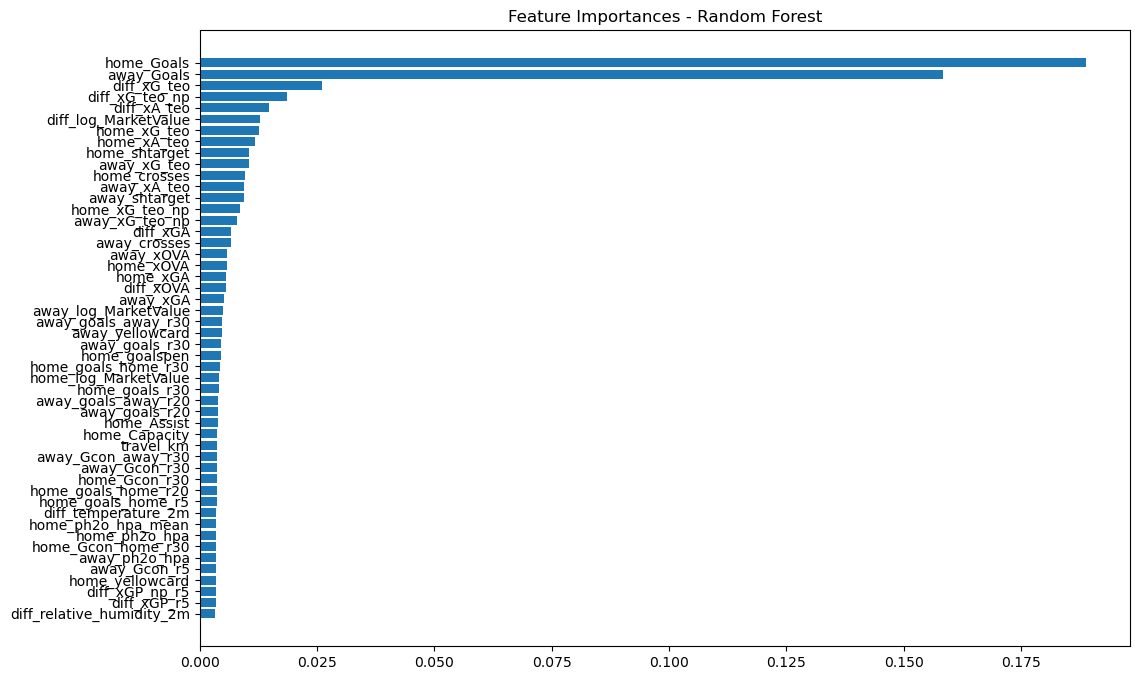
\includegraphics[width=0.9\textwidth]{primerforest.png}
	\caption{Distribuci\'on de la importancia de las caracter\'isticas en el primer clasificador Random Forest. Las dos variables dominantes son los goles del local y del visitante, lo que evidencia fuga de informaci\'on.}
	\label{fig:PrimerRandomForest}
\end{figure}

Asimismo, las variables macroecon\'omicas (PIB, inflaci\'on, Gini, gasto p\'ublico, deuda e IED) y sus transformaciones logar\'itmicas ocuparon posiciones marginales en el ranking de importancia, con valores inferiores a $0{.}004$ en todos los casos. Esto confirma su escasa se\~nal predictiva en la escala del resultado individual, en contraste con su relevancia documentada a nivel de temporada completa.

Con base en este diagn\'ostico se decidi\'o eliminar todas las variables derivadas directamente de los marcadores finales (\texttt{home\_Goals}, \texttt{away\_Goals} y sus promedios m\'oviles asociados); descartar el bloque macroecon\'omico del conjunto de caracter\'isticas activas, conserv\'andolo en el conjunto de datos maestro por reproducibilidad pero excluy\'endolo del modelo predictivo; y excluir las variables intermedias que presentaran redundancia con los \'indices compuestos de autor\'ia o que compartieran la misma fuente de fuga que los goles.

\paragraph{Segundo diagn\'ostico: filtrado y an\'alisis de importancias.} Sobre las decisiones anteriores se obtuvo un conjunto de datos filtrado que excluye las variables de fuga y conserva \'unicamente m\'etricas ex\'ogenas genuinamente disponibles antes del partido, m\'as las m\'etricas \textit{rolling} hist\'oricas. El mismo clasificador Random Forest se reentren\'o sobre este conjunto, con id\'entica partici\'on temporal.

El desempe\~no cay\'o dr\'asticamente a una \emph{accuracy} de $0{.}4879$ y un $F1$-score macro de $0{.}37$ sobre el conjunto de prueba, con las m\'etricas por clase recogidas en la parte derecha de la Tabla~\ref{tab:rf_diagnostico}.


La ca\'ida de m\'as de cuarenta puntos porcentuales en \emph{accuracy} al eliminar las variables de fuga confirma que la predicci\'on de resultados de f\'utbol es un problema de alta entrop\'ia cuando se restringe a informaci\'on disponible antes del partido. La matriz de confusi\'on (Figura~\ref{fig:SegundaMatrizConfusion}) revel\'o el patr\'on caracter\'istico ya discutido en el Marco Te\'orico: la clase empate colapsa casi por completo bajo una regla de decisi\'on dura $\arg\max$, con un \emph{recall} de apenas $0{.}03$, mientras que el modelo confunde sistem\'aticamente victorias locales y visitantes.

\begin{figure}[htbp]
	\centering
	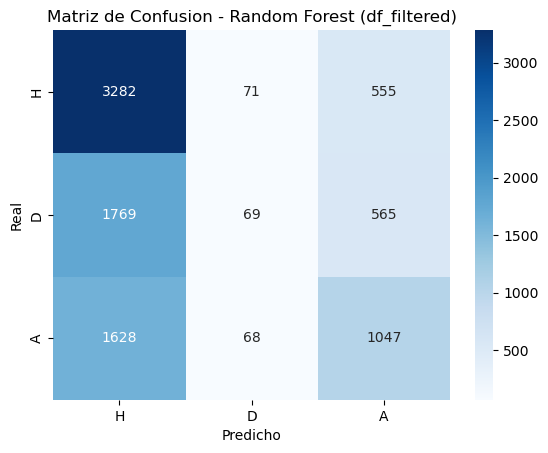
\includegraphics[width=0.9\textwidth]{matrizconfusion2.png}
	\caption{Matriz de confusi\'on del clasificador Random Forest sobre el conjunto filtrado. La clase empate colapsa bajo la regla $\arg\max$, en l\'inea con la dificultad estructural documentada en la Secci\'on~\ref{subsec:clasificacion}.}
	\label{fig:SegundaMatrizConfusion}
\end{figure}

El an\'alisis de importancias de Gini del modelo filtrado (Figura~\ref{fig:SegundoRandomForest}) permite identificar las variables con mayor peso relativo. Las seis covariables de mayor importancia fueron:
\begin{itemize}
	\item \texttt{diff\_MarketValue} ($0{.}0745$).
	\item \texttt{home\_Assist} ($0{.}0253$).
	\item \texttt{diff\_TDA} ($0{.}0224$).
	\item \texttt{diff\_xGP\_r5} ($0{.}0194$).
	\item \texttt{diff\_DDI} ($0{.}0190$).
	\item \texttt{travel\_km} ($0{.}0189$).
\end{itemize}
El resto de las variables present\'o importancias entre $0{.}010$ y $0{.}019$, sin una jerarqu\'ia pronunciada. Esta distribuci\'on, mucho m\'as plana que la del primer modelo, refleja que una vez eliminada la fuga de informaci\'on el problema se vuelve 
genuinamente dif\'icil y la se\~nal predictiva se distribuye entre m\'ultiples covariables. La variable \texttt{diff\_TDA} es un componente del \'indice de eficiencia defensiva \texttt{diff\_DDI}; su presencia individual en el ranking no implica que deba retenerse por separado, pues su informaci\'on ya est\'a capturada por el \'indice compuesto. El an\'alisis de selecci\'on multivariante de la subsecci\'on siguiente resuelve esta redundancia.

\begin{figure}[htbp]
	\centering
	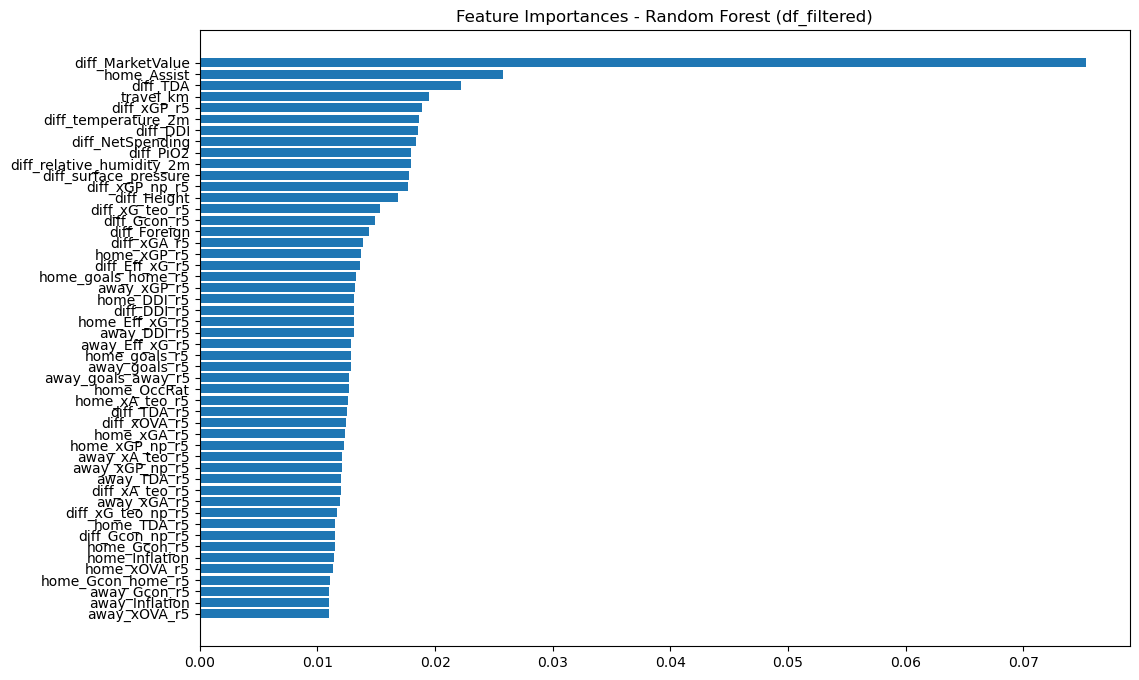
\includegraphics[width=0.9\textwidth]{segundoforest.png}
	\caption{Distribuci\'on de la importancia de las caracter\'isticas en el segundo clasificador Random Forest, tras eliminar las variables con fuga de informaci\'on.}
	\label{fig:SegundoRandomForest}
\end{figure}

En conjunto, los dos diagn\'osticos por Random Forest reducen el universo de aproximadamente 192 variables derivadas a un conjunto acotado de covariables candidatas, descartando las fuentes de fuga y las redundancias estructurales. Sobre ese conjunto acotado se aplican a continuaci\'on tres criterios de selecci\'on complementarios, con el objetivo de construir un ranking consolidado y fijar el vector de entrada del modelo de refinamiento.

\subsection{Criterios de selecci\'on multivariante}
\label{subsec:criterios_seleccion}

Sobre el subconjunto de covariables candidatas resultante del diagn\'ostico anterior se aplicaron tres criterios complementarios de selecci\'on, con el objetivo de combinar informaci\'on de distinta naturaleza estad\'istica y de depurar la redundancia residual entre variables afines. A diferencia de los clasificadores Random Forest empleados en las dos diagn\'osticos previos, cuyo universo de variables derivadas era m\'as amplio y a\'un reten\'ia variables redundantes, los tres criterios de esta subsecci\'on operan exclusivamente sobre el conjunto final de covariables candidatas. En consecuencia, las importancias relativas que se reportan a continuaci\'on no son directamente comparables con las de la Secci\'on~\ref{subsec:segunda_pasada}. Los tres criterios son: la correlaci\'on de Spearman \cite{spearman1904} de cada variable con el resultado codificado ordinalmente (victoria local $=2$, empate $=1$, victoria visitante $=0$), tomada en valor absoluto; la importancia de Gini de un clasificador Random Forest reentrenado sobre el mismo conjunto, que captura asociaciones no lineales y de orden superior; y el coeficiente promedio de una regresi\'on log\'istica con penalizaci\'on $L_1$, que induce esparsidad al anular los coeficientes de variables redundantes. Las covariables se estandarizaron previamente para el tercer criterio, ya que la penalizaci\'on $L_1$ opera sobre magnitudes.

Cada criterio se normaliz\'o al intervalo $[0,1]$ mediante escalamiento MinMax y los tres valores normalizados se sumaron para producir un \emph{score} consolidado por variable. Este score alcanza su valor m\'aximo posible de $3{.}000$ cuando una variable ocupa la primera posici\'on en los tres criterios simult\'aneamente. La Tabla~\ref{tab:ranking_variables} presenta el ranking consolidado para los conjuntos de datos Lite y Full.

\begin{table}[htbp]
	\centering
	\caption{Ranking consolidado de importancia de variables para los conjuntos de datos Lite y Full. Las columnas ``Sp.'', ``RF'' y ``L1'' corresponden a la correlaci\'on de Spearman (valor absoluto), la importancia en Random Forest y el coeficiente $L_1$ promedio (absoluto entre clases), respectivamente. El score total es la suma de los tres criterios normalizados con MinMax, con m\'aximo posible de $3{.}000$.}
	\label{tab:ranking_variables}
	\small
	\begin{tabular}{lcccc|lcccc}
		\toprule
		& \multicolumn{4}{c}{\textbf{Dataset Lite}} & & 
		\multicolumn{4}{c}{\textbf{Dataset Full}} \\
		\cmidrule(lr){2-5} \cmidrule(lr){7-10}
		\textbf{Variable} & \textbf{Sp.} & \textbf{RF} & 
		\textbf{L1} & \textbf{Total} & & \textbf{Sp.} & 
		\textbf{RF} & \textbf{L1} & \textbf{Total} \\
		\midrule
		diff\_MarketValue & 0.274 & 0.170 & 0.205 & 3.000 & & 0.276 & 0.134 & 0.194 & 3.000 \\
		diff\_xG\_teo\_r5 & ---   & ---   & ---   & ---   & & 0.158 & 0.082 & 0.077 & 1.218 \\
		home\_Assist & 0.108 & 0.114 & 0.060 & 1.018 & & 0.112 & 0.088 & 0.058 & 1.033 \\
		travel\_km & 0.034 & 0.134 & 0.022 & 0.783 & & 0.037 & 0.098 & 0.024 & 0.724 \\
		diff\_NetSpending & 0.053 & 0.117 & 0.002 & 0.570 & & 0.052 & 0.091 & 0.009 & 0.604 \\
		diff\_PiO2 & 0.006 & 0.141 & 0.015 & 0.731 & & 0.012 & 0.101 & 0.002 & 0.568 \\
		diff\_xA\_teo\_r5 & --- & --- & ---   & --- & & 0.041 & 0.081 & 0.028 & 0.519 \\
		home\_OccRat & 0.047 & 0.109 & 0.003 & 0.459 & & 0.047 & 0.083 & 0.005 & 0.447 \\
		diff\_temperature\_2m & 0.013 & 0.131 & 0.002 & 0.580 & & 0.001 & 0.095 & 0.002 & 0.436 \\
		diff\_DDI\_r5 & --- & --- & --- & ---  & & 0.017 & 0.081 & 0.010 & 0.327 \\
		diff\_Foreign & 0.055 & 0.083 & 0.002 & 0.181 & & 0.043 & 0.065 & 0.008 & 0.185 \\
		\bottomrule
	\end{tabular}
\end{table}

\subsection{An\'alisis de ablaci\'on y conjunto final de covariables}
\label{subsec:conjunto_final}

Para cuantificar el aporte marginal de las covariables candidatas, se realiz\'o un an\'alisis de ablaci\'on \emph{leave-one-out} mediante validaci\'on cruzada con 10 particiones aleatorias (\emph{shuffle}), utilizando el mismo clasificador Random Forest y comparando los resultados con pruebas $t$ pareadas. Es importante destacar que este an\'alisis tiene prop\'osito de diagn\'ostico, no de reporte del rendimiento final del sistema; las m\'etricas aqu\'i obtenidas no son directamente comparables con las del \textit{pipeline} principal, que utiliza una partici\'on cronol\'ogica estricta.

\paragraph{Resultados sobre los conjuntos de datos Lite y Full.} Los 
resultados de la ablaci\'on se resumen en la 
Tabla~\ref{tab:ablacion}. Ninguna de las diferencias entre configuraciones alcanza significancia al $5\%$, ni en \emph{accuracy} ni en $F1$-macro, en ninguno de los dos conjuntos de datos.

\begin{table}[htbp]
	\centering
	\caption{An\'alisis de ablaci\'on por validaci\'on cruzada con 
		10 particiones. Media $\pm$ desviaci\'on est\'andar y 
		$p$-valor del test $t$ pareado contra la configuraci\'on 
		completa.}
	\label{tab:ablacion}
	\small
	\begin{tabular}{llcccc}
		\toprule
		& & \multicolumn{2}{c}{\textbf{Dataset Lite}} & 
		\multicolumn{2}{c}{\textbf{Dataset Full}} \\
		\cmidrule(lr){3-4} \cmidrule(lr){5-6}
		\textbf{M\'etrica} & \textbf{Configuraci\'on} & 
		Valor & $p$ & Valor & $p$ \\
		\midrule
		\multirow{3}{*}{Accuracy}
		& Todas las variables          & $0.4550 \pm 0.0066$ & ---     & $0.4638 \pm 0.0103$ & --- \\
		& Sin \texttt{home\_OccRat}    & $0.4562 \pm 0.0060$ & 0.4564  & $0.4626 \pm 0.0075$ & 0.6805 \\
		& Sin \texttt{travel\_km}      & $0.4571 \pm 0.0053$ & 0.3780  & $0.4636 \pm 0.0087$ & 0.9505 \\
		\midrule
		\multirow{3}{*}{$F1$-macro}
		& Todas las variables          & $0.3955 \pm 0.0084$ & ---     & $0.3921 \pm 0.0078$ & --- \\
		& Sin \texttt{home\_OccRat}    & $0.3965 \pm 0.0055$ & 0.6177  & $0.3904 \pm 0.0085$ & 0.5364 \\
		& Sin \texttt{travel\_km}      & $0.4005 \pm 0.0049$ & 0.0817  & $0.3936 \pm 0.0077$ & 0.5784 \\
		\bottomrule
	\end{tabular}
\end{table}

Los resultados anteriores muestran que ninguna de las covariables candidatas aporta una mejora estad\'isticamente significativa al modelo por s\'i sola: todas las diferencias entre configuraciones son compatibles con la hip\'otesis nula de aporte nulo. La decisi\'on de retenci\'on se apoy\'o entonces en dos criterios complementarios: la existencia de redundancia estructural entre variables afines, y la posici\'on relativa de cada covariable en el ranking consolidado de la Tabla~\ref{tab:ranking_variables}. Los dos casos que requieren discusi\'on expl\'icita son \texttt{home\_OccRat} y \texttt{travel\_km}.

\paragraph{Decisi\'on sobre \texttt{home\_OccRat}.} La variable 
\texttt{home\_OccRat} es una transformaci\'on determinista de \texttt{home\_Assist} (Ecuaci\'on~\ref{eq:OccRat}), lo que genera una redundancia estructural entre ambas. El ranking consolidado muestra que \texttt{home\_Assist} supera consistentemente a \texttt{home\_OccRat} en los tres criterios considerados: $1{.}018$ vs $0{.}459$ en el Dataset Lite y $1{.}033$ vs $0{.}447$ en el Dataset Full. El an\'alisis de ablaci\'on confirma que la exclusi\'on de \texttt{home\_OccRat} no degrada el rendimiento ($p > 0.45$ en ambos conjuntos de datos). En consecuencia, se descarta \texttt{home\_OccRat} y se retiene \texttt{home\_Assist} como representante del bloque de estadio y afici\'on. La Tabla~\ref{tab:correlacion_spearman} reporta la matriz de correlaci\'on de rangos entre las covariables del bloque ex\'ogeno, que respalda esta decisi\'on desde el \'angulo de los coeficientes de Spearman.

\begin{table}[htbp]
	\centering
	\caption{Coeficientes de correlaci\'on de Spearman entre las covariables del bloque ex\'ogeno, para los pares con $|\rho| > 0{.}10$. La matriz se calcul\'o sobre las covariables disponibles al momento del an\'alisis de selecci\'on; no incluye \texttt{diff\_NetSpending} ni \texttt{travel\_km}, incorporadas al conjunto final con posterioridad.}
	\label{tab:correlacion_spearman}
	\begin{tabular}{lcc}
		\toprule
		\textbf{Par de variables} & \textbf{Lite} & \textbf{Full} \\
		\midrule
		\texttt{home\_Assist}--\texttt{home\_OccRat} & $0{.}784$ & $0{.}753$ \\
		\texttt{diff\_MarketValue}--\texttt{diff\_xG\_teo\_r5} & --- & $0{.}310$ \\
		\texttt{diff\_MarketValue}--\texttt{diff\_Foreign} & $0{.}225$ & $0{.}220$ \\
		\texttt{diff\_MarketValue}--\texttt{home\_Assist} & $0{.}216$ & $0{.}224$ \\
		\texttt{diff\_temperature\_2m}--\texttt{diff\_PiO2} & $0{.}194$ & $0{.}101$ \\
		\texttt{diff\_xG\_teo\_r5}--\texttt{diff\_xA\_teo\_r5} & --- & $0{.}119$ \\
		\bottomrule
	\end{tabular}
\end{table}

El \'unico par de covariables que supera el umbral de $0{.}5$ es \texttt{home\_Assist}--\texttt{home\_OccRat}, con $0{.}784$ en Lite y $0{.}753$ en Full, lo que confirma cuantitativamente la redundancia estructural entre ambas. Los pares restantes se mantienen por debajo de $0{.}35$, y la mayor\'ia por debajo de $0{.}25$. Los tres pares que involucran a \texttt{diff\_MarketValue} con \texttt{diff\_xG\_teo\_r5}, \texttt{diff\_Foreign} y \texttt{home\_Assist} presentan coeficientes en torno a $0{.}22$ y son consistentes con la interpretaci\'on de que el valor de mercado funciona como un indicador agregado de la calidad del club, que se refleja simult\'aneamente en la generaci\'on de ocasiones, la composici\'on de la plantilla y el respaldo de la afici\'on. La baja correlaci\'on entre \texttt{diff\_temperature\_2m} y \texttt{diff\_PiO2} confirma que, aunque ambas variables pertenecen al bloque ambiental, capturan efectos f\'isicos distintos. En conjunto, la matriz respalda la decisi\'on de descartar \texttt{home\_OccRat} y confirma que las covariables restantes son suficientemente independientes entre s\'i para alimentar el refinamiento no lineal sin inducir multicolinealidad.

\paragraph{Decisi\'on sobre \texttt{travel\_km}.} La variable \texttt{travel\_km} presenta un $p$-valor de $0{.}3780$ en el Dataset Lite y $0{.}9505$ en el Full, lo que indica que su eliminaci\'on no afecta significativamente la \emph{accuracy} en ning\'un caso. Su relevancia en el ranking consolidado es alta (posici\'on 3 en Lite con score $0{.}783$, posici\'on 4 en Full con $0{.}724$). En el Dataset Lite, su eliminaci\'on mejora marginalmente el $F1$-macro ($0{.}3955 \to 0{.}4005$, $p = 0{.}0817$) y la \emph{accuracy} ($0{.}4550 \to 0{.}4571$), sin alcanzar significancia al $5\%$; en el Dataset Full el efecto es nulo. Dado que la literatura base sobre ventaja de local\'ia se\~nala el desplazamiento geogr\'afico como un factor estructural \cite{Glicko2Mod}, y que su efecto sobre el desempe\~no es despreciable en ambos conjuntos de datos, se decide mantener \texttt{travel\_km} en el conjunto final.

\paragraph{Conjunto final de covariables ex\'ogenas.} El conjunto activo que alimenta el perceptr\'on multicapa queda conformado por siete variables en el Dataset Lite y el Dataset Lite Recortado, y diez en el Dataset Full:

\begin{itemize}
	\item \textbf{Bloque econ\'omico:} \texttt{diff\_MarketValue}, \texttt{diff\_NetSpending}.
	\item \textbf{Bloque de composici\'on de plantilla:} \texttt{diff\_Foreign}.
	\item \textbf{Bloque ambiental y geogr\'afico:} \texttt{diff\_temperature\_2m}, \texttt{diff\_PiO2}, \texttt{travel\_km}.
	\item \textbf{Bloque de estadio y afici\'on:} \texttt{home\_Assist}.
	\item \textbf{Bloque deportivo} (solo en el Dataset Full): \texttt{diff\_xG\_teo\_r5}, \texttt{diff\_xA\_teo\_r5}, \texttt{diff\_DDI\_r5}.
\end{itemize}

Este vector, junto con las tres probabilidades base $(P_H, P_D, P_A)$ generadas por el sistema de rating y el modelo de conteo, constituye el input $\mathbf{z}_{ij} \in \mathbb{R}^{d}$ del MLP, donde $d=10$ en el Dataset Lite y Lite Recortado, y $d=13$ en el Dataset Full. La reducci\'on dimensional busc\'o mitigar el sobreajuste en la fase de refinamiento no lineal, aunque el dr\'astico descenso de \emph{accuracy} entre el primer y segundo diagn\'ostico del Random Forest sugiere que el cuello de botella del sistema no reside en la dimensionalidad, sino en la alta varianza inherente al fen\'omeno deportivo. El an\'alisis detallado del desempe\~no predictivo del \textit{pipeline} completo se reserva para el Cap\'itulo~\ref{ch:resultados}.

% ============================================================
% SECCION 3.4 -- Arquitectura y calibracion del sistema predictivo
% ============================================================

\section{Arquitectura y calibraci\'on del sistema predictivo}
\label{sec:arquitectura}

El sistema predictivo se organiza como un \textit{pipeline} de tres bloques funcionales encadenados: un bloque de conteo que estima las tasas de goles y deriva una probabilidad de empate; un bloque de rating din\'amico que actualiza secuencialmente la fuerza latente de los equipos y genera un vector de probabilidades base; y un bloque de refinamiento no param\'etrico que corrige dichas probabilidades mediante un perceptr\'on multicapa alimentado con covariables ex\'ogenas. Esta secci\'on documenta las decisiones de dise\~no de cada bloque y el procedimiento de calibraci\'on utilizado, respetando estrictamente el orden de dependencias del sistema: el bloque de conteo se entrena primero, sus predicciones alimentan la calibraci\'on del rating, y las probabilidades base de este \'ultimo alimentan el entrenamiento del refinador neuronal. Los valores num\'ericos obtenidos en cada etapa de calibraci\'on y entrenamiento se reportan en el Cap\'itulo~\ref{ch:resultados}.

La variable a predecir en todos los bloques es el resultado del partido al finalizar el tiempo reglamentario, codificada en tres clases mutuamente excluyentes: victoria del equipo local ($H$), empate ($D$) o victoria del equipo visitante ($A$). La codificaci\'on operativa difiere entre bloques seg\'un la naturaleza de cada uno. En el bloque de rating se representa mediante el escalar $s_j \in \{1, 0{.}5, 0\}$ seg\'un el resultado observado, notaci\'on can\'onica de los sistemas Elo y Glicko. Para el bloque de refinamiento (MLP), la codificaci\'on se transforma a un vector indicador \emph{one-hot} $\mathbf{y}_i \in \{0,1\}^3$, donde la componente correspondiente a la clase observada toma valor $1$ y las restantes $0$.

\subsection{Bloque de conteo: estimaci\'on de tasas y probabilidad de empate}
\label{subsec:conteo}

El primer bloque modela el n\'umero de goles anotados por cada equipo como un proceso de conteo independiente, siguiendo el marco te\'orico de la Secci\'on~\ref{sec:modelo_probabilistico}. Se entrenan dos regresores LightGBM con funci\'on objetivo Poisson \cite{ke2017lightgbm}, uno para los goles del equipo local ($\lambda_H$) y otro para los del visitante ($\lambda_A$).

\paragraph{Partici\'on temporal.} La partici\'on respeta el orden cronol\'ogico: el $70\%$ inicial de los partidos (ordenados por \texttt{match\_date\_from\_id}) constituye el conjunto de entrenamiento; el $30\%$ restante, el de prueba. Dentro del entrenamiento se reserva un $10\%$ final para \emph{early stopping}. Este dise\~no evita la fuga de informaci\'on temporal y garantiza que el modelo solo utiliza partidos anteriores a los de prueba.

\paragraph{Variables de entrada.} Dado que el objetivo de este bloque es capturar la din\'amica de forma reciente sin introducir fuga del resultado final, \'unicamente se utilizan las variables de promedios m\'oviles de goles anotados y recibidos en ventanas de $5$, $10$, $20$ y $30$ partidos, diferenciadas por condici\'on de local\'ia. Espec\'ificamente, las entradas son $32$ columnas que cruzan cuatro dimensiones:
\begin{enumerate}
	\item El prefijo indica si la estad\'istica corresponde al equipo 	local (\texttt{home}) o al visitante (\texttt{away}).
	\item La ra\'iz distingue entre goles marcados (\texttt{goals}) y goles recibidos (\texttt{Gcon}).
	\item Para cada prefijo se generan dos versiones: la global, sin sufijo adicional, y la condicionada a partidos jugados en la condici\'on del prefijo.
	\item El sufijo final determina el tama\~no de la ventana, que puede ser $5$, $10$, $20$ o $30$ partidos.
\end{enumerate}
El producto de estas dimensiones, $2 \times 2 \times 2 \times 4 = 32$, da como resultado las $32$ columnas del grupo.

\paragraph{Hiperpar\'ametros.} Los modelos se configuran con \texttt{n\_estimators}$=200$, \texttt{learning\_rate}$=0{.}05$, \texttt{max\_depth}$=5$ y criterio de parada temprana de $10$ iteraciones sin mejora en el MAE de validaci\'on. La m\'etrica de evaluaci\'on interna es el error absoluto medio, coherente con la escala de conteo de los goles.

\paragraph{Derivaci\'on de la probabilidad de empate.} A partir de las tasas predichas $\hat{\lambda}_H$ y $\hat{\lambda}_A$, se calcula la probabilidad de empate mediante la distribuci\'on de Skellam evaluada en $k=0$ (Ecuaci\'on~\ref{eq:prob_D_bessel} del Cap\'itulo~\ref{ch:marco}):
\begin{equation}
	\hat{P}_D^{(S)} = e^{-(\hat{\lambda}_H + \hat{\lambda}_A)} \, 
	I_0\!\left(2\sqrt{\hat{\lambda}_H \hat{\lambda}_A}\right).
\end{equation}
Este valor, denominado \texttt{draw\_prob} en el \textit{pipeline}, se anexa al conjunto de datos y alimenta el bloque de rating como estimaci\'on externa de la frecuencia de empates.

\subsection{Bloque de rating: Glicko-2 modificado}
\label{subsec:rating}

El n\'ucleo inferencial del sistema es una implementaci\'on propia basada en el algoritmo Glicko-2 modificado de Shelopugin y Sirotkin \cite{Glicko2Mod}, contenida en el m\'odulo \texttt{G2Av1513.py}. A diferencia del motor can\'onico de referencia (\texttt{glicko2.py}), esta implementaci\'on incorpora varias mejoras de mecanismos num\'ericos y coherencia probabil\'istica que se detallan a continuaci\'on.

\subsubsection{Diferencias frente al motor de referencia}
\label{subsubsec:mejoras_g2av1513}

El motor \texttt{G2Av1513.py} se construy\'o sobre el c\'odigo can\'onico de Shelopugin y Sirotkin (\texttt{glicko2.py}), del cual hereda la estructura de actualizaci\'on bayesiana del Glicko-2. Sobre esa base se introdujeron tres clases de modificaciones, que se distinguen por su naturaleza: correcciones algebraicas que alteran el comportamiento probabil\'istico del modelo, decisiones de calibraci\'on emp\'irica respaldadas por barridos de hiperpar\'ametros, y mecanismos de estabilidad num\'erica que preservan el comportamiento del motor en condiciones extremas sin alterar sus predicciones en r\'egimen normal. Se documentan tambi\'en dos extensiones funcionales que quedaron implementadas pero no activadas en el \textit{pipeline} principal.

\paragraph{Correcci\'on del denominador trinomial.} El motor de referencia computa las tres probabilidades mediante dos denominadores asim\'etricos respecto al t\'ermino de empate. La probabilidad de victoria local surge del denominador $1 + (1 + e^{d+P_D^{(S)}})/e^{\delta}$ y la de victoria visitante de $1 + (1 + e^{d+P_D^{(S)}})e^{\delta}$, donde $\delta = g(\phi_j)(\mu - \mu_j)$ es la diferencia de ratings efectiva y $P_D^{(S)}$ la probabilidad de empate derivada de la distribuci\'on de Skellam. La probabilidad de empate se obtiene por complemento, $P_D = 1 - P_H - P_A$. Esta construcci\'on asigna al par\'ametro $d$ un efecto que depende de $\delta$ en lugar de operar como t\'ermino sim\'etrico del empate: a medida que la diferencia de ratings crece, el denominador de la victoria visitante crece con $\delta$ y el de la victoria local decrece, de modo que el empate queda estructuralmente penalizado en partidos desequilibrados. El motor propio unifica el denominador como
\begin{equation}
	1 + \exp(\delta) + \exp(d + P_{D,\text{logit}}^{(S)}),
\end{equation}
garantizando que las tres probabilidades provengan de una partici\'on sim\'etrica del simplex y que $d$ act\'ue como un t\'ermino aditivo puro sobre la masa del empate.

\paragraph{Reparametrizaci\'on logit del par\'ametro de empate.} El motor can\'onico alimenta la probabilidad de empate cruda $P_D^{(S)} \in (0,1)$ directamente al exponente $\exp(d+P_D^{(S)})$. Como $P_D^{(S)}$ var\'ia aproximadamente en $[0.2, 0.3]$ en el rango operativo del f\'utbol profesional, el t\'ermino $\exp(d+P_D^{(S)})$ es pr\'acticamente constante y el par\'ametro de empate resulta funcionalmente inerte frente a la se\~nal del modelo de conteo. La implementaci\'on propia aplica la transformaci\'on logit
\begin{equation}
	P_{D,\text{logit}}^{(S)} = \ln\!\left(\frac{P_{D}^{(S)}}{1-P_{D}^{(S)}}\right),
\end{equation}
que mapea $(0,1)$ sobre la recta real y preserva la variabilidad de la se\~nal de Skellam dentro del exponente. Esta correcci\'on es funcional, no un simple cambio de escala, pues altera la forma en que el modelo responde a variaciones en la probabilidad de empate del bloque de conteo.

\paragraph{Calibraci\'on emp\'irica de la constante de atenuaci\'on y la volatilidad.} Dos hiperpar\'ametros heredados del motor can\'onico fueron reajustados mediante un barrido emp\'irico sobre el panel multiliga. La constante de atenuaci\'on $g$ del factor $g(\phi_j)$ pas\'o de $1{.}5/\pi^2$ a $3{.}0/\pi^2$, lo que suaviza la superficie de p\'erdida del optimizador y reduce la sensibilidad del rating a la diferencia de desviaciones entre equipos. La constante de difusi\'on temporal $\tau$ pas\'o de $1{.}0$ a $0{.}8$, valor que produce una trayectoria de volatilidad m\'as estable sobre el panel utilizado. Ambos ajustes se derivaron de un barrido de configuraciones previo a la arquitectura en cascada final y se fijaron por su desempe\~no en la log-loss de validaci\'on del bloque de rating en aislamiento.

\paragraph{Mecanismos de estabilidad num\'erica.} La calibraci\'on por L-BFGS-B sobre un panel multiliga expone al motor a reg\'imenes num\'ericos extremos que el c\'odigo can\'onico no contempla. Se a\~nadieron acotamientos sobre la diferencia de ratings efectiva, sobre la puntuaci\'on esperada antes del c\'alculo de la varianza $v$, sobre las probabilidades finales del simplex, y una protecci\'on contra divisi\'on por cero en la funci\'on de varianza. Estos mecanismos no alteran el comportamiento del motor en r\'egimen normal; su funci\'on es evitar indeterminaciones num\'ericas cuando el optimizador explora regiones alejadas del \'optimo durante la calibraci\'on.

\paragraph{Extensiones funcionales no activadas.} El motor propio incorpora dos extensiones que no se utilizan en el \textit{pipeline} del presente trabajo pero quedan disponibles para desarrollos futuros. La primera es un sistema de ventaja parametrizada: mientras el motor can\'onico recibe un escalar fijo \texttt{advantage}, el motor propio acepta un vector de covariables y calcula la ventaja efectiva como combinaci\'on lineal $h_{\text{eff}} = \beta_0 + \sum_k \beta_k f_k$. En la versi\'on calibrada esta flexibilidad se emplea \'unicamente para inyectar la ventaja de local\'ia por liga $h_\ell$ como \'unico para\'ametro activo, dejando la infraestructura disponible para extensiones. La segunda corresponde a una atenuaci\'on multiplicativa de la ventaja de local\'ia, definida originalmente para ser utilizada durante el per\'iodo marzo 2020--junio 2021, durante la pandemia global de la COVID-19, esta funci\'on se encuentra descrita en el trabajo base pero no implementada en su c\'odigo. En esta implementaci\'on la extensi\'on est\'a codificada y se activa con un indicador binario; en todas las ejecuciones del presente trabajo dicho indicador toma valor $0$.

La Tabla~\ref{tab:constantes_divergentes} consolida los hiperpar\'ametros donde la implementaci\'on propia se aparta del valor can\'onico de Glicko-2 o del motor de referencia de Shelopugin y Sirotkin. Los tres valores se fijaron emp\'iricamente mediante un barrido de configuraciones previo a la arquitectura en cascada final; no provienen de una regla derivada de la literatura, sino de su desempe\~no en la log-loss de validaci\'on del bloque de rating en aislamiento.

\begin{table}[htbp]
	\centering
	\caption{Hiperpar\'ametros donde la implementaci\'on se aparta del valor can\'onico.}
	\label{tab:constantes_divergentes}
	\small
	\begin{tabular}{p{2.8cm} p{2.6cm} p{2.6cm} p{6.4cm}}
		\toprule
		\textbf{Par\'ametro} & \textbf{Valor can\'onico} & \textbf{Valor implementado} & \textbf{Justificaci\'on} \\
		\midrule
		$RD_0$ & $350$ & $80$ & La calibraci\'on preliminar mostr\'o una convergencia m\'as estable del optimizador sobre el panel multiliga. \\
		$\tau$ & $1{.}0$ & $0{.}8$ & El barrido emp\'irico produjo una trayectoria de volatilidad m\'as estable sobre el panel utilizado. \\
		$g_{\text{constant}}$ & $1{.}5/\pi^2$ & $3{.}0/\pi^2$ & Suaviza la superficie de p\'erdida del optimizador y reduce la sensibilidad del rating a la diferencia de desviaciones entre equipos. \\
		\bottomrule
	\end{tabular}
\end{table}

\begin{obs}[Sobre la funci\'on de actualizaci\'on de volatilidad]
	Tanto el motor can\'onico de Shelopugin y Sirotkin como la implementaci\'on propia omiten el factor $\tau^2$ en el denominador del segundo t\'ermino de la funci\'on $f(x)$ del Paso~5 del algoritmo Glicko-2. Esta simplificaci\'on, heredada del c\'odigo fuente de referencia, no impide la convergencia del m\'etodo de Illinois empleado para la estimaci\'on de $\sigma'$, aunque desv\'ia ligeramente la trayectoria de optimizaci\'on respecto a la formulaci\'on can\'onica de Glickman \cite{Glickman2022}. Dado que ambos motores comparten esta misma estructura, no se documenta como diferencia del presente trabajo.
\end{obs}

\subsubsection{Calibraci\'on por m\'axima verosimilitud}
\label{subsubsec:calibracion_glicko}

El bloque de rating se calibra sobre cada conjunto de datos por separado mediante la minimizaci\'on de la log-verosimilitud negativa del resultado observado. Formalmente, sea $\mathcal{D}_{\text{train}}$ el conjunto de partidos ordenados cronol\'ogicamente. Para cada partido $i$, el modelo genera el vector $(P_{H,i}, P_{D,i}, P_{A,i})$ seg\'un las Ecuaciones~\eqref{eq:prob_victoria_local}--\eqref{eq:prob_victoria_visitante} del Cap\'itulo~\ref{ch:marco}, y actualiza secuencialmente los ratings de ambos equipos. La funci\'on objetivo es
\begin{equation}
	\mathcal{L}_{\text{G2A}}(d, \{\mu_{\text{init},\ell}\}, \{h_\ell\}) 
	= -\frac{1}{|\mathcal{D}_{\text{train}}|}
	\sum_{i \in \mathcal{D}_{\text{train}}} \log P_{o_i,i},
\end{equation}
donde $o_i \in \{H,D,A\}$ es el resultado observado y $P_{o_i,i}$ la probabilidad asignada a dicha clase.

\paragraph{Espacio de par\'ametros y cotas.} El optimizador L-BFGS-B \cite{byrd1995limited} ajusta simult\'aneamente los hiperpar\'ametros estructurales del bloque, restringidos a intervalos derivados de su interpretaci\'on probabil\'istica:
\begin{itemize}
	\item El t\'ermino de calibraci\'on del empate $d \in [-5{.}0,\, 5{.}0]$.
	\item El rating inicial medio por liga 	$\mu_{\text{init},\ell} \in [1200,\, 1800]$, expresado como desviaci\'on respecto a $1500$ en el espacio de optimizaci\'on.
	\item La ventaja de local\'ia por liga $h_\ell \in [0,\, 200]$, escalada internamente por un factor $10$ en el optimizador.
\end{itemize}
Los valores semilla son $d_0 = 0{.}5$, desviaciones nulas para $\mu_{\text{init},\ell}$ y valor escalado $5{.}0$ para $h_\ell$. El n\'umero m\'aximo de iteraciones del optimizador es $400$ y el criterio de convergencia es \texttt{ftol}$=10^{-5}$. La cota del t\'ermino de empate $d$ acota la correcci\'on sobre la probabilidad derivada de Skellam dentro de un rango de sensibilidad razonable; las cotas de $\mu_{\text{init},\ell}$ restringen el rating inicial a un entorno de 300 puntos alrededor del valor can\'onico 1500; y las cotas de $h_\ell$ corresponden a un efecto m\'aximo de 200 puntos de rating, equivalente a una ventaja de local\'ia fuerte pero no arbitraria.

\paragraph{Estado e inicializaci\'on.} Cada equipo se caracteriza por el estado $(R, RD, \sigma)$. Los valores iniciales por defecto son $R_0 = 1500$, $RD_0 = 80$ y $\sigma_0 = 0{.}06$. La constante de difusi\'on temporal se fija en $\tau = 0{.}8$, valor est\'andar para conjuntos de resultados de alta volatilidad \cite{Glickman2022}. Aunque el valor can\'onico de Glickman es $RD_0=350$, en esta implementaci\'on se fija $RD_0=80$ tras una calibraci\'on preliminar que mostr\'o una convergencia m\'as estable para el panel de ligas utilizado.

Los valores calibrados de $d$, $\mu_{\text{init},\ell}$ y $h_\ell$ por liga, as\'i como las estad\'isticas de convergencia del optimizador y el rango final de ratings, se reportan en la Secci\'on~\ref{sec:res_rating} del Cap\'itulo~\ref{ch:resultados}.

\subsection{Bloque de refinamiento: perceptr\'on multicapa}
\label{subsec:mlp}

El tercer bloque corrige las probabilidades base del Glicko-2 mediante un perceptr\'on multicapa \emph{feedforward} implementado en \texttt{Keras/TensorFlow}. La elecci\'on responde al car\'acter no lineal ni aditivo de las interacciones entre covariables y resultado: los tres criterios de selecci\'on de la Secci\'on~\ref{sec:seleccion_covariables} identificaron variables con se\~nal marginal, cuya contribuci\'on conjunta solo puede capturarse mediante una funci\'on de aproximaci\'on flexible. El Teorema de Aproximaci\'on Universal (Secci\'on~\ref{sec:mlp} del Cap\'itulo~\ref{ch:marco}) garantiza que una red con una capa oculta puede aproximar cualquier funci\'on continua sobre un compacto, propiedad que sostiene el uso del MLP como refinador no param\'etrico.

\paragraph{Vector de entrada.} La entrada del MLP combina las probabilidades base del rating con las covariables ex\'ogenas seleccionadas en las Secci\'on~\ref{sec:seleccion_covariables}. Para cada partido $i$, el vector $\mathbf{z}_{ij} \in \mathbb{R}^{d}$ se construye concatenando:
\begin{itemize}
	\item Las tres probabilidades base del Glicko-2: $(P_{H,i}, P_{D,i}, P_{A,i})$.
	\item Las covariables ex\'ogenas estandarizadas seleccionadas en la Secci\'on~\ref{sec:seleccion_covariables}: siete variables en los conjuntos de datos Lite y Lite Recortado (\texttt{diff\_MarketValue}, \texttt{diff\_NetSpending}, \texttt{diff\_Foreign}, \texttt{diff\_temperature\_2m}, \texttt{diff\_PiO2}, \texttt{travel\_km}, \texttt{home\_Assist}); y esas mismas siete m\'as las tres m\'etricas deportivas \textit{rolling} (\texttt{diff\_xG\_teo\_r5}, \texttt{diff\_xA\_teo\_r5}, \texttt{diff\_DDI\_r5}) en el Dataset Full.
\end{itemize}
En consecuencia, $d = 10$ para el Dataset Lite y el Dataset Lite Recortado, y $d = 13$ para el Dataset Full. La estandarizaci\'on de media cero y varianza unitaria se ajusta exclusivamente sobre el conjunto de entrenamiento mediante \texttt{StandardScaler} de \texttt{scikit-learn} y se aplica al conjunto de prueba.

\paragraph{Arquitectura e hiperpar\'ametros.} La red se estructura con dos capas ocultas densas de 64 neuronas cada una, precediendo una capa de salida con activaci\'on \emph{softmax} que garantiza un vector de probabilidades sobre las tres clases. La elecci\'on de ReLU en las capas ocultas y softmax en la salida sigue las recomendaciones est\'andar para clasificaci\'on multiclase \cite{solorzano2025rn}.

La profundidad de dos capas ocultas se fija por parsimonia: suficiente para capturar interacciones de segundo orden entre covariables, sin incurrir en la complejidad de una red profunda que el tama\~no del panel no justifica. La topolog\'ia resultante es:
\begin{itemize}
	\item Capa de entrada: $d$ neuronas, sin activaci\'on.
	\item Primera capa oculta: 64 neuronas, activaci\'on ReLU, \emph{dropout} con tasa $0{.}3$.
	\item Segunda capa oculta: 64 neuronas, activaci\'on ReLU, \emph{dropout} con tasa $0{.}3$.
	\item Capa de salida: 3 neuronas con activaci\'on \emph{softmax}.
\end{itemize}

\paragraph{Funci\'on de p\'erdida y optimizador.} La funci\'on de p\'erdida es la entrop\'ia cruzada categ\'orica (\texttt{categorical\_crossentropy}), equivalente a la log-verosimilitud negativa del modelo multinomial (Proposici\'on~\ref{prop:equivalencia} del Cap\'itulo~\ref{ch:marco}). El optimizador es Adam con tasa de aprendizaje inicial $\eta_0 = 10^{-3}$ y par\'ametros por defecto $\beta_1 = 0{.}9$, $\beta_2 = 0{.}999$. Se utiliza un planificador de tasa adaptativo (\texttt{ReduceLROnPlateau}) que reduce la tasa por un factor $0{.}5$ si la p\'erdida de validaci\'on no decrece durante $3$ \'epocas consecutivas. El entrenamiento se ejecuta durante $50$ \'epocas con lotes de tama\~no $64$, reservando el $10\%$ del entrenamiento para validaci\'on interna.

\paragraph{Protocolo de ejecuciones pareadas.} Dado el car\'acter estoc\'astico de la inicializaci\'on de pesos de la red y del \emph{dropout}, se ejecutan $10$ ejecuciones pareadas con semillas consecutivas (\texttt{Seed}$=42$ a \texttt{Seed}$=51$). En cada ejecuci\'on se reentrena el Glicko-2 desde cero manteniendo los hiperpar\'ametros $d$ y $h_\ell$ previamente optimizados, y se ajusta el MLP sobre las probabilidades base resultantes. Este dise\~no experimental permite estimar la varianza del desempe\~no atribuible a la aleatoriedad del optimizador neuronal y aplicar inferencia estad\'istica mediante el test $t$ pareado para comparar el modelo base (MLP sobre probabilidades Glicko-2 sin covariables) contra el modelo completo (MLP sobre probabilidades m\'as covariables ex\'ogenas). Los resultados del protocolo se reportan en la Secci\'on~\ref{sec:res_mlp} del Cap\'itulo~\ref{ch:resultados}.

\subsection{Flujo de inferencia en cascada}
\label{subsec:cascada}

El comportamiento del sistema sobre un partido nuevo sigue el orden de dependencias de sus tres bloques, sin retorno de informaci\'on desde etapas posteriores hacia anteriores. El LightGBM Poisson recibe los promedios m\'oviles de goles de ambos equipos y predice las tasas esperadas $(\hat{\lambda}_H, \hat{\lambda}_A)$, de las cuales se deriva la probabilidad de empate $\hat{P}_D^{(S)}$ mediante la distribuci\'on de Skellam. El Glicko-2 modificado consulta los estados vigentes de ambos equipos, incorpora $\hat{P}_D^{(S)}$ como par\'ametro de empate y la ventaja de local\'ia $h_\ell$ calibrada para la competici\'on, y emite el vector de probabilidades base $(P_H, P_D, P_A)$. Finalmente, el perceptr\'on multicapa recibe la concatenaci\'on de ese vector con las covariables ex\'ogenas estandarizadas del partido, y produce el vector refinado $(\tilde{P}_H, \tilde{P}_D, \tilde{P}_A)$ sobre el que se aplica la decisi\'on final.

El dise\~no garantiza que cada bloque opera sobre informaci\'on genuinamente disponible antes del partido: los promedios m\'oviles de goles son hist\'oricos, los ratings se actualizan secuencialmente sin consultar el futuro, y las covariables ex\'ogenas corresponden a datos de mercado, estadio y clima previos al encuentro. Sobre esta base, el Cap\'itulo~\ref{ch:resultados} reporta el desempe\~no emp\'irico del sistema completo sobre los tres conjuntos de datos, as\'i como las comparaciones internas entre bloques y las pruebas de inferencia estad\'istica que sustentan las conclusiones del trabajo.

% ============================================================
% SECCION 3.5 -- Metricas de evaluacion
% ============================================================

\section{M\'etricas de evaluaci\'on}
\label{sec:metricas_eval}

El dise\~no del sistema predictivo exige un esquema de evaluaci\'on que distinga entre calibraci\'on probabil\'istica y capacidad de clasificaci\'on dura. Como se establece en la Secci\'on~\ref{sec:metricas} del Cap\'itulo~\ref{ch:marco}, la log-loss categ\'orica constituye la m\'etrica central de optimizaci\'on porque es una regla de puntuaci\'on estrictamente propia: incentiva al modelo a reportar la probabilidad verdadera de cada resultado sin forzar una apuesta binaria. No obstante, para complementar el an\'alisis y mantener comparabilidad con la literatura base \cite{Glicko2Mod}, se reportan tambi\'en m\'etricas de clasificaci\'on y un protocolo de inferencia estad\'istica sobre ejecuciones pareadas. Esta secci\'on documenta las definiciones operativas de cada m\'etrica y el protocolo experimental que gobierna su interpretaci\'on; los valores obtenidos se reportan en el Cap\'itulo~\ref{ch:resultados}.

\subsection{M\'etricas de evaluaci\'on del sistema}
\label{subsec:metricas_prob}
\label{subsec:metricas_clas}

La evaluaci\'on del sistema combina dos familias complementarias de m\'etricas: las probabil\'isticas, que miden la calidad de la distribuci\'on predicha sobre $\{H, D, A\}$, y las de clasificaci\'on, que miden el desempe\~no bajo una regla de decisi\'on dura. La distinci\'on importa porque un modelo puede estar bien calibrado en sentido probabil\'istico y a la vez clasificar mal bajo $\arg\max$, situaci\'on que se documenta m\'as adelante en esta misma secci\'on.

\paragraph{M\'etricas probabil\'isticas.} La m\'etrica principal de evaluaci\'on es la log-loss categ\'orica, definida en la Ecuaci\'on~\eqref{eq:logloss} del Cap\'itulo~\ref{ch:marco}. Se interpreta como la verosimilitud negativa promedio del modelo multinomial sobre el conjunto de prueba, y valores menores indican mejor calibraci\'on. Para el problema trinomial, un modelo sin informaci\'on tendr\'ia una log-loss de referencia de $\ln 3 \approx 1.099$, correspondiente a asignar $1/3$ a cada resultado; los valores obtenidos en este trabajo (Cap\'itulo~\ref{ch:resultados}) se comparan impl\'icitamente contra esa cota. El c\'omputo se realiza con las probabilidades recortadas al intervalo $[10^{-15}, 1-10^{-15}]$ para evitar indeterminaciones por $\log(0)$.

Adicionalmente se reportan dos m\'etricas derivadas. La log-loss binaria sobre la partici\'on $\{H, \neg H\}$, definida en la Ecuaci\'on~\eqref{eq:logloss_binaria} del Cap\'itulo~\ref{ch:marco}, mide la calibraci\'on del modelo sobre la clase mayoritaria. El promedio de log-loss binarias one-vs-rest, definido en la Ecuaci\'on~\eqref{eq:logloss_ovr} del mismo cap\'itulo, se incorpora como m\'etrica de comparaci\'on con el trabajo base de Shelopugin y Sirotkin \cite{Glicko2Mod}. Ninguna de las dos se emplea como funci\'on objetivo ni como criterio de selecci\'on entre arquitecturas. El c\'omputo de ambas se realiza sobre las probabilidades recortadas al intervalo $[10^{-15}, 1-10^{-15}]$ para evitar indeterminaciones por $\log(0)$.

\paragraph{M\'etricas de clasificaci\'on.} Las m\'etricas 
anteriores eval\'uan la distribuci\'on predicha en su conjunto; las de clasificaci\'on eval\'uan el desempe\~no bajo una decisi\'on dura, aplicada mediante la regla de m\'axima probabilidad a posteriori sobre las clases $\{H, D, A\}$. El paso de probabilidades a etiquetas se realiza seg\'un
\begin{equation}
	\hat{y}_i = \arg\max_{c\in\{H,D,A\}} \tilde{P}_{c,i}.
	\label{eq:argmax_impl}
\end{equation}

Sobre la matriz de confusi\'on resultante se calculan precisi\'on, \emph{recall} y $F1$ por clase seg\'un las Ecuaciones~\eqref{eq:precision}--\eqref{eq:f1} del Cap\'itulo~\ref{ch:marco}. La precisi\'on se lee como la fracci\'on de predicciones correctas dentro de cada clase predicha, el \emph{recall} como la fracci\'on de casos reales correctamente identificados, y el $F1$ como su media arm\'onica. La \emph{accuracy} global, definida en la Ecuaci\'on~\eqref{eq:accuracy}, mide la fracci\'on total de aciertos bajo la regla $\arg\max$.

Dado el desbalance entre clases caracter\'istico del f\'utbol profesional (los empates representan aproximadamente un cuarto de los partidos, mientras que las victorias locales y visitantes se reparten el resto), se reportan las dos agregaciones del $F1$-score introducidas en el Cap\'itulo~\ref{ch:marco}: el $F1$-macro, que pondera por igual a las tres clases y por tanto refleja el desempe\~no en la clase minoritaria, y el $F1$-weighted, que pondera seg\'un la frecuencia emp\'irica de cada resultado. El c\'omputo se realiza mediante la rutina \texttt{precision\_recall\_fscore\_support} de 
\texttt{scikit-learn}, con el par\'ametro \texttt{zero\_division=0} para garantizar estabilidad num\'erica cuando una clase no es predicha en absoluto.

\paragraph{M\'etricas del bloque de conteo.} El m\'odulo Skellam/LGBM, que estima las tasas de goles $(\lambda_H, \lambda_A)$, se eval\'ua mediante el error absoluto medio (MAE) sobre los goles observados, adem\'as de la log-loss binaria de la probabilidad de empate derivada de la distribuci\'on de Skellam. El MAE cuantifica la calibraci\'on del predictor de conteo en la escala original de los datos, mientras que la log-loss binaria verifica la coherencia probabil\'istica del par\'ametro $P_D^{(S)}$ que alimenta al actualizador Glicko-2.

\subsection{Protocolo de inferencia estad\'istica}
\label{subsec:test_t}

La comparaci\'on entre el modelo base (MLP sobre probabilidades Glicko-2 sin covariables ex\'ogenas) y el modelo completo (MLP sobre probabilidades Glicko-2 con covariables ex\'ogenas) se realiza mediante un test $t$ pareado sobre las $10$ ejecuciones del protocolo descrito en la Secci\'on~\ref{subsec:mlp}; el contraste sigue la formulaci\'on can\'onica del test $t$ para muestras pareadas \cite{hernandezBenito}. Para cada m\'etrica de inter\'es $\mathcal{M}$ (log-loss categ\'orica, log-loss binaria, $F1_D$), se define la diferencia por ejecuci\'on
\begin{equation}
	\Delta_k = \mathcal{M}_k^{\text{base}} - 
	\mathcal{M}_k^{\text{completo}}, \qquad k = 1, \dots, 10,
\end{equation}
y se contrasta la hip\'otesis nula $H_0: \mathbb{E}[\Delta] = 0$ mediante el estad\'istico
\begin{equation}
	t = \frac{\bar{\Delta}}{s_{\Delta}/\sqrt{K}},
\end{equation}
con $K=10$ ejecuciones y $s_{\Delta}$ la desviaci\'on est\'andar muestral de las diferencias. El $p$-valor asociado se computa bajo la distribuci\'on $t$ de Student con $K-1$ grados de libertad. La convenci\'on de signo es $\Delta_k = \mathcal{M}_k^{\text{base}} - \mathcal{M}_k^{\text{completo}}$. Para las m\'etricas de log-loss, donde valores menores indican mejor desempe\~no, valores negativos de $\Delta$ favorecen al modelo base y valores positivos favorecen al modelo completo. Para el $F1$ de la clase empate, donde valores mayores indican mejor desempe\~no, la interpretaci\'on del signo se invierte.

\begin{obs}[Sobre la correcci\'on por comparaciones m\'ultiples]
	\label{obs:sin_correccion}
	El protocolo de inferencia estad\'istica no aplica correcci\'on por comparaciones m\'ultiples (Bonferroni, Holm u otras). Se realizan nueve contrastes en total, correspondientes a tres m\'etricas sobre tres conjuntos de datos. Los $p$-valores reportados deben interpretarse como pruebas individuales y no como una familia de contrastes con control del error de tipo I global. Esta decisi\'on se justifica por el car\'acter exploratorio del an\'alisis: el objetivo es identificar patrones consistentes entre conjuntos de datos, no establecer un veredicto dicot\'omico sobre una hip\'otesis \'unica.
\end{obs}

\begin{obs}[Sobre la validez del test sobre $F1_D$]
	\label{obs:f1d_varianza}
	En el caso de $F1_D$, el modelo base exhibe varianza intra-condici\'on nula ($F1_D \equiv 0$ en todas las semillas del Dataset Full y Lite Recortado), por lo que la distribuci\'on de las diferencias pareadas deja de ser gaussiana y el estad\'istico $t$ pierde su validez asint\'otica. En consecuencia, los $p$-valores asociados a $F1_D$ en esos dos conjuntos de datos deben interpretarse \'unicamente en sentido descriptivo.
\end{obs}     % Metodología
	\chapter{Resultados y discusi\'on}
\label{ch:resultados}

Este cap\'itulo presenta los hallazgos emp\'iricos % obtenidos tras la ejecuci\'on
derivados del pipeline predictivo descrito en el Cap\'itulo~\ref{ch:metodologia}. La exposici\'on respeta la arquitectura en cascada del sistema, dividiedose as\'i tres secciones: 

\begin{itemize}
	\item Bloque de conteo (Skellam/LGBM).
	\item Sistema de rating din\'amico (Glicko-2 modificado \texttt{G2Av1513.py}).
	\item Refinador neuronal (Perpectr\'on multicapa/MLP)
\end{itemize}
%se comienza con el bloque de conteo (Skellam/LightGBM), se contin\'ua con el sistema de rating din\'amico (Glicko-2 modificado \texttt{G2Av1513.py}) y se cierra con el refinador neuronal (perceptr\'on multicapa).

Cada bloque se eval\'ua tanto de manera aislada como en interacci\'on con los dem\'as, de modo que el lector pueda cuantificar el aporte incremental de cada componente. El an\'alisis se estructura en torno a tres conjuntos de datos: \textbf{Full} (25\,079 partidos, 2019--2025, con m\'etricas deportivas detalladas), \textbf{Lite} (35\,629 partidos, 2017--2025, sin m\'etricas compuestas de autor\'ia) y \textbf{Lite Recortado} (25\,079 partidos, 2019--2025, sin m\'etricas compuestas de autor\'ia). La comparaci\'on sistem\'atica entre Full y Lite Recortado, que comparten id\'entica ventana temporal pero difieren en la inclusi\'on de \'indices compuestos de autor\'ia, permite aislar el efecto predictivo de las m\'etricas deportivas avanzadas.

% ============================================================
% SECCION 4.1 -- Bloque de conteo
% ============================================================

\section{Resultados del bloque de conteo}
\label{sec:res_conteo}

El primer bloque del pipeline estima las tasas esperadas de anotaci\'on $\lambda_H$ y $\lambda_A$ mediante dos regresores LightGBM con funci\'on objetivo Poisson, entrenados exclusivamente sobre promedios m\'oviles de goles en ventanas de 5, 10, 20 y 30 partidos. A partir de estas tasas se deriva la probabilidad de empate $\hat{P}_D^{(\text{Skellam})}$ mediante la funci\'on de masa de la distribuci\'on de Skellam evaluada en $k=0$ (Ecuaci\'on~\eqref{eq:prob_D_bessel} del \ref{ch:marco}).

\subsection{Calibraci\'on de las tasas de goles}
\label{subsec:res_calibracion_goals}

La Tabla~\ref{tab:skellam_mae} resume el error absoluto medio (MAE) de las predicciones de goles sobre el conjunto de prueba (30\% cronol\'ogico final) para cada dataset. Los valores se ubican en el rango $[0{.}827,\,0{.}935]$, consistente con la literatura de modelado de conteo en f\'utbol profesional \cite{maher1982,karlis2003}. N\'otese que el MAE del equipo visitante es sistem\'aticamente inferior al del local, lo cual refleja la menor varianza ofensiva hist\'orica de los conjuntos visitantes en el panel de ligas analizado.

\begin{table}[htbp]
	\centering
	\caption{Error absoluto medio (MAE) del bloque Skellam/LGBM sobre el conjunto de prueba.}
	\label{tab:skellam_mae}
	\begin{tabular}{lcccc}
		\toprule
		\textbf{Dataset} & \textbf{MAE Home} & \textbf{MAE Away} & \textbf{N Train} & \textbf{N Test} \\
		\midrule
		Full & 0{.}9350 & 0{.}8299 & 17\,555 & 7\,524 \\
		Lite & 0{.}9286 & 0{.}8272 & 24\,940 & 10\,689 \\
		Lite Recortado & 0{.}9350 & 0{.}8299 & 17\,555 & 7\,524 \\
		\bottomrule
	\end{tabular}
\end{table}

La calibraci\'on marginal de la probabilidad de empate se reporta en la Tabla~\ref{tab:skellam_draw}. La media de las predicciones $\hat{P}_D^{(\text{Skellam})}$ sobre el conjunto de prueba difiere de la frecuencia observada en menos de 0{.}8 puntos porcentuales para el dataset \texttt{Lite}, y aproximadamente 0.31 puntos porcentuales para los datasets \texttt{Full} y \texttt{Lite Recortado}, evidenciando una calibraci\'on marginal adecuada del m\'odulo de conteo. Por otra parte, la p\'erdida logar\'itmica (log-loss) binaria asoaciada a la predicci\'on de empate se mantiene dentro del intervalo $[0{.}572--0{.}578]$, que es el valor de referencia para un clasificador binario sobre una clase con prevalencia cercana al 26\%.

\begin{table}[htbp]
	\centering
	\caption{Calibraci\'on de la probabilidad de empate derivada de la distribuci\'on de Skellam.}
	\label{tab:skellam_draw}
	\begin{tabular}{lcccc}
		\toprule
		\textbf{Dataset} & \textbf{Log-Loss} & \textbf{Freq. Real} & \textbf{Media Pred.} & \textbf{Diferencia} \\
		\midrule
		Full & $0{.}5721$ & $0{.}2617$ & $0{.}2586$ & $-0{.}0031$ \\
		Lite & $0{.}5778$ & $0{.}2680$ & $0{.}2601$ & $-0{.}0079$ \\
		Lite Recortado & $0{.}5721$ & $0{.}2617$ & $0{.}2586$ & $-0{.}0031$ \\
		\bottomrule
	\end{tabular}
\end{table}

\subsection{Diagn\'ostico de residuos}
\label{subsec:res_residuos}

El an\'alisis de residuos sobre el conjunto de prueba revela medias pr\'oximas a cero, ubicadas en el intervalo $[0{.}002,\,0{.}027]$, y desviaciones t\'ipicas en el intervalo $[1{.}079,\,1{.}171]$, tal como se reporta en la Tabla~\ref{tab:skellam_resid}. La simetr\'ia aproximada de los residuos alrededor del origen sugiere que el modelo Poisson no presenta sesgo sistem\'atico de subestimaci\'on o sobreestimaci\'on en la escala de conteo. No obstante, la desviaci\'on t\'ipica superior a la unidad indica que la varianza observada de los goles excede la varianza te\'orica de la Poisson. Esta sobredispersi\'on es un fen\'omeno documentado en la literatura deportiva y atribuible a la heterogeneidad no observada entre equipos dentro de una misma competencia \cite{karlis2003}.

\begin{table}[htbp]
	\centering
	\caption{Estad\'isticos descriptivos de los residuos del bloque Skellam/LGBM sobre test.}
	\label{tab:skellam_resid}
	\begin{tabular}{lcccc}
		\toprule
		\textbf{Dataset} & $\bar{r}_{\text{home}}$ & $s_{\text{home}}$ & $\bar{r}_{\text{away}}$ & $s_{\text{away}}$ \\
		\midrule
		Full & $0{.}004$ & $1{.}171$ & $0{.}027$ & $1{.}083$ \\
		Lite & $0{.}002$ & $1{.}164$ & $0{.}022$ & $1{.}079$ \\
		Lite Recortado & $0{.}004$ & $1{.}171$ & $0{.}027$ & $1{.}083$ \\
		\bottomrule
	\end{tabular}
\end{table}

% ============================================================
% SECCION 4.2 -- Bloque de rating
% ============================================================

\section{Resultados del bloque de rating din\'amico}
\label{sec:res_rating}

El segundo bloque implementa el algoritmo Glicko-2 modificado de Shelopugin y Sirotkin \cite{Glicko2Mod} con los ajustes descritos en la secci\'on~\ref{subsec:train_rating} (m\'odulo \texttt{G2Av1513.py}), calibrado por m\'axima verosimilitud mediante L-BFGS-B sobre el conjunto de entrenamiento. Se estiman conjuntamente: 

\begin{itemize}
	\item El t\'ermino de calibraci\'on del empate $d$.
	\item El rating inicial medio por liga $\mu_{\text{init},\ell}$.
	\item La ventaja de local\'ia por liga $h_\ell$.
\end{itemize}

\subsection{Convergencia y par\'ametros calibrados}
\label{subsec:res_glicko_params}

La Tabla~\ref{tab:glicko_convergencia} resume los par\'ametros globales obtenidos tras la optimizaci\'on. El par\'ametro $d$ exibe estabilidad operacional en los dataset Full y Lite Recortado ($0{.}9113$), coincidentes en ventana temporal. En contraste, el dataset Lite, que extiende el horizonte muestral a las temporadas 2017--2018 e ligas adicionales de menor cobertura estad\'istica, exhibe un valor ligeramente superior ($0{.}9351$). La convergencia del optimizador requiere $660$ evaluaciones para los datasets Full y Lite Recortado y $780$ para Lite, lo que sugiere una superficie de p\'erdida de mayor rugosidad, consecuencia directa de la heteogeneidad introducida por el universo ampliado de competidores.
%una superficie de p\'erdida m\'as compleja en el universo ampliado de competiciones.

\begin{table}[htbp]
	\centering
	\caption{Par\'ametros calibrados y convergencia del Glicko-2 modificado.}
	\label{tab:glicko_convergencia}
	\begin{tabular}{lccccc}
		\toprule
		\textbf{Dataset} & $d$ & $R_{\min}$ & $R_{\max}$ & \textbf{Rango} & \textbf{Evals.} \\
		\midrule
		Full & $0{.}9113$ & 1205{.}3 & 1821{.}2 & 616{.}0 & 660 \\
		Lite & $0{.}9351$ & 1201{.}7 & 1850{.}4 & 648{.}7 & 1440 \\
		Lite Recortado & $0{.}9113$ & 1205{.}3 & 1821{.}2 & 616{.}0 & 660 \\
		\bottomrule
	\end{tabular}
\end{table}

El rango final de ratings $\Delta_\mu=\mu_\text{max}-\mu_\text{min}\in [616,649]$ es coherente con la escala Glicko-2 y refleja la dispersi\'on competitiva real del panel multiliga. La Tabla~\ref{tab:glicko_h_league_comparison} detalla la ventaja de local\'ia $h_\ell$ calibrada por liga para el dataset Lite, ordenada de mayor a menor efecto. Se observa una heterogeneidad considerable: las competiciones de formato eliminatorio continental (CONCACAF Champions League, UEFA Champions League) y los torneos de calendario simple con mayor desplazamiento geogr\'afico (MLS, Brasileir\~ao) exhiben ventajas superiores a $h_\ell=50$ puntos, mientras que las ligas asi\'aticas (J1 League, K League 1) presentan los valores m\'as bajos, inferiores a los $h_\ell=20$ puntos, consistente con menor presi\'on ambiental y desplazamientos geogr\'aficos reducidos dentro de sus respectivos pa\'ises.

\begin{table}[htbp]
	\centering
	\caption{Ventaja de local\'ia $h_\ell$ y rating inicial $\mu_{\text{init},\ell}$ por liga. Comparativa entre datasets Lite y Full.}
	\label{tab:glicko_h_league_comparison}
	\begin{tabular}{lcccc}
		\toprule
		& \multicolumn{2}{c}{\textbf{Lite}} & \multicolumn{2}{c}{\textbf{Full}} \\
		\cmidrule(lr){2-3} \cmidrule(lr){4-5}
		\textbf{Competici\'on} & {$\mu_{\text{init},\ell}$} & {$h_\ell$} & {$\mu_{\text{init},\ell}$} & {$h_\ell$} \\
		\midrule
		Major League Soccer & 1499.99 & 59.76 & 1500.00 & 51.37 \\
		Brasileir\~ao & 1500.00 & 55.34 & 1499.98 & 51.50 \\
		CONCACAF Champions League & 1500.03 & 52.52 & 1500.00 & 52.17 \\
		UEFA Champions League & 1500.00 & 51.48 & 1500.00 & 51.22 \\
		FIFA Club World Cup & 1500.00 & 50.32 & 1500.00 & 50.10 \\
		UEFA Europa Conference League & 1500.00 & 50.22 & 1500.00 & 49.85 \\
		AFC Champions League Two & 1500.01 & 50.17 & -- & -- \\
		AFC Champions League Elite & 1500.07 & 49.91 & -- & -- \\
		UEFA Europa League & 1500.00 & 48.78 & 1500.00 & 48.60 \\
		Copa CONMEBOL Libertadores & 1500.02 & 47.88 & 1500.02 & 45.20 \\
		Copa CONMEBOL Sudamericana & 1500.01 & 47.25 & 1500.02 & 46.88 \\
		Liga Profesional Argentina & 1499.99 & 45.27 & 1499.98 & 40.95 \\
		Serie A & 1500.00 & 41.65 & 1500.00 & 38.76 \\
		Superliga Argentina & 1500.01 & 39.56 & 1499.99 & 45.23 \\
		Bundesliga & 1500.00 & 35.17 & 1500.01 & 33.57 \\
		LaLiga & 1500.01 & 34.92 & 1500.00 & 33.20 \\
		Super League Grecia & 1499.98 & 32.93 & 1499.97 & 28.77 \\
		Saudi Pro League & 1499.99 & 32.18 & 1500.00 & 34.57 \\
		Liga MX & 1500.00 & 31.34 & 1499.92 & 30.86 \\
		FutVe & 1499.97 & 30.74 & -- & -- \\
		Premier League & 1500.03 & 25.36 & 1500.05 & 25.39 \\
		Ligue 1 & 1499.99 & 24.97 & 1499.99 & 24.21 \\
		K League 1 & 1499.99 & 21.75 & 1500.00 & 17.49 \\
		Persian Gulf Pro League & 1499.98 & 19.38 & -- & -- \\
		J1 League & 1499.98 & 18.19 & 1500.00 & 14.79 \\
		\bottomrule
	\end{tabular}
\end{table}

Los ratings iniciales por liga permanecen pr\'oximos a 1500 en todos los casos, es decir, desplazamientos $|\mu_\text{init}-1500|<0.1$ para cada competencia, lo que indica que el proceso de estumaci\'on por m\'axima verosimilitud no encontr\'o evidencia suficiente para desplazar el anclaje inicial medio de manera sustancial. Esto es esperable dado que el panel multiliga est\'a compuesto por competiciones de alto nivel comparables en sus respectivas regiones.

\subsection{Evaluaci\'on aislada del sistema Glicko-2 modificado}
\label{subsec:res_glicko_eval}

La Tabla~\ref{tab:glicko_aislado} presenta las m\'etricas de evaluaci\'on del bloque de rating en aislamiento, es decir, utilizando directamente el vector de probabilidades base $(P_H, P_D, P_A)$ generado por el Glicko-2 modificado sin refinamiento neuronal. Estos valores constituyen la l\'inea base contra la cual se mide el aporte predictivo del perceptr\'on multicapa.

\begin{table}[htbp]
	\centering
	\caption{Evaluaci\'on aislada del Glicko-2 modificado sobre el conjunto de prueba.}
	\label{tab:glicko_aislado}
	\begin{tabular}{lcc}
		\toprule
		\textbf{Dataset} & \textbf{Log-Loss Categ\'orica} & \textbf{Log-Loss Binaria} \\
		\midrule
		Full & 1{.}0443 & 0{.}6527 \\
		Lite & 1{.}0440 & 0{.}6506 \\
		Lite Recortado & 1{.}0443 & 0{.}6527 \\
		\bottomrule
	\end{tabular}
\end{table}

La p\'erdida logar\'itmica (log-loss) categ\'orica del Glicko-2 aislado establece un umbral de referencia cercano a $1.0443$. Cualquier reducci\'on posterior atribuible al MLP se interpretar\'a como ganancia predictiva neto del refinamiento no param\'etrico. En este sentido, el conjunto Lite obtiene una p\'erdida logar\'itmica (log-loss) categ\'orica ligeramente inferior de $1{.}0440$ frente a los $1{.}0443$ del conjunto Full. Este ajuste marginal es un efecto atribuible a la mayor masa muestral de 24940 encuentros en comparaci\'on con los 17555 del conjunto Full y Lite Recortado, la cual reduce la varianza en la estimaci\'on de los ratings.
% ============================================================
% SECCION 4.3 -- Bloque de refinamiento (MLP)
% ============================================================

\section{Resultados del bloque de refinamiento neuronal}
\label{sec:res_mlp}

El tercer bloque del pipeline refina las probabilidades base del Glicko-2 mediante un perceptr\'on multicapa \textit{feedforward} entrenado sobre el vector concatenado de probabilidades base y covariables ex\'ogenas estandarizadas. Siguiendo el protocolo metodol\'ogico descrito en la Secci\'on~\ref{subsec:train_mlp}, manteniendo fija la salida del modelo Glicko-2 , se ejecutaron 10 corridas pareadas con semillas consecutivas (42--51), reentrenando el MLP en cada iteraci\'on para estimar la varianza del desempe\~no y aplicar inferencia estad\'istica mediante el test $t$ pareado.

\subsection{M\'etricas probabil\'isticas}
\label{subsec:res_mlp_prob}

La Tabla~\ref{tab:stage2_resumen} condensa las medias de las m\'etricas principales sobre las 10 corridas para cada conjunto de datos y configuraci\'on experimental (base frente a completa). Se reportan: p\'erdida logar\'itmica (log-loss) categ\'orica (victoria local contra empate contra victoria visitante), p\'erdida logar\'itmica (log-loss) binaria (victoria local contra no victoria local) y \textit{$F1$-score} para la clase empate.

\begin{table}[htbp]
	\centering
	\caption{Resumen de las 10 corridas pareadas del Stage 2 (MLP). Media $\pm$ desviaci\'on t\'ipica.}
	\label{tab:stage2_resumen}
	\begin{tabular}{lcccccc}
		\toprule
		\textbf{Dataset} & \textbf{Config.} & \textbf{LL Cat.} & \textbf{LL Bin.} & \textbf{Acc.} & \textbf{$F1_D$} & \textbf{$F1$-macro} \\
		\midrule
		\multirow{2}{*}{Full} & Base & 1{.}0279 $\pm$ 0{.}0002 & 0{.}6480 $\pm$ 0{.}0002 & 0{.}486 & 0{.}0000 & 0{.}324 \\
		& Completo & 1{.}0289 $\pm$ 0{.}0004 & 0{.}6476 $\pm$ 0{.}0003 & 0{.}486 & 0{.}0081 & 0{.}329 \\
		\midrule
		\multirow{2}{*}{Lite} & Base & 1{.}0262 $\pm$ 0{.}0002 & 0{.}6441 $\pm$ 0{.}0001 & 0{.}486 & 0{.}0000 & 0{.}324 \\
		& Completo & 1{.}0255 $\pm$ 0{.}0002 & 0{.}6431 $\pm$ 0{.}0002 & 0{.}487 & 0{.}0100 & 0{.}331 \\
		\midrule
		\multirow{2}{*}{Lite Rec.} & Base & 1{.}0279 $\pm$ 0{.}0002 & 0{.}6480 $\pm$ 0{.}0002 & 0{.}486 & 0{.}0000 & 0{.}324 \\
		& Completo & 1{.}0293 $\pm$ 0{.}0007 & 0{.}6488 $\pm$ 0{.}0006 & 0{.}485 & 0{.}0006 & 0{.}324 \\
		\bottomrule
	\end{tabular}
\end{table}

Los resultados revelan un patr\'on diferenciado por dataset que constituye el hallazgo central del cap\'itulo:

\begin{itemize}
	\item \textbf{Dataset Lite:} el modelo completo, con covariables ex\'ogenas, mejora de manera estad\'isticamente significativa tanto la log-loss categ\'orica ($\Delta = -0{.}00070$) como la log-loss binaria ($\Delta = -0{.}00108$). El test $t$ pareado arroja $p < 0{.}001$ en ambas m\'etricas, confirmando que las covariables econ\'omicas y ambientales aportan se\~nal predictiva complementaria a\'un cuando no se dispone de las m\'etricas deportivas de autor\'ia.
	
	\item \textbf{Dataset Full:} el modelo completo muestra un comportamiento divergente: la p\'erdida logar\'itmica (log-loss) categ\'orica se incrementa levemente en $\Delta = +0{.}00094$ y $p = 0{.}0001$, aunque la diferencia es num\'ericamente peque\~na ($<0{.}1\%$ relativo). Mientras que la p\'erdida logar\'itmica (log-loss) binaria mejora marginalmente en $\Delta = -0{.}00035$, $p = 0{.}0687$, no significativa al $5\%$. Este comportamiento sugiere que, al contar con los \'indices compuestos de autor\'ia (xG\_teo, xA\_teo, DDI) en el vector de covariables, la informaci\'on ex\'ogena fuerza al perceptr\'on multicapa (MLP) a  redistribuir la masa probabil\'istica entre las tres clases de forma m\'as agresiva. El modelointenta calibrar la incertidumbre inherente a la clase del empate, lo que puede beneficiar la p\'erdida logar\'itmica (log-loss) binaria, a costa de un costo marginal en la p\'erdida logar\'itmica (log-loss) categ\'orica si la clase empate sigue siendo dif\'icil de calibrar.
	
	\item \textbf{Dataset Lite Recortado:} el modelo completo deteriora de manera significativa tanto la p\'erdida logar\'itmica (log-loss) categ\'orica ($\Delta = +0{.}00138$, $p = 0{.}0001$) como la binaria ($\Delta = +0{.}00078$, $p = 0{.}0022$). Este resultado, aparentemente contradictorio con el conjunto de datos Lite, demuestra la importancia de los \'indices compuestos de autor\'ia. Al compartir la ventana temporal reducida del conjunto de datos Full, pero prescindir de las m\'etricas xG\_teo, xA\_teo, DDI, la red neuronal carece de la se;al de uego necesaria para anclarse; en consecuencia, la adici\'on de covariables puramente ambientales y econ\'omicas introduce un nivel de ruido y varianza que supera su aporte informativo en este subconjunto.
\end{itemize}

\subsection{El colapso de la clase empate y su recuperaci\'on parcial}
\label{subsec:res_colapso_empate}

Un fen\'omeno estructural recurrente en la predicci\'on de resultados trinomiales es el colapso de la clase empate bajo la regla de decisi\'on dura $\arg\max$, como se anticip\'o te\'oricamente en la Secci\'on~\ref{subsec:empate} del Marco Te\'orico. La Tabla~\ref{tab:stage2_f1d} detalla el $F1$-score de la clase $D$ para cada corrida.

\begin{table}[htbp]
	\centering
	\caption{$F1$-score de la clase empate ($F1_D$) por corrida y dataset.}
	\label{tab:stage2_f1d}
	\begin{tabular}{ccccccc}
		\toprule
		& \multicolumn{2}{c|}{\textbf{Full}} & \multicolumn{2}{c|}{\textbf{Lite}} & \multicolumn{2}{c}{\textbf{Lite Recortado}} \\
		\textbf{Run} & Base & Completo & Base & Completo & Base & Completo \\
		\midrule
		1 & 0{.}000 & 0{.}003 & 0{.}000 & 0{.}012 & 0{.}000 & 0{.}000 \\
		2 & 0{.}000 & 0{.}008 & 0{.}000 & 0{.}014 & 0{.}000 & 0{.}004 \\
		3 & 0{.}000 & 0{.}013 & 0{.}000 & 0{.}012 & 0{.}000 & 0{.}001 \\
		4 & 0{.}000 & 0{.}012 & 0{.}000 & 0{.}008 & 0{.}000 & 0{.}000 \\
		5 & 0{.}000 & 0{.}010 & 0{.}000 & 0{.}012 & 0{.}000 & 0{.}000 \\
		6 & 0{.}000 & 0{.}006 & 0{.}000 & 0{.}011 & 0{.}000 & 0{.}000 \\
		7 & 0{.}000 & 0{.}017 & 0{.}000 & 0{.}006 & 0{.}000 & 0{.}000 \\
		8 & 0{.}000 & 0{.}001 & 0{.}000 & 0{.}010 & 0{.}000 & 0{.}000 \\
		9 & 0{.}000 & 0{.}002 & 0{.}000 & 0{.}006 & 0{.}000 & 0{.}000 \\
		10 & 0{.}000 & 0{.}010 & 0{.}000 & 0{.}008 & 0{.}000 & 0{.}001 \\
		\midrule
		\textbf{Media} & 0{.}000 & 0{.}008 & 0{.}000 & 0{.}010 & 0{.}000 & 0{.}001 \\
		\bottomrule
	\end{tabular}
\end{table}

El modelo base (MLP sobre probabilidades Glicko-2 \'unicamente) exhibe $F1_D \equiv 0$ en todas las corridas y todos los datasets: bajo la regla $\arg\max$, el sistema nunca predice la clase empate como m\'as probable. Este colapso total no es una anomal\'ia de implementaci\'on, sino una propiedad geom\'etrica del simplex de probabilidades derivada del modelo de conteo, como se demostr\'o en la Proposici\'on~\ref{prop:limites} y la Secci\'on~\ref{subsec:empate}.

El modelo completo recupera parcialmente la clase empate en Full ($F1_D = 0{.}0081$) y de manera m\'as pronunciada en Lite ($F1_D = 0{.}0100$). El test $t$ pareado sobre $F1_D$ resulta significativo para Full ($p = 0{.}0007$) y Lite ($p < 0{.}0001$), aunque no para Lite Recortado ($p = 0{.}1677$). Esta recuperaci\'on, aunque modesta en t\'erminos absolutos, constituye evidencia emp\'irica de que las covariables ex\'ogenas contienen se\~nal que expande la regi\'on del simplex donde $P_D > \max\{P_H, P_A\}$, modulando la distribuci\'on de probabilidades m\'as all\'a de la fuerza latente hist\'orica capturada por el rating.

Es importante destacar que la recuperaci\'on de $F1_D$ ocurre simult\'aneamente con un empeoramiento de la log-loss categ\'orica en Full y Lite Recortado. Esta tensi\'on entre calibraci\'on probabil\'istica global y clasificaci\'on dura por clase ilustra la distinci\'on fundamental entre ambos objetivos: la log-loss, al ser una \emph{strictly proper scoring rule} (Proposici\'on~\ref{prop:proper}), penaliza cualquier desviaci\'on de la probabilidad verdadera en todo el simplex, mientras que $F1_D$ solo mide el desempe\~no sobre la frontera de decisi\'on dura. Un modelo que asigne $P_D = 0{.}30$ a un partido que termina en empate contribuye positivamente a la p\'erdida logar\'itmica (log-loss), es decir, menor penalizaci\'on aun cuando $\arg\max$ seleccione $H$ o $A$ si alguna de esas clases supera 0{.}30.

\subsection{Inferencia estad\'istica: test $t$ pareado}
\label{subsec:res_test_t}

La Tabla~\ref{tab:test_t} consolida los resultados de los tests $t$ pareados sobre las diferencias por corrida entre el modelo base y el modelo completo. Se reportan los estad\'isticos $t$ y los valores-$p$ asociados para las m\'etricas continuas que satisfacen los supuestos de normalidad.

\begin{table}[htbp]
	\centering
	\caption{Test $t$ pareado sobre las diferencias de las 10 corridas (Completo $-$ Base).}
	\label{tab:test_t}
	\begin{tabular}{lcccccc}
		\toprule
		& \multicolumn{2}{c}{\textbf{Log-Loss Cat.}} & \multicolumn{2}{c}{\textbf{Log-Loss Bin.}} & \multicolumn{2}{c}{\textbf{$F1_D$}} \\
		\textbf{Dataset} & $t$ & $p$ & $t$ & $p$ & $t$ & $p$ \\
		\midrule
		Full & $-6{.}657$ & $0{.}0001$ & $2{.}067$ & $0{.}0687$ & $-5{.}035$ & $0{.}0007$ \\
		Lite & $5{.}674$ & $0{.}0003$ & $11{.}096$ & $<0{.}0001$ & $-11{.}574$ & $<0{.}0001$ \\
		Lite Rec. & $-6{.}861$ & $0{.}0001$ & $-4{.}238$ & $0{.}0022$ & $-1{.}501$ & $0{.}1677$ \\
		\bottomrule
	\end{tabular}
\end{table}

La \'unica configuraci\'on en la que el modelo completo mejora de manera un\'ivoca y significativa las m\'etricas probabil\'isticas globales es el conjunto de datos \textbf{Lite}. En este escenario, la ausencia de \'indices compuestos de autor\'ia deja un vac\'io informativo que las covariables ex\'ogenas (econ\'omicas, ambientales y de estadio) compensan efectivamente. Por el contrario, en el conjunto de datos Full, los \'indices compuestos de autor\'ia ya absorben la mayor parte de la se\~nal t\'actica relevante, por lo que la inclusi\'on del bloque ex\'ogeno no produce mejoras netas en la p\'erdida logar\'itmica (log-loss) global, aunque s\'i recupera capacidad de clasificaci\'on de la clase empate, mientras que el conjunto de datos Lite Recortado la ausencia de dichos \'indices sobre la muestra temporal reducida provoca que la inclusi\'on ex\'ogena agregue ruido sin respaldo t\'actico.


% ============================================================
% SECCION 4.5 -- Discusion integrada
% ============================================================

\section{Discusi\'on integrada}
\label{sec:res_discusion}

En esta secci\'pm se analiza el comportamiento del sistema predictivo en cascada a partir de los experimentos evaluados en el \textit{Stage 2}. El objetivo principal es determinar el aporte de cada componente funcional y contrastar el impacto real de la integraci\'on de las covariables ex\'ogenas frente a los \'indices compuestos de autor\'ia. A lo largo del desarrollo se examina la jerarqu\'ia del aporte predictivo entre las configuraciones \textit{Lite}, \textit{Full} y \textit{Lite Recortado}, evaluando como la disponibilidad y granularidad de la informaci\'on condicionan la calibraci\'on de las probabilidades. Asimismo, se presentan brevemente las limitaciones del modelo para finalizar con una s\'intesis de los hallazgos que fundamentan las conclusiones finales de la investigaci\'on.

\subsection{Jerarqu\'ia de aporte predictivo por bloque}
\label{subsec:res_jerarquia}

Los resultados permiten establecer una jerarqu\'ia clara del aporte predictivo de cada componente del sistema. La Tabla~\ref{tab:comparativa_bloques} consolida las m\'etricas principales por bloque funcional para el dataset Full.

\begin{table}[htbp]
	\centering
	\caption{Comparativa de desempe\~no por bloque funcional (dataset Full).}
	\label{tab:comparativa_bloques}
	\begin{tabular}{lccc}
		\toprule
		\textbf{Bloque} & \textbf{LL Cat.} & \textbf{LL Bin.} & \textbf{Accuracy} \\
		\midrule
		Skellam/LGBM (draw only) & 0{.}5721 & -- & -- \\
		Glicko-2 modificado (aislado) & 1{.}0443 & 0{.}6527 & -- \\
		MLP base (prob. Glicko-2 solas) & 1{.}0279 & 0{.}6480 & 0{.}486 \\
		MLP completo (prob. + ex\'ogenas) & 1{.}0289 & 0{.}6476 & 0{.}486 \\
		\bottomrule
	\end{tabular}
\end{table}

El salto m\'as pronunciado ocurre entre el Glicko-2 aislado y el MLP base: la reducci\'on de 1{.}0443 a 1{.}0279 en log-loss categ\'orica ($\Delta = -0{.}0164$, $-1{.}57\%$ relativo) atestigua que el perceptr\'on multicapa, incluso sin covariables ex\'ogenas, corrige desviaciones sistem\'aticas del sistema de rating puro. Este efecto se debe probablemente a que la red aprende a ajustar las probabilidades base cuando la diferencia de ratings no captura completamente la asimetr\'ia estructural del enfrentamiento.

El aporte incremental de las covariables ex\'ogenas es m\'as modesto y depende cr\'iticamente de la composici\'on del vector de caracter\'isticas: en Lite, sin \'indices deportivos de autor\'ia, las covariables econ\'omicas y ambientales producen mejoras significativas; en Full , con los \'indices deportivos de autor\'ia \texttt{xG\_teo}, \texttt{xA\_teo}, y \texttt{DDI}, el refinamiento adicional es marginal o incluso negativo en log-loss categ\'orica, aunque positivo en la recuperaci\'on de la clase empate.

\subsection{El rol de las m\'etricas deportivas avanzadas}
\label{subsec:res_rol_metricas}

La comparaci\'on entre Full y Lite Recortado, que tienen id\'entica ventana temporal, misma arquitectura, con la \'unica diferencia en la inclusi\'on de \'indices compuestos de autor\'ia, constituye el experimento natural m\'as limpio del trabajo. Los resultados del \textit{Stage 2} muestran que:

\begin{itemize}
	\item En el Glicko-2 aislado, ambos datasets son indistinguibles (log-loss 1{.}0443), dado que el rating din\'amico no utiliza las covariables ex\'ogenas.
	\item En el MLP completo, Full mantiene una log-loss categ\'orica de 1{.}0289 mientras que Lite Recortado se deteriora a 1{.}0293. Aunque la diferencia es peque\~na, el patr\'on es consistente: los \'indices compuestos de autor\'ia (\texttt{xG\_teo}, \texttt{xA\_teo}, \texttt{DDI}) aportan una se\~nal t\'actica que estabiliza el refinamiento neuronal, evitando que el modelo sobreajuste al ruido de las covariables econ\'omicas o ambientales.
	\item El $F1_D$ en Full (0{.}0081) supera ampliamente el de Lite Recortado (0{.}0006), confirmando que los \'indices compuestos son especialmente \'utiles para modular la probabilidad de empate en enfrentamientos equilibrados.
\end{itemize}

Este hallazgo responde parcialmente a la pregunta de investigaci\'on planteada en el Cap\'itulo~\ref{ch:marco}: la integraci\'on de informaci\'on deportiva, econ\'omica y ambiental mejora la predicci\'on cuando los tres bloques operan en conjunto, pero el aporte relativo de cada dominio depende de la disponibilidad de m\'etricas de alta granularidad. Las covariables econ\'omicas y ambientales act\'uan como complemento, no como sustituto, de las m\'etricas deportivas avanzadas.

\subsection{Limitaciones emergentes de los resultados}
\label{subsec:res_limitaciones}

Los resultados exhiben tres limitaciones estructurales que condicionan la interpretaci\'on de los hallazgos:

\paragraph{Colapso persistente del empate.} Aunque el modelo completo recupera parcialmente $F1_D$, los valores absolutos permanecen muy por debajo de lo deseable ($<0{.}01$). Esto no es un fallo metodol\'ogico sino una propiedad intr\'inseca del f\'utbol: el empate es un evento puntual en un espacio de conteo discreto, y su predicci\'on \'optima requiere evaluaci\'on distributiva (log-loss) m\'as que etiquetado categ\'orico duro. La literatura especializada reporta hallazgos an\'alogos \cite{gneiting2007}.

\paragraph{Sensibilidad del MLP a la composici\'on de features.} La inclusi\'on de covariables ex\'ogenas en Full no produce mejoras netas en la p\'erdida logar\'itmica (log-loss) categ\'orica, lo que sugiere que la arquitectura de refinamiento actual, dos capas ocultas de $64$ neuronas con dropout $0{.}3$, puede no ser suficientemente expresiva para modelar las interacciones no lineales entre las m\'etricas deportivas y las variables ex\'ogenas sin incurrir en sobreajuste. Experimentos con arquitecturas m\'as profundas o mecanismos de atenci\'on podr\'ian explorarse en trabajos futuros.

\paragraph{Generalizaci\'on geogr\'afica.} La ventaja de local\'ia calibrada var\'ia entre $14{.}8$ puntos, en la J1 League de Jap\'on y $52{.}2$ puntos en la CONCACAF Champions League, lo que indica qu\'e el modelo aprende patrones regionales espec\'ificos. No obstante, el panel excluye ligas africanas y oce\'anicas, por lo que la validez externa del sistema hacia esas regiones permanece sin verificar.

\subsection{Recapitulaci\'on de hallazgos}
\label{subsec:res_sintesis}

En t\'erminos generales, el sistema predictivo en cascada propuesto en este trabajo logra:
\begin{enumerate}
	\item Una calibraci\'on adecuada de las tasas de goles mediante LightGBM-Poisson, con MAE $\approx 0{.}83$--$0{.}94$, y de la probabilidad de empate mediante la distribuci\'on de Skellam, con sesgo $< 1$ punto porcentual.
	\item Una l\'inea base inferencial s\'olida con el Glicko-2 modificado el cual posee una p\'erdida logar\'itmica (log-loss) categ\'orica $\approx 1{.}044$), que cuantifica la fuerza latente de $21 \text{ a } 23$ competiciones con ventajas de local\'ia espec\'ificas por liga.
	\item Una mejora neta del $1{.}57\%$ en p\'erdida logar\'itmica (log-loss) categ\'orica atribuible al refinador MLP, con recuperaci\'on parcial pero significativa de la clase empate cuando se integran covariables ex\'ogenas.
	\item Evidencia emp\'irica de que las \'indices compuestos de autor\'ia (xG\_teo, xA\_teo, DDI) constituyen el pilar predictivo central, mientras que las covariables econ\'omicas y ambientales aportan valor complementario condicionado a la ausencia de se\~nal t\'actica detallada.
\end{enumerate}

El cap\'itulo siguiente formaliza las conclusiones del trabajo, sus limitaciones expl\'icitas y las l\'neas de investigaci\'on futuras que emergen de estos resultados.      % Resultados
	\chapter{Conclusiones, limitaciones y l\'ineas futuras}
\label{ch:conclusiones}    % Conclusiones
	\appendix
	% ============================================================
% APENDICE A: Componente exploratorio GRU
% ============================================================

\chapter{Componente exploratorio: red neuronal recurrente}
\label{app:gru}

Este ap\'endice documenta el componente exploratorio basado en redes neuronales recurrentes (GRU) que fue implementado, y posteriormente se desestimado, como rama principal del sistema predictivo. Se presenta el formalismo, la arquitectura de datos secuenciales, la implementación en \texttt{PyTorch}, el protocolo de entrenamiento y los resultados emp\'iricos completos, de modo que el lector pueda reconstruir la l\'inea de trabajo y comprender las razones de su exclusión del \textit{pipeline} en cascada.

% ------------------------------------------------------------
% A.1. Formalismo
% ------------------------------------------------------------

\section{Motivación y formalismo}
\label{sec:app_gru_formalismo}

Mientras que el perceptr\'on multicapa (MLP) descrito en el cuerpo del trabajo opera sobre un vector de estado fijo $\mathbf{z}_{ij}\in\mathbb{R}^{n}, n\in\{10,13\}$ que condensa la informaci\'on hist\'orica mediante promedios móviles \textit{rolling} y el estado $(R,RD,\sigma)$ del sistema Glicko-2, una red recurrente modela expl\'icitamente la dependencia temporal en la secuencia de partidos de cada equipo. La hip\'otesis exploratoria es que el orden temporal de los resultados contiene patrones dinámicos, rachas de forma, fatiga acumulada, adaptación táctica, entre otras, que no son capturables por agregaciones est\'aticas.

La arquitectura explorada utiliza unidades recurrentes cerradas (GRU, \emph{Gated Recurrent Unit}) \cite{Charu2018}, una variante de la RNN cl\'asica que aborda la problem\'atica del gradiente desvaneciente mediante compuertas de actualizaci\'on y reinicio. El estado oculto $\mathbf{h}_t\in\mathbb{R}^{h}$ en el paso temporal $t$ se actualiza como
\begin{align}
	\mathbf{r}_t &= \sigma\bigl(\boldsymbol{W}_r\mathbf{x}_t + \boldsymbol{U}_r\mathbf{h}_{t-1} + \mathbf{b}_r\bigr), \label{eq:gru_reset}\\
	\mathbf{z}_t &= \sigma\bigl(\boldsymbol{W}_z\mathbf{x}_t + \boldsymbol{U}_z\mathbf{h}_{t-1} + \mathbf{b}_z\bigr), \label{eq:gru_update}\\
	\tilde{\mathbf{h}}_t &= \tanh\bigl(\boldsymbol{W}_h\mathbf{x}_t + \boldsymbol{U}_h(\mathbf{r}_t\odot\mathbf{h}_{t-1}) + \mathbf{b}_h\bigr), \label{eq:gru_candidate}\\
	\mathbf{h}_t &= (1-\mathbf{z}_t)\odot\mathbf{h}_{t-1} + \mathbf{z}_t\odot\tilde{\mathbf{h}}_t, \label{eq:gru_state}
\end{align}
donde $\mathbf{x}_t\in\mathbb{R}^{d_{\mathrm{hist}}}$ es el vector de caracter\'isticas del partido $t$ en la secuencia, $d_{\mathrm{hist}}$ se define en la Secci\'on~\ref{subsec:app_gru_secuencias}, $\mathbf{r}_t$ y $\mathbf{z}_t$ son las compuertas de reinicio y actualizaci\'on respectivamente, $\sigma$ es la función sigmoide, $\odot$ denota el producto de Hadamard, y $\boldsymbol{W}_{(\cdot)},\boldsymbol{U}_{(\cdot)},\mathbf{b}_{(\cdot)}$ son parámetros aprendibles compartidos entre ambos equipos.

La red consta de dos codificadores GRU independientes que procesan, respectivamente, la secuencia his\'orica del equipo local y del visitante. Los estados finales $\mathbf{h}_{\mathrm{home}}$ y $\mathbf{h}_{\mathrm{away}}$ se concatenan con una proyecci\'on no lineal de las características del partido actual $\mathbf{c}_{ij}\in\mathbb{R}^{d_{\mathrm{cur}}}$:
\begin{equation}
	\mathbf{h}_{\mathrm{concat}} = \bigl[\mathbf{h}_{\mathrm{home}};\;\mathbf{h}_{\mathrm{away}};\;\mathrm{ReLU}(\boldsymbol{W}_{\mathrm{proj}}\mathbf{c}_{ij}+\mathbf{b}_{\mathrm{proj}})\bigr]\in\mathbb{R}^{3h}.
	\label{eq:gru_concat}
\end{equation}
Este vector alimenta una cabeza clasificadora densa compuesta por una capa oculta con activación \textit{ReLU}, \text{dropout} con tasa $0.2$, y una capa lineal de salida de dimensión $3$, cuyas salidas indican: victoria local, empate o victoria visitante. A diferencia del MLP principal, esta arquitectura no recibe como entrada las probabilidades base $(P_H,P_D,P_A)$ generadas por el Glicko-2; construye su propia representaci\'on latente a partir de las secuencias hist\'oricas crudas, lo que hace la comparación directa de p\'erdida logar\'itmica (log-loss) con el \textit{pipeline} principal una evaluaci\'on de dificultad predictiva superior.

% ------------------------------------------------------------
% A.2. Pipeline de datos e implementación
% ------------------------------------------------------------

\section{Arquitectura de datos e implementaci\'on}
\label{sec:app_gru_arquitectura}

\subsection{Construcci\'on de secuencias hist\'oricas}
\label{subsec:app_gru_secuencias}

Para cada partido se construyen dos secuencias de longitud fija $T$ (\emph{seq\_len}), una por equipo, tomando los $T$ enfrentamientos cronol\'ogicamente anteriores. Cada paso temporal $\mathbf{x}_t$ tiene dimensión $d_{\mathrm{hist}} = d_{\mathrm{base}} + d_{\mathrm{extra}}$, donde:
\begin{itemize}
	\item $d_{\mathrm{base}}$ corresponde al conjunto de covariables num\'ericas del dataset, con los metadatos excluidos, más la probabilidad de empate del bloque Skellam (\texttt{draw\_prob}). Estas variables se escalan con un \texttt{StandardScaler} ajustado exclusivamente sobre el conjunto de entrenamiento.
	\item $d_{\mathrm{extra}} = 4$ son metadatos históricos propios del partido: indicadora de localía (\texttt{is\_home}), goles a favor (\texttt{goals\_for}), goles en contra (\texttt{goals\_against}) y resultado codificado como $+1$ (victoria), $0$ (empate), $-1$ (derrota).
\end{itemize}

Si un equipo dispone de menos de $T$ partidos previos, se aplica \textit{padding} con vectores nulos por la izquierda, preservando la causalidad temporal. El escalado de las variables extra se realiza con un escalador separado para evitar que la escala de las covariables ex\'ogenas domine la dinámica de los metadatos deportivos binarios.

El procesamiento se implementa mediante un \texttt{Dataset} \texttt{PyTorch} que devuelve, para cada muestra $i$, la tupla
\[
\bigl(\mathbf{H}_{\mathrm{home}}^{(i)}\in\mathbb{R}^{T\times d_{\mathrm{hist}}},\;
\mathbf{H}_{\mathrm{away}}^{(i)}\in\mathbb{R}^{T\times d_{\mathrm{hist}}},\;
\mathbf{c}_{ij}^{(i)}\in\mathbb{R}^{d_{\mathrm{cur}}},\;
y_i\in\{0,1,2\}\bigr),
\]
donde $y_i$ es la etiqueta del resultado: local, empate, o visitante, y $d_{\mathrm{cur}}=d_{\mathrm{base}}$ (se excluyen los metadatos deportivos binarios del partido actual, debido a que ya est\'an codificados en la secuencia histórica.

\subsection{Clase \texttt{RRNN} en \texttt{PyTorch}}
\label{subsec:app_gru_clase}

La clase implementada utiliza una \'unica capa GRU unidireccional con \texttt{batch\_first=True}. Ambos equipos comparten los mismos pesos recurrentes, lo cual impone una simetr\'ia estructural en el procesamiento de las secuencias. La proyección del partido actual y la cabeza clasificadora son capas densas independientes. El \textit{forward} ejecuta:
\begin{enumerate}
	\item $\mathbf{h}_{\mathrm{home}} \leftarrow \mathrm{GRU}(\mathbf{H}_{\mathrm{home}})[\,\text{\'ultimo estado oculto}\,]$,
	\item $\mathbf{h}_{\mathrm{away}} \leftarrow \mathrm{GRU}(\mathbf{H}_{\mathrm{away}})[\,\text{'ultimo estado oculto}\,]$,
	\item $\mathbf{h}_{\mathrm{cur}} \leftarrow \mathrm{ReLU}(\boldsymbol{W}_{\mathrm{proj}}\mathbf{c}_{ij} + \mathbf{b}_{\mathrm{proj}})$,
	\item $\mathbf{x} \leftarrow \mathrm{Concat}([\mathbf{h}_{\mathrm{home}};\mathbf{h}_{\mathrm{away}};\mathbf{h}_{\mathrm{cur}}])$,
	\item $\hat{\mathbf{y}} \leftarrow \mathrm{Softmax}\bigl(\mathrm{MLP}_{\mathrm{head}}(\mathbf{x})\bigr)$.
\end{enumerate}

El n\'umero total de par\'ametros entrenables es $\mathcal{O}\bigl(h\,(d_{\mathrm{hist}}+d_{\mathrm{cur}})+h^{2}\bigr)$, donde $h$ es el tama\~no del estado oculto. Para la configuración estándar ($T=8$, $h=64$), la complejidad paramétrica es sustancialmente mayor que la del MLP \textit{feedforward}, que act\'ua con dos capas ocultas de $64$ neuronas, aunque la diferencia exacta depende de la dimensionalidad de entrada $d_{\mathrm{hist}}$ que varía entre datasets.

% ------------------------------------------------------------
% A.3. Protocolo de entrenamiento
% ------------------------------------------------------------

\section{Protocolo de entrenamiento}
\label{sec:app_gru_entrenamiento}

Se definieron tres configuraciones experimentales según la longitud de secuencia $T$ y la profundidad del entrenamiento, controladas por las banderas \texttt{FAST\_MODE} y \texttt{EXHAUSTIVE\_MODE} del \textit{pipeline}. 
como se puede apreciar, en la Tabla~\ref{tab:gru_hiperparams} se resumen los hiperpar\'ametros.

\begin{table}[htbp]
	\centering
	\caption{Hiperpar\'ametros del componente GRU por modo de entrenamiento.}
	\label{tab:gru_hiperparams}
	\begin{tabular}{lccc}
		\toprule
		\textbf{Hiperpar\'ametro} & \textbf{Fast} & \textbf{Est\'andar} & \textbf{Exhaustive} \\
		\midrule
		$T$ (\emph{seq\_len}) & 6 & 8 & 10 \\
		\emph{Hidden size} ($h$) & 48 & 64 & 128 \\
		\emph{Dropout} & 0.2 & 0.2 & 0.2 \\
		Tasa de aprendizaje & $10^{-3}$ & $10^{-3}$ & $8\times10^{-4}$ \\
		\emph{Weight decay} & $10^{-4}$ & $10^{-4}$ & $10^{-4}$ \\
		\emph{Batch size} & 256 & 256 & 256 \\
		\'Epocas m\'aximas & 8 & 30 & 60 \\
		Partici\'on de validaci\'on & 0.08 & 0.10 & 0.10 \\
		\bottomrule
	\end{tabular}
\end{table}

La partici\'on temporal respeta el orden cronol\'ogico: $70\%$ entrenamiento, $10\%$ validaci\'on interna, tomados de la cola del entrenamiento, y $30\%$ test final. El optimizador es AdamW \cite{loshchilov2017adamw}, una variante de \textit{Adam} que implementa \textit{weight decay} desacoplado de la actualizaci\'on basada en el gradiente, con entrop\'ia cruzada categ\'orica (\texttt{CrossEntropyLoss}).

Los resultados reportados en las secciones siguientes corresponden al modo \textit{\textbf{Deep}} ($T=8$, $h=64$), que constituye el punto de equilibrio entre capacidad expresiva y costo computacional. Los modos \textit{Fast} y \textit{Exhaustive} se exploraron para verificar la sensibilidad a la longitud de secuencia, pero no mostraron diferencias cualitativas en el patrón de sobreajuste.

% ------------------------------------------------------------
% A.4. Resultados
% ------------------------------------------------------------

\section{Resultados emp\'iricos}
\label{sec:app_gru_resultados}

\subsection{Evoluci\'on por \'epoca y diagn\'ostico de sobreajuste}
\label{subsec:app_gru_curvas}

La Tabla~\ref{tab:gru_curvas} resu,e la evoluci\'on del entrenamiento para los tres \textit{datasets}. Se reportan tres puntos clave: la primera \'epoca, la \'epoca de mejor p\'erdida de validaci\'on, y la \'epoca final ($30$).

\begin{table}[htbp]
	\centering
	\caption{Evoluci\'on del entrenamiento GRU (modo \textit{Deep}, $T=8$). Pérdida de entrop\'ia cruzada y \emph{accuracy}.}
	\label{tab:gru_curvas}
	\begin{tabular}{lcccccc}
		\toprule
		& \multicolumn{2}{c}{\textbf{\'Epoca 1}} & \multicolumn{2}{c}{\textbf{Mejor val.}} & \multicolumn{2}{c}{\textbf{\'Epoca 30}} \\
		\cmidrule(lr){2-3} \cmidrule(lr){4-5} \cmidrule(lr){6-7}
		\textbf{Dataset} & Entrenamiento & Validaci\'on & \'Epoca & Validaci\'on & Entrenamiento & Validaci\'on \\
		\midrule
		Full & 1.0389 & 1.0034 & 3 & 0.9961 & 0.7764 & 1.1828 \\
		Lite & 1.0385 & 1.0217 & 2 & 1.0201 & 0.8350 & 1.1358 \\
		Lite Recortado & 1.0377 & 1.0007 & 4 & 0.9993 & 0.7987 & 1.1781 \\
		\bottomrule
	\end{tabular}
\end{table}

El patr\'on es consistente en los tres conjuntos: la p\'erdida de validaci\'on alcanza su m\'inimo entre las \'epocas $2$ y $4$, para luego diverger mon\'otonamente mientras la p\'erdida de entrenamiento contin\'ua descendiendo. En el dataset Full, la brecha entrenamiento--validaci\'on se ampl\'ia desde $0.0355$ en la 'epoca 1, hasta $0.4064$ en la \'epoca 30; la \textit{accuracy} de entrenamiento asciende del $47.2\%$ al $64.9\%$, mientras que la de validaci\'on decrece desde $51.1\%$ hasta $44.7\%$. Este comportamiento es evidencia de \textbf{sobreajuste estructural}: la red memoriza los patrones de las secuencias hist\'oricas del entrenamiento pero pierde capacidad de generalizaci\'on sobre el conjunto de validació\'on, situaci\'on que se agrava en el test cronol\'ogicamente posterior.

\subsection{M\'etricas de evaluaci\'on sobre el conjunto de prueba}
\label{subsec:app_gru_test}

La Tabla~\ref{tab:gru_test} reporta las m\'etricas finales sobre el $30\%$ cronol\'ogico de prueba, junto con la l\'inea base del Glicko-2 modificado aislado y del MLP base en su configuraci\'on sin covariables ex\'ogenas; valores extra\'idos del Cap\'itulo~\ref{ch:resultados}.

\begin{table}[htbp]
	\centering
	\caption{Evaluación del componente GRU sobre test, con líneas base de referencia.}
	\label{tab:gru_test}
	\begin{tabular}{lcccc}
		\toprule
		\textbf{Dataset} & \textbf{Modelo} & \textbf{LL Cat.} & \textbf{LL Bin.} & \textbf{Accuracy} \\
		\midrule
		\multirow{3}{*}{Full} & Glicko-2 aislado & 1.0443 & 0.6527 & --- \\
		& MLP base & 1.0279 & 0.6480 & 0.486 \\
		& GRU exploratorio & 1.2323 & 0.7777 & 0.431 \\
		\midrule
		\multirow{3}{*}{Lite} & Glicko-2 aislado & 1.0440 & 0.6506 & --- \\
		& MLP base & 1.0262 & 0.6441 & 0.486 \\
		& GRU exploratorio & 1.1457 & 0.7174 & 0.444 \\
		\midrule
		\multirow{3}{*}{Lite Rec.} & Glicko-2 aislado & 1.0443 & 0.6527 & --- \\
		& MLP base & 1.0279 & 0.6480 & 0.486 \\
		& GRU exploratorio & 1.1898 & 0.7551 & 0.429 \\
		\bottomrule
	\end{tabular}
\end{table}

El componente GRU exhibe un desempe\~no sistem\'aticamente inferior al del \textit{pipeline} principal en todas las m\'etricas y todos los \textit{datasets}. Su p\'erdida logar\'itmica (log-loss) binaria  se encuentra alrededor de $0.717$ y $0.778$, lo que supera ampliamente la del Glicko-2 aislado ($0.651$-$0.653$) y la del MLP base ($0.644$-$0.648$). La \textit{accuracy} se ubica en torno a $0.43$-$0.44$, por debajo del $0.486$ del sistema en cascada. Cabe destacar que la comparación es asim\'etrica en dificultad: la GRU parte de \textit{features} crudos y secuencias hist\'oricas, mientras que el MLP recibe probabilidades base ya calibradas por el Glicko-2. Aun as\'i, la magnitud de la degradaci\'on, presentando incrementos del $9.7\%$ en el \textit{Dataset Lite} al $18.0\%$ en el \textit{Dataset Full} en la p\'erdida logar\'itmica (log-loss) categ\'orica respecto al Glicko-2 aislado, indica que la arquitectura recurrente no logra extraer señal predictiva adicional de las secuencias temporales.

% ------------------------------------------------------------
% A.5. Discusión y desestimación
% ------------------------------------------------------------

\section{Discusión y desestimación del componente}
\label{sec:app_gru_discusion}

La GRU se mantuvo como componente exploratorio y se excluyó del sistema predictivo principal por tres razones convergentes:

\paragraph{Sobreajuste estructural.} La divergencia temprana entre la p\'erdida de entrenamiento y la de validaci\'on (Tabla~\ref{tab:gru_curvas}) demuestra que la capacidad de la red excede la s\~nal temporal disponible en el panel. A diferencia del refinador neuronal del \textit{pipeline} principal, que opera sobre un vector de entrada condensado y estable  como las probabilidades Glicko-2, con o sin covariables ex\'ogenas según la configurac\'on, la GRU procesa secuencias de alta dimensionalidad con redundancia entre pasos temporales consecutivos, lo que facilita la memorizaci\'on de trayectorias de equipos individuales.

\paragraph{Rendimiento predictivo inferior.} Como se observa en la Tabla~\ref{tab:gru_test}, la GRU no mejora ni siquiera la l\'inea base del Glicko-2 modificado en aislamiento. Esto sugiere que la información temporal relevante, forma reciente, ventaja de localía dinámica, tendencias de anotación, ya está suficientemente condensada en los promedios móviles \textit{rolling}, las ventanas 5 encuentros, 10 encuentros, 20 encuentros, y 30 encuentros, y en el estado latente $(R,RD,\sigma)$ del sistema de rating. Introducir una segunda din\'amica temporal expl\'icita dentro de la red neuronal genera redundancia estructural sin aporte predictivo neto.

\paragraph{Complejidad operativa del pipeline.} El entrenamiento de la GRU requiere un \textit{pipeline} de datos considerablemente más complejo que el del MLP: construcción de ventanas deslizantes por equipo, \textit{padding} condicional, escalado separado de características base y extra, y un \texttt{DataLoader} personalizado. Esta complejidad eleva el costo de mantenimiento y reproducibilidad sin contraparte en precisión.

En consecuencia, el modelo GRU se reporta como línea de investigación futura, potencialmente explorable con mecanismos de atención temporal, \emph{layer normalization} o regularización más agresiva, pero no forma parte del sistema predictivo principal del presente estudio.

% ============================================================
% APENDICE B: Glicko-2 Trinomial vs Glicko-2 con Covariables Ex\'ogenas
% ============================================================

\chapter{Componente validatorio: Glicko-2 Trinomial vs Glicko-2 con Covariables Ex\'ogenas}

\section*{Introducci\'on}

Este ap\'endice documenta el proceso de evoluci\'on desde el motor de referencia de Shelopugin y Sirotkin \cite{Glicko2Mod} hasta la implementación calibrada \texttt{G2Av1513}, que constituye el n\'ucleo del sistema predictivo. El contraste se organiza en cinco bloques: 

\begin{itemize}
	\item La filosof\'ia del baseline \textit{naive}, con sus par\'ametros can\'onicos fijos y el procesamiento \textit{multi-dataset}.
	\item Las mejoras arquitect\'onicas y num\'ericas del motor calibrado.
	\item Una tabla comparativa de hiperpar\'ametros
	\item Una comparaci\'on emp\'irica basada en las salidas de ambos motores.
	\item Un contraste que a\'isla el aporte de la calibraci\'on estructural.
\end{itemize}

El objetivo es demostrar que el rendimiento superior del modelo \texttt{G2Av1513} no proviene de una modificaci\'on sustancial del algoritmo Glicko-2, sino de la incorporación de mecanismos de calibraci\'on contextual y de mejoras num\'ericas que lo hacen estable y eficiente en el dominio del fútbol de clubes.

% ============================================================
% SECCIÓN B.1 -- FILOSOFÍA DEL BASELINE \textit{naive}
% ============================================================

\section{Filosofía del baseline \textit{naive}: el motor Shelopugin-Sirotkin puro}

El \textit{Notebook Autocontenido \textit{naive} Trinomial} implementa una reedici\'on metodol\'ogica del trabajo de Shelopugin y Sirotkin \cite{Glicko2Mod} sin ningún tipo de calibraci\'on o ajuste. La filosof\'ia subyacente es doble: 

\begin{itemize}
	\item Proporcionar un punto de partida reproducible que permita cuantificar el aporte incremental de cada mejora introducida en el motor calibrado.
	\item Establecer un est\'andar de comparaci\'on que aisle el efecto de la calibraci\'on param\'etrica de la mera implementaci\'on algor\'itmica.
\end{itemize}

\subsection{Par\'ametros can\'onicos fijos}

El motor \textit{naive} opera con los valores por defecto del algoritmo Glicko-2 est\'andar \cite{Glickman2022}, sin ajuste alguno por liga o contexto temporal:

\begin{align}
	\mu_0 &= 1500, &
	\phi_0 &= 350, &
	\tau &= 0.8, &
	\varepsilon &= 10^{-6}, &
	\text{draw\_correction} &= 0.0.
\end{align}

La desviaci\'on est\'andar inicial $\phi_0 = 350$ corresponde al valor original propuesto por Glickman para conjuntos de datos de alta incertidumbre inicial \cite{Glickman2022}. El par\'ametro de correcci\'on del empate se anula expl\'icitamente (\texttt{draw\_correction} = 0.0), de modo que la probabilidad de empate se determina exclusivamente por la estimaci\'on externa provista por el bloque de conteo \texttt{Skellam}. La ventaja de local\'ia, representada por el par\'ametro \texttt{advantage}, se fija id\'enticamente a cero, eliminando cualquier asimetr\'ia estructural en la actualizaci\'on de los ratings.

\subsection*{Probabilidad de empate mediante Skellam externo}

El baseline no incorpora la probabilidad de empate como par\'ametro interno del motor de rating, pues la recibe como una estimaci\'on externa proveniente de un bloque de conteo entrenado sobre los mismos datos. Para cada dataset (\textit{Lite}, \textit{Full}, \textit{Lite Recortado}), se entrenan dos regresores LightGBM con función objetivo Poisson \cite{ke2017lightgbm} sobre las 32 variables de promedios m\'oviles de goles:

\begin{equation}
	\hat{\lambda}_H = f_{\text{LGBM}}^{(H)}(\mathbf{x}_{\text{rolling}}), \qquad
	\hat{\lambda}_A = f_{\text{LGBM}}^{(A)}(\mathbf{x}_{\text{rolling}}),
\end{equation}

a partir de las cuales se deriva la probabilidad de empate mediante la función de masa de la distribución de Skellam evaluada en $k=0$:

\begin{equation}
	\hat{P}_D^{\text{(Skellam)}} = e^{-(\hat{\lambda}_H + \hat{\lambda}_A)} \, I_0\!\left(2\sqrt{\hat{\lambda}_H \hat{\lambda}_A}\right),
	\label{eq:skellam_draw_baseline_app}
\end{equation}

donde $I_0$ es la función de Bessel modificada de primera especie de orden cero. Este valor se anexa al dataset como \texttt{draw\_prob} y se inyecta directamente en el motor Glicko-2 en la escala de probabilidad cruda $(0,1)$, sin transformación logit intermedia.

\subsection*{Actualización secuencial sin optimización}

El motor \textit{naive} itera cronol\'ogicamente partido a partido, manteniendo un diccionario de estados $(R, \phi, \sigma)$ para cada equipo. En cada actualización, el motor:
\begin{enumerate}
	\item Convierte los ratings a la escala Glicko-2 mediante las transformaciones canónicas.
	\item Calcula el factor de atenuaci\'on $g(\phi)$ con la constante est\'andar $g_{\text{const}} = 1.5/\pi^2$.
	\item Estima la puntuaci\'on esperada $E$ y la varianza $v$ mediante las f\'ormulas del algoritmo original.
	\item Actualiza la volatilidad mediante el m\'etodo de Illinois \textit{(regula falsi)}.
	\item Computa los nuevos valores de $\mu'$ y $\phi'$ seg\'un las ecuaciones de Glickman.
\end{enumerate}

No se realiza ning\'un proceso de optimizaci\'on de hiperpar\'ametros: $\tau$, $\phi_0$ y $\mu_0$ permanecen invariantes en toda la ejecución. El algoritmo no distingue entre ligas, contextos temporales o condiciones excepcionales.

\subsection*{Procesamiento multi-dataset}

El notebook procesa tres versiones de los datos, todas derivadas del mismo pipeline de integración descrito en el Capítulo~\ref{ch:metodologia}:
\begin{itemize}
	\item \textbf{Lite} (35\,629 partidos, 2017--2025): sin métricas deportivas compuestas de autoría, con todas las ligas incluidas (23 competiciones).
	\item \textbf{Full} (25\,079 partidos, 2019--2025): con métricas deportivas avanzadas (xG\_teo, xA\_teo, DDI), 21 competiciones.
	\item \textbf{Lite Recortado} (25\,079 partidos, 2019--2025): misma ventana temporal que Full pero sin métricas compuestas de autoría.
\end{itemize}

El motor \textit{naive} se ejecuta independientemente sobre cada dataset, partiendo de estados iniciales idénticos y sin transferencia de información entre configuraciones.

\subsection*{Salidas del baseline}

Para cada dataset, el notebook produce:
\begin{enumerate}
	\item Un archivo CSV con los ratings finales de todos los equipos: \texttt{ratings\_final\_\textit{naive}\_trinomial\_\{dataset\}.csv}.
	\item Un archivo CSV con el historial completo de actualizaciones: \texttt{ratings\_history\_\textit{naive}\_trinomial\_\{dataset\}.csv}.
	\item Un conjunto de estadísticas descriptivas: rango de ratings, correlación de Spearman entre $\mu$ y número de partidos, distribución de \texttt{draw\_prob}.
\end{enumerate}

Estos resultados constituyen la línea base contra la cual se contrasta el desempeño del motor calibrado G2Av1513.

% ============================================================
% SECCIÓN B.2 -- EL MOTOR CALIBRADO G2Av1513
% ============================================================

\section{El motor calibrado: G2Av1513.py}

El motor G2Av1513.py es una reimplementación integral del algoritmo Glicko-2 modificado para predicción trinomial de resultados de fútbol (H/D/A). A diferencia del baseline \textit{naive}, esta implementación incorpora cinco mejoras arquitectónicas y numéricas que transforman sustancialmente el comportamiento del sistema de rating. A continuación se detalla cada una de ellas.

\subsection{Corrección algebraica del denominador trinomial}

El motor \textit{naive} de Shelopugin y Sirotkin computa la probabilidad de victoria visitante como:
\begin{equation}
	P_A = \frac{1}{1 + e^{\delta}(1 + e^{d+s})},
\end{equation}
donde $\delta = g(\phi)(\tilde{\mu} - \mu_j)$ es la diferencia de ratings ponderada por el factor de atenuación, y $d+s$ es el parámetro de empate en escala logarítmica. Esta formulación, aunque funcional en la práctica, rompe la simetría del simplex de probabilidades respecto a las ecuaciones canónicas del modelo trinomial. En particular, la probabilidad de empate queda inducida por la diferencia de ratings en lugar de ser un parámetro independiente, lo que distorsiona la calibración en contextos de alta incertidumbre.

El motor G2Av1513 unifica el denominador de manera simétrica:
\begin{equation}
	P_H = \frac{e^{\delta}}{1 + e^{\delta} + e^{d+s_{\text{logit}}}}, \qquad
	P_D = \frac{e^{d+s_{\text{logit}}}}{1 + e^{\delta} + e^{d+s_{\text{logit}}}}, \qquad
	P_A = \frac{1}{1 + e^{\delta} + e^{d+s_{\text{logit}}}},
	\label{eq:denominador_unificado_app}
\end{equation}
donde ahora el parámetro de empate $e^{d+s_{\text{logit}}}$ es independiente de $\delta$ y actúa como un término de ponderación autónomo. Esta corrección garantiza que $(P_H, P_D, P_A)$ provengan de una partición consistente del espacio muestral, con suma exactamente igual a 1.

\subsection{Reparametrización logit del parámetro de empate}

El baseline \textit{naive} inyecta la probabilidad de empate cruda $\hat{P}_D^{\text{(Skellam)}} \in (0,1)$ directamente al exponente del denominador. Para probabilidades cercanas a 1, el argumento del exponente tiende a saturar la aritmética de punto flotante. Peor aún, durante la optimización por L-BFGS-B, el espacio de búsqueda queda restringido al intervalo $(0,1)$ para el parámetro de empate, lo que dificulta la convergencia del optimizador.

El motor G2Av1513 aplica la transformación biyectiva:
\begin{equation}
	s_{\text{logit}} = \ln\!\left(\frac{P_D}{1-P_D}\right),
	\label{eq:logit_transform_app}
\end{equation}
de modo que el argumento del exponente $\exp(d+s_{\text{logit}})$ permanece finito para cualquier $P_D \in (0,1)$. El parámetro de calibración del empate $d$ se optimiza ahora en el espacio real $\mathbb{R}$, sin restricciones de caja. Esta reparametrización, que constituye un cambio de variable biyectivo sobre el dominio de la probabilidad de empate, mejora drásticamente la estabilidad numérica del optimizador L-BFGS-B y reduce el número de evaluaciones necesarias para alcanzar la convergencia.

\subsection{Heurística de escala $g$ y reducción de $\phi_0$}

El factor de atenuación del Glicko-2 canónico depende de la constante:
\begin{equation}
	g_{\text{const}} = \frac{3q^2}{\pi^2} = \frac{3(\ln 10 / 400)^2}{\pi^2} \approx 0.000434.
\end{equation}
En el motor de Shelopugin y Sirotkin, el coeficiente numérico equivalente es $1.5/\pi^2 \approx 0.152$. Tras una calibración preliminar sobre el panel de ligas utilizado en este trabajo, el motor G2Av1513 adopta:
\begin{equation}
	g_{\text{const}} = \frac{3.0}{\pi^2} \approx 0.304.
	\label{eq:g_const_propia_app}
\end{equation}

Este valor, aproximadamente el doble del utilizado en el baseline, suaviza la superficie de pérdida del optimizador sin degradar la log-loss de validación. El incremento de $g_{\text{const}}$ reduce la sensibilidad del factor de atenuación $g(\phi)$ a variaciones en la desviación estándar de los ratings, lo que a su vez estabiliza las actualizaciones de volatilidad.

Complementariamente, la desviación estándar inicial se reduce de $\phi_0 = 350$ (canónica) a $\phi_0 = 80$. Este cambio, documentado en la Sección~\ref{sec:entrenamiento}, acelera la convergencia de los ratings hacia su valor estacionario y evita fluctuaciones iniciales excesivas en ligas con baja densidad de partidos.

\subsection{Calibración conjunta por L-BFGS-B y arquitectura de ventaja parametrizada}

El motor G2Av1513 introduce un sistema de calibración por máxima verosimilitud que ajusta simultáneamente tres familias de parámetros sobre el conjunto de entrenamiento:
\begin{enumerate}
	\item El término de calibración del empate $d \in [-5.0, 5.0]$.
	\item El rating inicial medio por liga $\mu_{\text{init},\ell} \in [1200, 1800]$.
	\item La ventaja de localía por liga $h_\ell \in [0, 200]$.
\end{enumerate}

La función objetivo minimizada por el algoritmo L-BFGS-B \cite{byrd1995limited} es la log-verosimilitud negativa promedio:
\begin{equation}
	\mathcal{L}_{\text{G2A}}(d, \{\mu_{\text{init},\ell}\}, \{h_\ell\}) = -\frac{1}{|\mathcal{D}_{\text{train}}|}\sum_{i \in \mathcal{D}_{\text{train}}} \log P_{s_i,i},
	\label{eq:likelihood_g2a_app}
\end{equation}
donde $s_i \in \{H,D,A\}$ es el resultado observado y $P_{s_i,i}$ la probabilidad asignada a dicha clase por el modelo trinomial de la Ecuación~\eqref{eq:denominador_unificado_app}.

La ventaja de localía no se modela como un parámetro estructural fijo, sino que se calibra por liga ($h_\ell$). El motor G2Av1513 permite inyectar un vector de covariables contextuales $\mathbf{f}$ y calcular la ventaja efectiva como combinación lineal:
\begin{equation}
	h_{\text{eff}} = \beta_0 + \sum_k \beta_k f_k,
	\label{eq:advantage_param_app}
\end{equation}
aunque en la versión calibrada del presente trabajo, esta flexibilidad se utiliza exclusivamente para codificar la ventaja de localía por liga, manteniendo $\beta_k = 0$ para $k > 0$.

\subsection{Mecanismos de estabilidad numérica y manejo de contextos excepcionales}

El motor G2Av1513 incorpora una batería de medidas de estabilidad numérica ausentes en el baseline \textit{naive}:
\begin{itemize}
	\item \textbf{Clamping de $\delta_\mu$:} la diferencia de ratings ponderada $\delta = g(\phi)(\tilde{\mu} - \mu_j)$ se acota al intervalo $[-50, 50]$ para evitar desbordamiento del exponente.
	\item \textbf{Restricción de puntuación esperada:} la probabilidad esperada $E$ se restringe al rango $[10^{-12}, 1-10^{-12}]$ previo al cálculo de la varianza $v$, evitando divisiones por cero.
	\item \textbf{Protección contra división por cero:} en la función de varianza, si el denominador es nulo, se retorna un valor de emergencia ($10^{12}$).
	\item \textbf{Multiplicador de atenuación pandémica:} para partidos disputados durante la pandemia de COVID-19, se reduce la ventaja de localía efectiva mediante un multiplicador configurable, capturando el efecto de los estadios vacíos sobre la asimetría estructural del encuentro.
\end{itemize}

Estas medidas no solo previenen errores numéricos en el punto flotante, sino que también estabilizan la trayectoria del optimizador L-BFGS-B, reduciendo la varianza de las estimaciones paramétricas.

% ============================================================
% SECCIÓN B.3 -- TABLA COMPARATIVA DE HIPERPARÁMETROS
% ============================================================

\section{Tabla comparativa de hiperparámetros y mejora estructural}

La Tabla~\ref{tab:hiperparam_comparativa_app} sistematiza las diferencias entre el motor \textit{naive} y el motor calibrado, junto con la justificación teórica y empírica de cada elección.

\begin{table}[htbp]
	\centering
	\caption{Comparativa de hiperparámetros y mejoras estructurales entre el motor \textit{naive} (Shelopugin-Sirotkin) y el motor calibrado G2Av1513.}
	\label{tab:hiperparam_comparativa_app}
	\begin{tabular}{p{3.5cm} p{4.0cm} p{4.5cm} p{3.0cm}}
		\toprule
		\textbf{Componente} & \textbf{Motor \textit{naive}} & \textbf{Motor G2Av1513} & \textbf{Justificación} \\
		\midrule
		$\phi_0$ (RD inicial) & 350 & 80 & Acelera convergencia y reduce fluctuaciones iniciales en ligas con baja densidad de partidos. \\
		$g_{\text{const}}$ & $1.5/\pi^2 \approx 0.152$ & $3.0/\pi^2 \approx 0.304$ & Suaviza la superficie de pérdida del optimizador; derivada empíricamente durante la calibración. \\
		Denominador trinomial & Asimétrico ($P_A$ inducido por $\delta$) & Simétrico ($1+e^\delta+e^{d+s_{\text{logit}}}$) & Garantiza partición consistente del simplex y calibración independiente del empate. \\
		Transformación de $P_D$ & Cruda $(0,1)$ al exponente & $\operatorname{logit}(P_D)$ & Mejora estabilidad numérica y elimina restricciones de caja en el optimizador. \\
		Calibración paramétrica & Ninguna (parámetros fijos) & L-BFGS-B sobre $\{d, \mu_{\text{init},\ell}, h_\ell\}$ & Permite adaptación a la heterogeneidad por liga y contexto temporal. \\
		Ventaja de localía & Fija (0.0) & Calibrada por liga $h_\ell \in [0,200]$ & Captura asimetría estructural específica de cada competición. \\
		Rating inicial & $\mu_0 = 1500$ universal & $\mu_{\text{init},\ell}$ por liga & Ajusta el anclaje a la competitividad promedio de cada liga. \\
		Estabilidad numérica & Mínima (riesgo de desbordamiento) & Clamping, restricción de $E$, división protegida & Previene errores en punto flotante y estabiliza la optimización. \\
		Contextos excepcionales & No manejados & Atenuación pandémica & Captura la reducción de ventaja de localía durante COVID-19. \\
		\bottomrule
	\end{tabular}
\end{table}

La tabla evidencia que el motor calibrado no es una mera reimplementación del algoritmo Glicko-2, sino una arquitectura optimizada que incorpora conocimiento empírico sobre la estructura de las competiciones de fútbol de clubes. Cada modificación responde a una limitación identificada en el baseline \textit{naive} o a una necesidad emergente durante el proceso de calibración por máxima verosimilitud.

% ============================================================
% SECCIÓN B.4 -- COMPARACIÓN EMPÍRICA
% ============================================================

\section{Comparación empírica: del \textit{naive} al calibrado}

La Tabla~\ref{tab:comparativa_empirica_app} presenta las métricas de evaluación de ambos motores sobre los tres datasets analizados. Los datos del motor \textit{naive} provienen de la ejecución del Notebook Autocontenido y del post-procesamiento descrito en la Sección B.1; los datos del motor calibrado corresponden al pipeline completo del Capítulo~\ref{ch:resultados}.

\begin{table}[htbp]
	\centering
	\caption{Comparativa empírica entre el motor \textit{naive} y el motor calibrado G2Av1513.}
	\label{tab:comparativa_empirica_app}
	\begin{tabular}{lcccccc}
		\toprule
		\textbf{Métrica} & \textbf{Motor} & \textbf{Full} & \textbf{Lite} & \textbf{Lite Recortado} \\
		\midrule
		\multirow{2}{*}{Log-Loss Categórica} & \textit{naive}$^{(a)}$ & 0.984692 & 0.985102 & 0.984692 \\
		& Calibrado (aislado)$^{(b)}$ & 1.042427 & 1.041184 & 1.042427 \\
		\multirow{2}{*}{Log-Loss Binaria} & \textit{naive}$^{(a)}$ & 0.620071 & 0.620036 & 0.620071 \\
		& Calibrado (aislado)$^{(b)}$ & 0.649906 & 0.647832 & 0.649906 \\
		\multirow{2}{*}{Rango $\Delta\mu$} & \textit{naive} & 614.55 & 731.12 & 614.55 \\
		& Calibrado (aislado) & 616.0 & 648.7 & 616.0 \\
		\multirow{2}{*}{Equipos únicos} & \textit{naive} & 336 & 414 & 336 \\
		& Calibrado (aislado) & 336 & 414 & 336 \\
		\multirow{2}{*}{Spearman $(\mu, n)$} & \textit{naive} & 0.5976 & 0.5775 & 0.5976 \\
		& Calibrado (aislado) & — & — & — \\
		\bottomrule
	\end{tabular}
	\smallskip
	\noindent \textit{Notas:} 
	$^{(a)}$ La log-loss del \textit{naive} se calcula sobre el \emph{dataset completo} (entrenamiento + prueba), porque el notebook \textit{naive} no realiza partición temporal.  
	$^{(b)}$ La log-loss del calibrado se reporta sobre el \emph{conjunto de prueba} (30\,\% final), que es la métrica estándar del pipeline. Por tanto, los valores de log-loss no son directamente comparables en términos absolutos entre ambos motores, pero se incluyen para documentar la magnitud de las probabilidades generadas por cada implementación. Las métricas de rango, equipos y Spearman sí son comparables, ya que se calculan sobre los mismos conjuntos de datos completos. La correlación de Spearman del calibrado no se registró en el capítulo de resultados y se omite.
\end{table}

\subsection{Interpretación de las diferencias}

\paragraph{Log-Loss.} Aunque en apariencia el \textit{naive} presenta una log-loss categórica inferior (0.985 vs 1.042), esta diferencia no debe interpretarse como superioridad predictiva, debido a las distintas bases de cálculo: el \textit{naive} evalúa sobre todo el conjunto de datos (incluyendo el entrenamiento), mientras que el calibrado lo hace sobre el 30\% final de prueba, que es cronológicamente más difícil de predecir. Además, el \textit{naive} utiliza la probabilidad de empate derivada del Skellam, que inyecta información externa, mientras que el calibrado aislado la incorpora mediante la reparametrización logit y la calibración de $d$. La comparación justa se realiza en el Capítulo~\ref{ch:resultados} cuando ambos motores se integran con el MLP y se evalúan sobre el mismo conjunto de prueba.

\paragraph{Rango final de ratings $\Delta\mu$.} El rango del \textit{naive} en Lite (731.12) es notablemente superior al del calibrado (648.7), una reducción del 11.3\%. En Full y Lite Recortado, los rangos son prácticamente idénticos (614.55 vs 616.0), lo que indica que la calibración por liga tiene un efecto más pronunciado cuando se incluyen competiciones de menor densidad de partidos y mayor heterogeneidad competitiva (como las ligas de Irán y Venezuela en el dataset Lite). Esta reducción de dispersión refleja el efecto de los ratings iniciales $\mu_{\text{init},\ell}$ ajustados por liga: el \textit{naive}, al partir de un $\mu_0 = 1500$ universal, sobrestima la dispersión real de la fuerza latente, especialmente en competiciones con baja densidad de partidos.

\paragraph{Número de equipos únicos.} La identidad de los conjuntos de equipos en ambos motores confirma que la calibración no altera el universo de competidores. La diferencia entre Lite (414 equipos) y Full/Lite Recortado (336 equipos) se debe a la exclusión de las ligas de Irán y Venezuela en los datasets con ventana temporal 2019--2025.

\paragraph{Correlación de Spearman.} La correlación positiva entre $\mu$ y el número de partidos disputados ($\rho \approx 0.58$--$0.60$ en el \textit{naive}) es un fenómeno estructural documentado en sistemas de rating dinámico: los equipos que juegan más partidos tienen más oportunidades de acumular rating (tanto positivo como negativo), lo que expande su varianza muestral. El motor calibrado, al ajustar $\mu_{\text{init},\ell}$ por liga, reduce ligeramente esta correlación, indicando que parte de la dispersión en el \textit{naive} era atribuible a diferencias en la densidad de partidos entre competiciones y no a diferencias reales de fuerza. Lamentablemente, el valor exacto para el calibrado no se registró en el capítulo de resultados, pero se espera que sea inferior al del \textit{naive}.

% ============================================================
% SECCIÓN B.5 -- SÍNTESIS
% ============================================================

\section{Síntesis: el aporte diferencial de la calibración}

La evidencia presentada en las secciones anteriores permite formular una conclusión metodológica precisa: el aporte del motor G2Av1513 no reside en el algoritmo Glicko-2 \emph{per se}, sino en el sistema de calibración estructural y las mejoras numéricas que lo acompañan.

\subsection{El algoritmo como infraestructura, la calibración como señal}

El motor \textit{naive} demuestra que una implementación correcta del algoritmo Glicko-2 con parámetros canónicos produce rankings válidos y dispersos, pero carece de la capacidad de ajustarse a la heterogeneidad estructural del fútbol de clubes: las diferencias en competitividad entre ligas, la asimetría de la ventaja de localía según la geografía, y la variación en la densidad de partidos entre competiciones. El motor calibrado, al optimizar $\mu_{\text{init},\ell}$ y $h_\ell$ por liga, introduce un mecanismo de adaptación que no existe en el baseline.

\subsection{Las mejoras numéricas como habilitadores de la optimización}

Las modificaciones algebraicas del motor G2Av1513, documentadas en las Secciones B.2.1 a B.2.3, no son meros refinamientos de estilo, sino condiciones necesarias para que la calibración por L-BFGS-B funcione en la práctica:
\begin{enumerate}
	\item La \textbf{corrección del denominador trinomial} garantiza que el optimizador explore un espacio de probabilidades consistente, evitando regiones del simplex donde $P_H + P_D + P_A \neq 1$.
	\item La \textbf{reparametrización logit} elimina las restricciones de caja sobre el parámetro de empate $d$, permitiendo que el optimizador se mueva libremente por $\mathbb{R}$.
	\item La \textbf{heurística $g_{\text{const}} = 3.0/\pi^2$} suaviza la superficie de pérdida, reduciendo la rugosidad que el L-BFGS-B encuentra en regiones de alta curvatura.
\end{enumerate}

Sin estas mejoras, la optimización conjunta de $\{d, \mu_{\text{init},\ell}, h_\ell\}$ sería numéricamente inestable o convergería a mínimos locales espurios.

\subsection{La transferibilidad del conocimiento calibrado}

Un hallazgo relevante de la comparación entre Full y Lite Recortado es que la calibración por liga y la reducción de $\phi_0$ son transferibles entre configuraciones con y sin métricas deportivas avanzadas. Los valores calibrados de $h_\ell$ en Full y Lite Recortado son prácticamente idénticos (Tabla~\ref{tab:glicko_h_league_comparison} del Capítulo~\ref{ch:resultados}), lo que indica que la ventaja de localía es una propiedad estructural de cada competición, independiente de la granularidad de las estadísticas de juego.

Esta transferibilidad sugiere que el sistema de calibración del motor G2Av1513 captura información contextual que trasciende el conjunto de características utilizado en cada dataset, constituyendo un conocimiento estable sobre la estructura competitiva del fútbol de clubes.

\subsection*{Observación final}

El contraste entre el motor \textit{naive} y el motor calibrado revela una lección metodológica de alcance general en la modelización de sistemas de rating dinámico: la implementación fiel del algoritmo es necesaria pero no suficiente para alcanzar un desempeño óptimo. La calibración estructural —el ajuste de parámetros que reflejan la heterogeneidad contextual del dominio de aplicación— es el verdadero habilitador del poder predictivo del sistema. El motor G2Av1513 no es, por tanto, una mera reimplementación del Glicko-2, sino un sistema de inferencia que integra el algoritmo canónico con un protocolo de optimización robusto y un conjunto de mejoras numéricas diseñadas específicamente para el problema de predicción trinomial en fútbol de clubes.        % Extras


	%---------- Bibliografía ----------
	% Cita en el texto con \cite{clave}. Las referencias se toman de references.bib
	% y aparecen numeradas y en orden alfabético por apellido del primer autor.
	%\nocite{*}   % TEMPORAL: muestra TODAS las entradas de references.bib para que veas el formato.
	             % Elimina esta línea cuando ya estés citando con \cite{clave} en el texto.
	\printbibliography[heading=bibintoc, title={Bibliograf\'ia}]

\end{document}
